\documentclass[a4paper,11pt,oneside]{book}
\usepackage{EC_report} % DO NOT REMOVE THIS LINE.

% Additional Packages
\usepackage{lmodern}
\usepackage{comment}
\usepackage{graphicx}
\graphicspath{{figures/}}
\usepackage{multirow}
\usepackage{amsmath,amssymb,amsfonts}
\usepackage{amsthm}
\usepackage{mathrsfs}
\usepackage{textcomp}
\usepackage{manyfoot}
\usepackage{booktabs}
\usepackage{algorithm}
\usepackage{algorithmicx}
\usepackage{algpseudocode}
\usepackage{listings}
\usepackage{ragged2e}
\usepackage{tikz}
\usepackage{pgfplots}
\pgfplotsset{compat=1.18}
\usetikzlibrary{shapes.geometric, arrows, arrows.meta, positioning, fit, backgrounds, calc, patterns}

% Packages used by this report's content
\usepackage{float}
\usepackage{array}
\usepackage{tabularx}
\usepackage{xurl}
\setlist{nosep,leftmargin=*}
\setlength{\emergencystretch}{1.5em}

\definecolor{codegreen}{rgb}{0,0.6,0.1}
\definecolor{codegray}{rgb}{0.5,0.5,0.5}
\definecolor{codeblue}{rgb}{0.10,0.00,1.00}
\definecolor{codepurple}{rgb}{0.58,0,0.82}
\definecolor{backcolour}{rgb}{0.97,0.97,0.97}

% Colours used by figures and tables in this report
\definecolor{ink}{RGB}{0,0,0}
\definecolor{inkdark}{RGB}{31,41,55}
\definecolor{rulegrey}{RGB}{107,114,128}
\definecolor{softgrey}{RGB}{243,244,246}
\definecolor{midgrey}{RGB}{156,163,175}
\definecolor{passgreen}{RGB}{22,101,52}
\definecolor{failred}{RGB}{153,27,27}
\definecolor{accent}{RGB}{30,64,175}

\lstdefinestyle{mystyle}{
    backgroundcolor=\color{backcolour},
    commentstyle=\color{codegreen},
    keywordstyle=\color{codeblue}\bfseries,
    numberstyle=\tiny\color{codegray},
    stringstyle=\color{codepurple},
    basicstyle=\ttfamily\footnotesize,
    breakatwhitespace=false,
    breaklines=true,
    captionpos=b,
    keepspaces=true,
    numbers=left,
    numbersep=5pt,
    showspaces=false,
    showstringspaces=false,
    showtabs=false,
    tabsize=2,
    frame=single,
    rulecolor=\color{codegray!30}
}
% Verilog listings (based on mystyle)
\lstdefinestyle{vlog}{
    style=mystyle,
    language=Verilog,
    basicstyle=\ttfamily\scriptsize,
    numbers=none,
    columns=fullflexible,
    aboveskip=4pt,
    belowskip=4pt
}
\lstset{style=vlog}

% Helpers used in the chapters
\newcommand{\code}[1]{\texttt{\detokenize{#1}}}
\newenvironment{algobox}
  {\par\smallskip\noindent\rule{\linewidth}{0.8pt}\par\vspace{2pt}\small}
  {\par\vspace{2pt}\noindent\rule{\linewidth}{0.8pt}\par\smallskip}

\hypersetup{pdftitle={SiliconScribe - EC486 Minor Project Report},
            pdfauthor={Kushal Pitaliya (23EC105)}}

\begin{document}

    \captionsetup[figure]{margin=1.5cm,font=small,name={Figure},labelsep=colon}
    \captionsetup[table]{margin=1.5cm,font=small,name={Table},labelsep=colon}

    \frontmatter

    % -------------------------------------------------------------------
    % TITLE PAGE
    % -------------------------------------------------------------------
    \begin{titlepage}
       \begin{center}

       \vspace*{0.5cm}

        {\fontsize{15}{17}\selectfont\bfseries
        A MINOR PROJECT (EC486) REPORT ON
        }

        \vspace{0.6cm}

        {\fontsize{13}{15}\selectfont\bfseries
        ``SiliconScribe: Execution-Grounded RTL Generation\\[2pt] and Autonomous Diagnosis''
        }

        \vspace{0.8cm}

        {\fontsize{12}{14}\selectfont
        Submitted by
        }

        \vspace{0.3cm}

        {\fontsize{13}{15}\selectfont\bfseries
        Mr. Kushal Pitaliya (Roll No.: 23EC105)
        }

        \vspace{0.8cm}

        {\fontsize{11}{13}\selectfont
        Submitted in partial fulfilment of the requirements for the award of the degree of
        }

        \vspace{0.3cm}

        {\fontsize{13}{15}\selectfont\bfseries
        Bachelor of Technology
        }

        \vspace{0.3cm}

        {\fontsize{11}{13}\selectfont
        in
        }

        \vspace{0.3cm}

        {\fontsize{13}{15}\selectfont\bfseries
        Electronics and Communication Engineering
        }

        \vspace{0.6cm}

        
\includegraphics[width=9cm]{figures/charusat_logo.jpg}
        \vspace{0.5cm}

        {\fontsize{11}{13}\selectfont\bfseries
        V. T. Patel Department of Electronics and Communication Engineering
        }

        \vspace{0.2cm}

        {\fontsize{11}{13}\selectfont\bfseries
        Faculty of Technology \& Engineering
        }

        \vspace{0.2cm}

        {\fontsize{11}{13}\selectfont\bfseries
        Charotar University of Science and Technology
        }

        \vspace{0.2cm}

        {\fontsize{11}{13}\selectfont
        Changa -- 388 421
        }

        \vspace{0.2cm}

        {\fontsize{11}{13}\selectfont\bfseries
        Academic Year: 2026--27
        }

        \end{center}
    \end{titlepage}

    % -------------------------------------------------------------------
    % Declaration
    % -------------------------------------------------------------------
    \newpage
    \thispagestyle{empty}
    \chapter*{\Large Declaration}

    I, \textbf{Kushal Pitaliya}, of the Department of Electronics and Communication Engineering, CSPIT, CHARUSAT, confirm that this is my own original work and figures, tables, equations, code snippets, artworks, and illustrations in this report are original and have not been taken from any other person's work, except where the works of others have been explicitly acknowledged, quoted, and referenced. I understand that failing to do so will be considered a case of plagiarism. Plagiarism is a form of academic misconduct and will be penalised accordingly.

    \vspace{0.4cm}
    \noindent
    I give consent to a copy of my report being shared with future students as an exemplar.

    \vspace{0.4cm}
    \noindent
    I give consent for my work to be made available more widely to members of CHARUSAT and public with interest in teaching, learning and research.

    \vspace{1.5cm}
    \begin{flushright}
    \textbf{Kushal Pitaliya} (Roll No.: 23EC105)\\[0.3cm]
    November 2026
    \end{flushright}

    % -------------------------------------------------------------------
    % CERTIFICATE
    % -------------------------------------------------------------------
    \newpage
    \begin{center}
    {\fontsize{16}{18}\selectfont\bfseries
    Charotar University of Science and Technology (CHARUSAT)
    }

    \vspace{0.15cm}

    {\fontsize{14}{16}\selectfont\bfseries
    Chandubhai S. Patel Institute of Technology (CSPIT)
    }

    \vspace{0.15cm}

    {\fontsize{12}{14}\selectfont\bfseries
    V.T. Patel Department of Electronics \& Communication Engineering
    }

    \vspace{1cm}

    {\fontsize{16}{18}\selectfont\bfseries
    CERTIFICATE
    }
    \end{center}

    \vspace{0.8cm}

    \justifying

    This is to certify that Mr.\ \textbf{Kushal Pitaliya} (Roll No: \textbf{23EC105}) of \textbf{7th} Semester of Electronics and Communication Engineering has submitted the \textbf{Minor Project (EC486) Report} entitled

    \vspace{0.2cm}

    \begin{center}
    ``\textbf{SiliconScribe: Execution-Grounded RTL Generation and Autonomous Diagnosis}''
    \end{center}

    in partial fulfilment for the award of Bachelor of Technology Degree of CHARUSAT in session \textbf{2026--27}.

    \vspace{0.5cm}

    The work has been found satisfactory and is hereby approved for submission.

    \vspace{1cm}

    \textbf{Date}: \underline{\hspace{2.5cm}}

    \vspace{0.4cm}

    \textbf{Place}: Changa

    \vspace{2.2cm}

    \begin{tabular}{>{\centering\arraybackslash}p{0.45\textwidth}
                    >{\centering\arraybackslash}p{0.45\textwidth}}

    \rule{5cm}{0.4pt} &
    Dr.\ Upesh Patel \\

    Internal Guide &
    Head of Department -- EC \\

    \end{tabular}

    % -------------------------------------------------------------------
    % Abstract and Acknowledgement
    % -------------------------------------------------------------------
    \chapter*{\center \Large Abstract}

Large language models can write Verilog, but raw generation is an open loop: the
model never executes its own code. This report presents \textbf{SiliconScribe}, a
browser-based EDA playground that closes that loop with a real simulator. A natural
language prompt is parsed into a structured specification, which the user may review
and edit; RTL and a self-checking testbench are generated \emph{independently} from
that specification; Icarus Verilog 12.0 compiles and runs them; and failures are
sent back to the model, which must return a structured diagnosis and a corrected
design, for up to five iterations. The simulator decides PASS or FAIL, never the
model. Around that loop the system measures how much a PASS is worth: testbench
strength by mutation testing, toggle coverage measured from the simulator's own
waveform, a second-opinion testbench when a repair rewrote the testbench, and an
optional separate model for the testbench. After a PASS, Yosys maps the design to the
SkyWater 130\,nm cell library and OpenSTA reports slack, maximum frequency and area as
a \emph{pre-layout estimate} (one corner, no wire delay, not sign-off). The model is
chosen per run from the OpenCode app, Cloudflare Workers AI or NVIDIA NIM, with keys
read only from the server environment.

In a live evaluation with a free model (DeepSeek V4.1 Flash), \textbf{14 of 15}
prompts completed with no offline fallback: \textbf{8 passed on the first attempt,
6 after self-repair and none failed}. Their testbenches caught \textbf{102 of 111}
injected bugs (92\%), and independent hand-written reference testbenches found all 14
designs correct, so there was no false PASS. The fifteenth prompt timed out three
times and is reported as no result. The tool itself is checked by \textbf{453 backend
tests} and \textbf{222 frontend tests}, a mutation sweep of the built-in designs
(27 of 27 bugs caught), a gate-level simulation check of the mapped netlist on 19
designs, and an automated accessibility audit with zero violations. The mapped netlist
is also compared with the RTL by a formal equivalence check (Yosys SAT): 16 of 18
designs were proven equivalent and the two FSMs were reported as not proven. The architecture, the
engineering failure modes found during validation and the limitations that remain
are documented, together with a concrete scaling path (Section~\ref{sec:scale}).

\vspace{0.5cm}
\noindent
\textbf{Keywords:} Large Language Models, RTL Generation, Verilog, Functional Verification, Self-Checking Testbench, Icarus Verilog, Mutation Testing, Static Timing Analysis, Formal Equivalence Checking, Electronic Design Automation.

    \chapter*{\center \Large Acknowledgements}

I would like to express my sincere gratitude to my internal project guide for valuable advice, continuous encouragement and technical guidance throughout this Minor Project (EC486).

I am deeply thankful to \textbf{Dr. Upesh Patel}, Head of the V. T. Patel Department of Electronics and Communication Engineering, for the opportunity to pursue this project and for the academic facilities provided by the department.

I am also grateful to the maintainers of Icarus Verilog, Yosys, Verilator, FastAPI, React and the other open-source projects this work builds on, and to OpenRouter and OpenCode Zen for free-tier model access that made the live validation possible on a zero budget.

Finally, I express my appreciation to the faculty members and laboratory staff of Chandubhai S. Patel Institute of Technology (CSPIT), Charotar University of Science and Technology (CHARUSAT), for their support during my studies.


    % -------------------------------------------------------------------
    % Contents, list of figures, list of tables
    % -------------------------------------------------------------------
    \tableofcontents
    \listoffigures
    \listoftables
    \chapter*{\Large List of Abbreviations}
\addcontentsline{toc}{chapter}{List of Abbreviations}

\begin{abbrv}
\item[ALU] Arithmetic Logic Unit
\item[API] Application Programming Interface
\item[CI/CD] Continuous Integration / Continuous Delivery
\item[CLI] Command-Line Interface
\item[CORS] Cross-Origin Resource Sharing
\item[DUT] Device Under Test
\item[EDA] Electronic Design Automation
\item[FIFO] First-In, First-Out (buffer)
\item[FSM] Finite State Machine
\item[HDL] Hardware Description Language
\item[LLM] Large Language Model
\item[NIM] NVIDIA Inference Microservices (NVIDIA's hosted model API)
\item[PDK] Process Design Kit
\item[PPA] Power, Performance, Area
\item[RTL] Register-Transfer Level
\item[SAT] Boolean Satisfiability (problem and solver)
\item[SDC] Synopsys Design Constraints
\item[SIPO] Serial-In, Parallel-Out (shift register)
\item[SKY130] SkyWater 130\,nm open-source process (PDK)
\item[SPA] Single-Page Application
\item[SSE] Server-Sent Events
\item[STA] Static Timing Analysis
\item[SVA] SystemVerilog Assertions
\item[SVG] Scalable Vector Graphics
\item[TB] Testbench
\item[UVM] Universal Verification Methodology
\item[VCD] Value Change Dump
\end{abbrv}


    % -------------------------------------------------------------------
    % Main chapters
    % -------------------------------------------------------------------
    \mainmatter

    \chapter{Introduction}
\label{sec:intro}

\section{Motivation and Problem Statement}
Digital design is unforgiving: a single wrong bit in a priority encoder, a missing
reset in a state machine, or a width mismatch in a comparison can silently corrupt a
datapath. An engineer writing RTL must also write the testbench that proves the RTL
correct. Verification is widely reported as the largest share of front-end effort,
and it is exactly the part that generic code generation does not solve.

Applying a general-purpose LLM directly to hardware design fails in three concrete
ways:

\begin{enumerate}[label=\textbf{\arabic*.}]
\item \textbf{Toolchain incompatibility.} Models emit SystemVerilog that the free
simulator does not implement. Icarus Verilog 12.0 in \code{-g2012} mode accepts much of
the synthesizable subset (\code{logic}, \code{always_ff}, \code{return}) but rejects
\code{break} and \code{continue}, \code{disable} of a function, the \code{inside}
operator, streaming concatenation, concurrent assertions (\code{property},
\code{sequence}) and class constraints, so code that looks valid to a human fails to
compile.
\item \textbf{No execution awareness.} A language model cannot observe a simulation
cycle, a clock edge, a race, or an assertion. It can only produce plausible text.
\item \textbf{No real diagnosis.} A model that is simply told ``make it pass'' tends
to weaken the testbench, delete checks, or regenerate a different design. That is
not debugging; it is test evasion.
\end{enumerate}

\section{Project Objectives}
This individual EC486 project builds an execution-grounded assistant with the
following objectives:

\begin{itemize}
\item \textbf{Specification first:} parse an arbitrary prompt into a typed
\code{RTLDesignSpec} with explicit ports, widths, reset polarity, and edge cases,
and let the user review and edit it before anything is generated.
\item \textbf{Independent verification:} generate the testbench from the
specification only, never from the RTL body, so the two cannot trivially agree;
optionally let a different model write the testbench.
\item \textbf{Real simulation:} compile and run every candidate with Icarus
Verilog and decide PASS/FAIL from the simulator, not from the model's claim.
\item \textbf{Structured diagnosis:} require \code{symptom}, \code{root_cause},
\code{fix_location}, and \code{confidence}, grounded in the first failing vector.
\item \textbf{Safe repair:} reject fixes that delete checks, apply mechanical
compiler-evidenced repairs deterministically, and stop on no-op or oscillation.
\item \textbf{Measure the evidence:} after a PASS, report testbench strength by
mutation testing, measured toggle coverage and, when a repair rewrote the testbench,
a second-opinion testbench.
\item \textbf{Early physical estimate:} map a passing design to the SkyWater 130\,nm
cell library and report pre-layout timing and area, or refuse with a reason.
\item \textbf{Honest degradation:} never silently replace a user's design with a
curated demo after a live call has succeeded, and never replace a model the user
chose.
\end{itemize}

\section{Contributions}
The final submission contributes: (i) an end-to-end live pipeline validated on an
arbitrary prompt; (ii) a specification-only testbench generator with explicit Icarus
compatibility rules; (iii) a structured diagnosis/fix loop with deterministic
compiler repairs; (iv) an anti-cheat check-count guard and state-hash oscillation
guard; (v) a truthful degraded-mode policy; (vi) a reproducible test suite that
proves the testbenches can actually fail semantic bugs, with a measured mutation score; (vii) a final review that found and fixed a sandbox hole, a server-freeze defect and testbench gaps; (viii) trust features around every PASS: a reviewable specification, an optional separate testbench model, a second-opinion testbench, a per-run strength score and measured toggle coverage; (ix) a pre-layout timing and area estimate with Yosys and OpenSTA on the SkyWater 130\,nm library, checked by gate-level simulation of the mapped netlist; (x) a per-run model menu over three providers (the OpenCode app, Cloudflare Workers AI and NVIDIA NIM); and (xi) a live evaluation on 15 prompts with independent reference testbenches. The design is model-agnostic, so it scales with stronger models (Section~\ref{sec:scale}).

\section{Report Organisation}
Chapter~\ref{sec:related} surveys related work and Chapter~\ref{sec:req} sets out the requirements. Chapter~\ref{sec:arch} presents the architecture and detailed design, Chapter~\ref{sec:method} the methodology, and Chapter~\ref{sec:impl} the implementation and testing strategy. Chapter~\ref{sec:results} reports the measured results. Chapter~\ref{ch:discussion} discusses the engineering findings, the scalability path and the timeline, deployment and cost. Chapter~\ref{sec:conclusion} concludes, states the limitations and lists future work. Appendices give reproduction steps, the complete prompt set and a live-generated testbench.

    \chapter{Literature Survey and Related Work}
\label{sec:related}

\section{Language models for hardware description}
VeriGen~\cite{verigen} fine-tunes open code language models on Verilog from public repositories and textbooks and shows that a modest domain-tuned model can rival much larger general models on Verilog completion. ChipNeMo~\cite{chipnemo} adapts general LLMs to chip design through domain-adaptive pre-training and fine-tuning, and evaluates them on an engineering assistant, EDA script generation and bug summarisation. Chip-Chat~\cite{chipchat} studies conversational co-design: an engineer and ChatGPT-4 co-designed an 8-bit accumulator processor that was verified on an FPGA and taped out on a SkyWater 130\,nm shuttle, with the human handling verification and debugging.

\section{Evaluation and tool feedback}
VerilogEval~\cite{verilogeval} provides 156 problems drawn from HDLBits and judges generated code by simulating it against golden reference solutions; a later revision~\cite{verilogeval2} adds specification-to-RTL tasks, automatic failure classification and in-context-learning support. AutoChip~\cite{autochip} feeds compiler and simulator output back to the model so it can iteratively repair its Verilog, and reports that including compiler context from Icarus Verilog improves accuracy.

The closest related work generates the \emph{testbench} rather than the design. AutoBench~\cite{autobench} produces a hybrid testbench (drivers and checkers, partly in Python) from a description of the design under test and ships an evaluation framework for scoring generated testbenches; CorrectBench~\cite{correctbench} adds functional self-validation and self-correction of the generated testbench through a conversational agent. SiliconScribe shares the premise that the checker must be generated and validated, not assumed, but differs in scope and mechanism: it targets a single open-source simulator end to end, generates the testbench from the specification without ever showing it the design, forbids the repair loop from weakening that testbench (a minimum check count, a design-instance check and a re-run of the original testbench on the final design), reports every executed check back to the user, and measures the testbench's strength by mutation. It does not reproduce the evaluation protocols of those works, so no performance comparison is claimed.

\section{Measuring test quality}
Mutation testing, introduced by DeMillo, Lipton and Sayward~\cite{demillo}, judges a test suite by whether it detects small injected faults; the coupling effect argues that tests catching simple faults also tend to catch complex ones. SiliconScribe applies this idea to its own testbenches: after every PASS it injects up to 12 one-token bugs into the design and reports how many the testbench catches (Section~\ref{sec:strength}, Chapter~\ref{sec:results}).

\section{Open-source implementation tools}
Yosys~\cite{yosys} is an open-source synthesis suite that can map RTL to the cells of a liberty library. OpenSTA~\cite{opensta} is a static timing analyser, the timing engine used inside the OpenROAD flow. The SkyWater 130\,nm process design kit~\cite{sky130} is an open PDK whose standard-cell library (\code{sky130_fd_sc_hd}) is freely available; it is the same process used for the Chip-Chat tape-out~\cite{chipchat}. SiliconScribe uses these three together, after a PASS, for an early pre-layout timing and area estimate (Section~\ref{sec:timingarch}). It does not place or route the design.

\section{Positioning}
\begin{table}[H]
\centering
\caption{How SiliconScribe relates to prior work (as described in the cited papers).}
\label{tab:related}
\footnotesize
\begin{tabularx}{\textwidth}{@{}p{2.6cm}p{4.6cm}X@{}}
\toprule
\textbf{Work} & \textbf{Primary contribution} & \textbf{What SiliconScribe adds or differs in} \\
\midrule
VeriGen, ChipNeMo & Better models for Verilog and chip-design tasks & Model-agnostic pipeline: such models plug in through the provider interface (Section~\ref{sec:scale}) \\
VerilogEval & Benchmark judged against golden references & No golden reference exists for an arbitrary prompt, so the testbench is generated independently from the specification \\
AutoChip & Compiler/simulator feedback loop for repair & Structured diagnosis, deterministic compiler repairs, anti-cheat, no-op and oscillation guards, honest degraded mode \\
Chip-Chat & Human-led conversational co-design & Automated generate--simulate--repair loop with the simulator as the only oracle \\
Mutation testing & Test-suite adequacy & Applied to every passing run (up to 12 mutants) and used to harden the built-in testbenches (27/27 mutants) \\
Yosys, OpenSTA, SKY130 & Open synthesis, timing analysis and cell library & Used after a PASS for a pre-layout timing and area estimate; the mapped netlist is re-simulated with the same testbench \\
\bottomrule
\end{tabularx}
\end{table}

The gap SiliconScribe targets is therefore not a better generator but a trustworthy loop around any generator: an independent oracle, guarded repair, transparent reporting and a measure of how much each PASS is worth.

    \chapter{Requirements Analysis}
\label{sec:req}

\section{Users}
The intended users are students and early-career engineers learning RTL design and verification, candidates preparing for hardware interviews, and engineers who want quick prototypes without tool setup.

\section{Functional requirements}
\begin{table}[H]
\centering
\caption{Functional requirements, where they are realised and how they are verified.}
\label{tab:fr}
\footnotesize
\begin{tabularx}{\textwidth}{@{}l X p{3.2cm} p{4.3cm}@{}}
\toprule
\textbf{ID} & \textbf{Requirement} & \textbf{Realised in} & \textbf{Verified by} \\
\midrule
FR1 & Accept a natural-language prompt (up to 2000 characters) and derive a typed specification & \code{models.py}, \code{parse_intent} & \code{test_models}, \code{test_api} \\
FR2 & Generate synthesizable Verilog RTL from the specification & \code{generate_rtl} & \code{test_orchestrator} \\
FR3 & Generate a self-checking testbench from the specification only & \code{generate_testbench} & \code{test_verification_quality} \\
FR4 & Compile and simulate with Icarus Verilog under a timeout & \code{simulator.py} & \code{test_simulator}, \code{test_edge_cases} \\
FR5 & Decide PASS/FAIL/ERROR/TIMEOUT from the simulation; zero executed checks is never PASS & \code{parse_results} & \code{test_simulator}, \code{test_verdict_integrity} \\
FR6 & Diagnose and repair failures with guards & \code{orchestrator.py} & \code{test_orchestrator} \\
FR7 & Stream progress to the browser & SSE route & \code{test_api} \\
FR8 & Show the waveform from the VCD & \code{vcd_parser.py}, viewer & \code{test_vcd_parser}, vitest \\
FR9 & Edit code and re-run the simulation & \code{/api/simulation/run} & \code{test_api} \\
FR10 & Lint without blocking the pipeline & \code{linter.py} & \code{test_linter} \\
FR11 & Persist and reload projects & \code{db.py} & \code{test_stream_persistence} \\
FR12 & Export a UVM bundle & \code{uvm_templates.py} & CI bundle check \\
FR13 & Choose the model for each run from the OpenCode app, Cloudflare Workers AI or NVIDIA NIM; keys only from the server environment & \code{llm_service.py}, \code{model_catalog.py} & \code{test_model_routing}, \code{test_model_catalog}, \code{test_model_switching} \\
FR14 & Label degraded runs honestly; never replace a model the user chose with the demo & fallback policy & \code{test_orchestrator}, \code{test_model_switching} \\
FR15 & Show the parsed specification for review and run with exactly the confirmed specification & \code{/api/spec/parse}, \code{RunRequest.spec} & \code{test_spec_review}, vitest \\
FR16 & Let a separate model write the testbench; a failing check is never rewritten away by the design model & \code{testbench_model} & \code{test_independent_testbench} \\
FR17 & Run a second-opinion testbench when a PASS came only after the testbench was rewritten & \code{orchestrator.py} & \code{test_independent_testbench} \\
FR18 & Report testbench strength by mutation testing after a PASS & \code{mutation.py} & \code{test_mutation} \\
FR19 & Measure toggle coverage of design signals from the VCD & \code{vcd_parser.py} & \code{test_toggle_coverage} \\
FR20 & Estimate pre-layout timing and area on sky130, or refuse with a reason & \code{timing.py}, \code{/api/timing/run} & \code{test_timing}, \code{test_verify_mapping} \\
\bottomrule
\end{tabularx}
\end{table}

\section{Non-functional requirements}
\begin{itemize}
\item \textbf{Correctness and honesty:} PASS only from the simulator; labelled fallbacks; no fabricated metrics; every result records which model wrote the design (and the testbench, when a separate model was used); timing and area are always labelled as a pre-layout estimate.
\item \textbf{Security:} strict input limits, path validation, rate limiting, sandbox policy and generic error messages (Section~\ref{sec:security}); API keys are read only from the git-ignored \code{backend/.env}, never from the web page; model identifiers are validated before they become subprocess arguments; the API accepts browser calls from this machine only (CORS restricted to localhost).
\item \textbf{Performance:} an offline run completes in well under a second on a laptop (Section~\ref{sec:perf}); live runs are dominated by model latency (median 360\,s per run with the free model used in the evaluation).
\item \textbf{Usability:} live agent timeline, example prompts, keyboard shortcut, empty and error states, cancel button, and a model menu that shows free models first.
\item \textbf{Accessibility:} keyboard-operable tabs and named controls; an automated axe-core audit must report zero violations in both themes, for passing and failing runs, on every tab.
\item \textbf{Portability and cost:} runs on macOS, Linux or Docker with only open-source tools and free-tier models.
\item \textbf{Maintainability:} automated tests, lint and CI on every push.
\end{itemize}

\section{Constraints}
No commercial EDA licence was available, so UVM is export-only and there is no sign-off flow: timing uses the open SkyWater 130\,nm library at one typical corner, without placement or routing. The budget was zero, so live validation used free-tier models, which are slow and quota-limited. The project was developed by a single student within one semester.

    \chapter{System Architecture}
\label{sec:arch}

SiliconScribe is a three-tier system (Figure~\ref{fig:arch}): a React frontend, a
FastAPI backend, and a local EDA toolchain (Icarus Verilog, Yosys and OpenSTA). The backend is the only component that
holds credentials and the only component that executes subprocesses. The frontend
communicates over HTTP and Server-Sent Events (SSE), so the diagnosis timeline is
streamed while the simulation runs.


\section{Frontend}
The React single-page application consists of a prompt panel (with example prompts,
frequency hint, and model selector), two CodeMirror editors for RTL and testbench,
a workspace pane with \emph{Design / Results / Test cases / Waveform / Schematic}
tabs, an agent chat timeline fed by SSE, and a project-history drawer. The sidebar
holds the model menu (Figure~\ref{fig:home}): the model for the run, a
``Testbench written by'' select for an optional separate testbench model, and a
``Review the specification before generating'' checkbox that opens an editable
specification panel before any code is generated. The Results tab shows the
verdict, which model wrote the design, the testbench strength, the timing and area
estimate, the measured toggle coverage and any verification warning. The waveform viewer is a native
SVG renderer with a time ruler, hexadecimal bus values, zoom, and reset. It avoids
an external GTKWave dependency.

\begin{figure}[H]
\centering
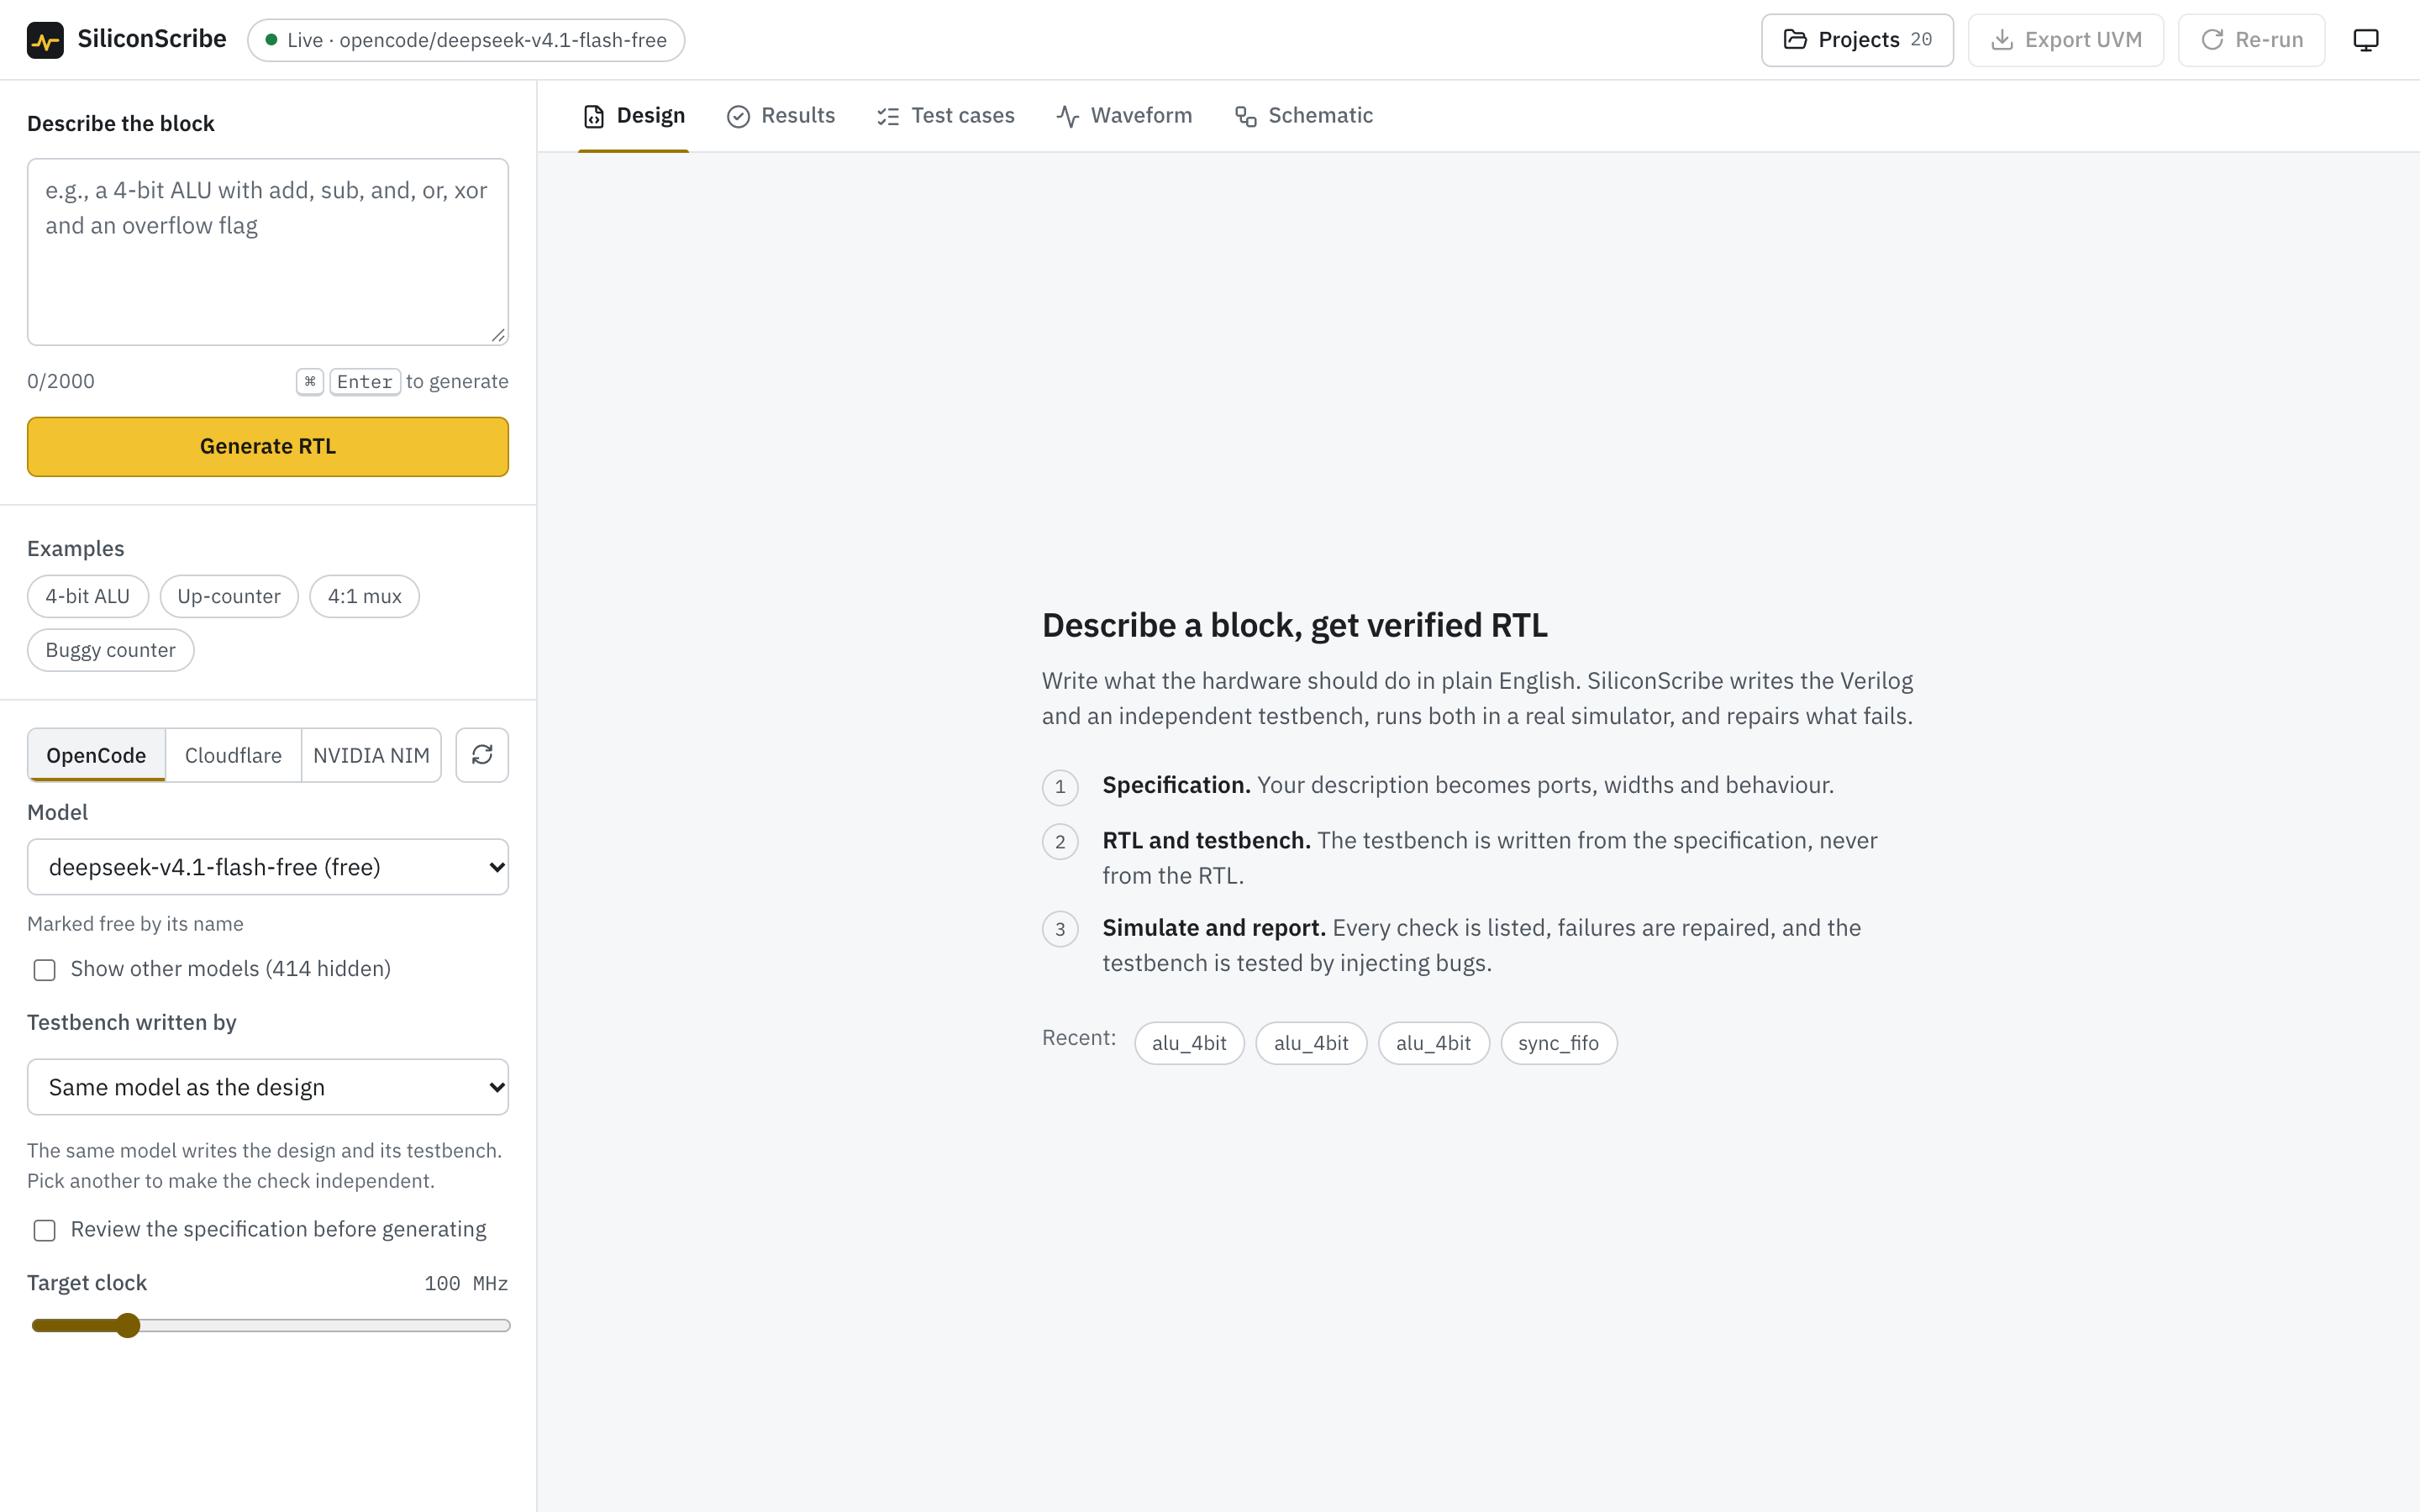
\includegraphics[width=0.85\textwidth]{figures/s01_welcome.png}
\caption{Start screen of the current build. The sidebar (left) holds the prompt box, example prompts, the per-run model menu with its OpenCode, Cloudflare and NVIDIA NIM tabs, the ``Testbench written by'' select, the ``Review the specification before generating'' checkbox and the target clock; the workspace (right) shows the Design / Results / Test cases / Waveform / Schematic tabs and a three-step explanation. The badge at the top names the live model.}
\label{fig:home}
\end{figure}

\section{Backend}
The FastAPI service exposes the endpoints of Table~\ref{tab:api}: the
full pipeline as a Server-Sent Events stream or as one JSON reply,
specification parsing, simulation, synthesis, timing, the model list, saved
projects, UVM export, and health/status endpoints. Each
design runs in an isolated workspace directory named by a 32-character design ID;
paths are validated against a strict regular expression before any file operation. Generated Verilog is additionally screened by a sandbox policy (Section~\ref{sec:sandbox}) before it is compiled.
Rate limiting is per client IP. SQLite stores project metadata and the latest
result so the history drawer can reload a design.

\section{Provider Isolation and Model Routing}
\label{sec:routing}
All model calls go through one interface in \code{llm_service.py}. Only the backend
holds credentials, and it reads them only from the git-ignored \code{backend/.env}
file, never from the web page. The default provider is chosen from the environment:
\code{OFFLINE_MODE} forces the curated offline provider; \code{LLM_PROVIDER=opencode-app}
drives the user's installed OpenCode app through its command-line interface (each
call runs in a fresh empty temporary directory with the read-only \code{plan} agent);
otherwise an OpenCode Zen, NVIDIA or OpenAI-compatible key selects that endpoint.
Per-stage overrides such as \code{LLM_MODEL_TESTBENCH} are still read from the
environment, but a model picked in the interface overrides them.

On top of this default, the user picks a model for each run from the model menu
(Figure~\ref{fig:home}), which merges three live catalogues
(Table~\ref{tab:routing}). The backend routes each request by the form of the model
identifier: \code{@cf/...} goes to Cloudflare Workers AI, \code{nim/...} goes to
NVIDIA NIM, and anything else goes to the configured provider (normally the OpenCode
app). GitHub Copilot appears only through OpenCode, as \code{github-copilot/auto}:
on the student plan GitHub picks the model and does not disclose which one, so the
result cannot name it.

\begin{table}[H]
\centering
\caption{Model sources in the per-run model menu (counts as read on 19 November 2026).}
\label{tab:routing}
\footnotesize
\begin{tabularx}{\textwidth}{@{}p{2.3cm}X p{3.3cm} p{3.7cm}@{}}
\toprule
\textbf{Source} & \textbf{How the list is obtained} & \textbf{Identifier form} & \textbf{Set up by} \\
\midrule
OpenCode app & \code{opencode models}, read live and cached; about 460 models, those whose name says free first, the rest behind ``Show other models'' & \code{opencode/<name>} & installed, signed-in OpenCode app \\
GitHub Copilot & listed by the OpenCode app & \code{github-copilot/auto} only & Copilot plan inside OpenCode \\
Cloudflare Workers AI & live catalogue through its OpenAI-compatible endpoint; 40 text models on the account & \code{@cf/<org>/<model>} & \code{CLOUDFLARE_ACCOUNT_ID}, \code{CLOUDFLARE_API_TOKEN} \\
NVIDIA NIM & live catalogue of the hosted API; 15 chat models & \code{nim/<org>/<model>} & \code{NVIDIA_NIM_API_KEY} \\
\bottomrule
\end{tabularx}
\end{table}

A model identifier comes from the browser and ends up as a subprocess argument or in a
URL, so it is checked against a strict pattern (no leading dash, no spaces or shell
characters) before it is used. A model the user chose that fails is reported in plain
words and is never replaced by the scripted demo; only the configured default keeps
the labelled offline safety net (Section~\ref{sec:fallback}). Every result records
which model wrote the design, and which wrote the testbench when they differ. The
catalogues are read live instead of being hard-coded because hosted model names
change: a NVIDIA model configured earlier in the project was retired (HTTP 410).
For a configured provider other than the OpenCode app, the menu shows the curated
list, or \emph{only} the configured model if it is not in that list. This prevents
the UI from selecting a model name the active gateway cannot serve, a real defect
found during screenshot validation (Section~\ref{sec:discussion}).

\begin{figure}[t]
\centering
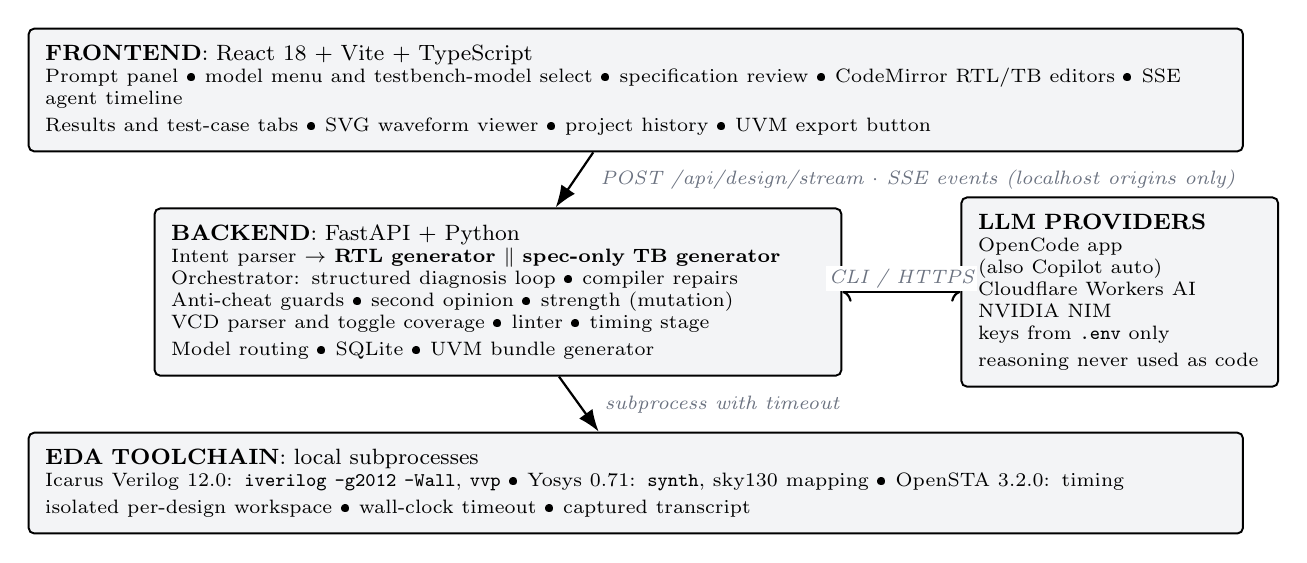
\begin{tikzpicture}[
    font=\footnotesize,
    tier/.style={draw=ink,line width=0.7pt,rounded corners=2pt,
                 fill=softgrey,align=left,
                 inner sep=6pt,minimum height=1.25cm},
    arr/.style={-{Latex[length=2.8mm]},line width=0.8pt,color=ink},
    lbl/.style={font=\scriptsize\itshape,color=rulegrey,align=center}
  ]
  \node[tier,text width=15.0cm] (fe) {\textbf{FRONTEND}: React 18 + Vite + TypeScript\\
    \scriptsize Prompt panel \textbullet\ model menu and testbench-model select \textbullet\ specification review
    \textbullet\ CodeMirror RTL/TB editors \textbullet\ SSE agent timeline\\
    \scriptsize Results and test-case tabs \textbullet\ SVG waveform viewer \textbullet\ project
    history \textbullet\ UVM export button};
  \node[tier,text width=8.3cm,below=7mm of fe,xshift=-1.75cm] (be) {\textbf{BACKEND}: FastAPI + Python\\
    \scriptsize Intent parser $\rightarrow$ \textbf{RTL generator} $\parallel$
    \textbf{spec-only TB generator}\\
    \scriptsize Orchestrator: structured diagnosis loop \textbullet\ compiler repairs\\
    \scriptsize Anti-cheat guards \textbullet\ second opinion \textbullet\ strength (mutation)\\
    \scriptsize VCD parser and toggle coverage \textbullet\ linter \textbullet\ timing stage\\
    \scriptsize Model routing \textbullet\ SQLite \textbullet\ UVM bundle generator};
  \node[tier,text width=3.6cm,right=15mm of be] (llm) {\textbf{LLM PROVIDERS}\\
    \scriptsize OpenCode app\\
    \scriptsize (also Copilot auto)\\
    \scriptsize Cloudflare Workers AI\\
    \scriptsize NVIDIA NIM\\
    \scriptsize keys from \code{.env} only\\
    \scriptsize reasoning never used as code};
  \node[tier,text width=15.0cm,below=7mm of be,xshift=1.75cm] (eda) {\textbf{EDA TOOLCHAIN}: local
    subprocesses\\
    \scriptsize Icarus Verilog 12.0: \code{iverilog -g2012 -Wall}, \code{vvp}
    \textbullet\ Yosys 0.71: \code{synth}, sky130 mapping \textbullet\ OpenSTA 3.2.0: timing\\
    \scriptsize isolated per-design workspace \textbullet\ wall-clock timeout
    \textbullet\ captured transcript};
  \draw[arr] (fe) -- node[lbl,right=2mm]{POST /api/design/stream $\cdot$ SSE events (localhost origins only)} (be);
  \draw[arr] (be) -- node[lbl,right=2mm]{subprocess with timeout} (eda);
  \draw[arr,<->] (be.east) -- node[lbl,above,fill=white,inner sep=1pt]{CLI / HTTPS} (llm.west);
\end{tikzpicture}
\caption{Three-tier architecture. RTL and testbench generation are independent
branches of the same specification; only the simulator decides PASS/FAIL.}
\label{fig:arch}
\end{figure}

\section{Data Model}
All interfaces are typed with Pydantic (Table~\ref{tab:datamodel}); invalid requests are rejected with HTTP 422 before any work starts.

\begin{table}[H]
\centering
\caption{Core data structures (\texttt{backend/models.py}).}
\label{tab:datamodel}
\footnotesize
\begin{tabularx}{\textwidth}{@{}p{3.1cm}X@{}}
\toprule
\textbf{Model} & \textbf{Key fields} \\
\midrule
\code{RTLDesignSpec} & module name, parameters, ports, behaviour, constraints \\
\code{PortSpec} & name, direction (input/output/inout), width 1--1024, description \\
\code{RunRequest} & prompt ($\le$2000 chars), frequency hint, self-correct flag, max iterations 0--10, timeout 1--120\,s, model, optional testbench model, optional confirmed specification, reasoning effort \\
\code{SimulationResult} & status, test/pass/fail counts, coverage, per-check rows and groups, measured toggle coverage, structured errors, waveform and transcript paths, log excerpt \\
\code{IterationRecord} & iteration, status, fix summary, fix type, structured diagnosis, counts, log excerpt \\
\code{RunResponse} & spec, RTL, testbench, explanation, final result, iteration history, waveform, schematic, synthesis, strength, timing, second opinion, design and testbench model, fallback notice, verification warning \\
\code{StrengthReport} & mutants run, caught, did not compile, survivors with line and description \\
\code{TimingReport} & library, clock, target and period, worst slack, met, maximum frequency, critical path, area, cell count, flip-flops, note, refusal reason \\
\code{SecondOpinion} & status (agrees / disagrees / unavailable), counts, model, note \\
\bottomrule
\end{tabularx}
\end{table}

\section{API Surface}
\begin{table}[H]
\centering
\caption{HTTP endpoints. All mutating and project routes are rate-limited to 20 requests per minute per client.}
\label{tab:api}
\footnotesize
\begin{tabularx}{\textwidth}{@{}l p{4.2cm} X@{}}
\toprule
\textbf{Method} & \textbf{Path} & \textbf{Purpose} \\
\midrule
POST & \code{/api/design/stream} & Full pipeline streamed as Server-Sent Events (used by the browser); persists the finished run \\
POST & \code{/api/design/run} & Same pipeline, single JSON response; persists the run \\
POST & \code{/api/spec/parse} & Parse a prompt into a specification and stop, for review and editing \\
POST & \code{/api/simulation/run} & Simulate a hand-edited RTL/testbench pair once \\
POST & \code{/api/synthesis/run} & Yosys synthesis if installed, otherwise an explicit unavailable result \\
POST & \code{/api/timing/run} & Pre-layout timing and mapped area on sky130 (Yosys + OpenSTA), or a reason why not \\
POST & \code{/api/uvm/export} & 16-file UVM bundle as a file map and zip \\
GET/DELETE & \code{/api/projects[/\{id\}]} & List, load or delete saved projects \\
GET & \code{/api/models} & Provider state and selectable models from the three sources; a forced refresh is rate-limited \\
POST & \code{/api/admin/cleanup} & Workspace garbage collection; disabled unless an admin token is configured \\
GET & \code{/}, \code{/health} & Status and simulator availability \\
\bottomrule
\end{tabularx}
\end{table}

\section{Event Protocol and Run Sequence}
The streaming route emits one JSON event per stage: \code{start}, \code{intent}, \code{rtl}, \code{lint}, \code{testbench}, \code{explanation}, \code{simulate}, \code{fixing}, \code{fix}, \code{synthesis}, \code{second_opinion} (only when a repair rewrote the testbench), \code{strength} and \code{timing} (only after a PASS), and finally \code{done} with the complete \code{RunResponse}, or \code{error}. Figure~\ref{fig:seq} shows the interaction for one run.

\begin{figure}[H]
\centering
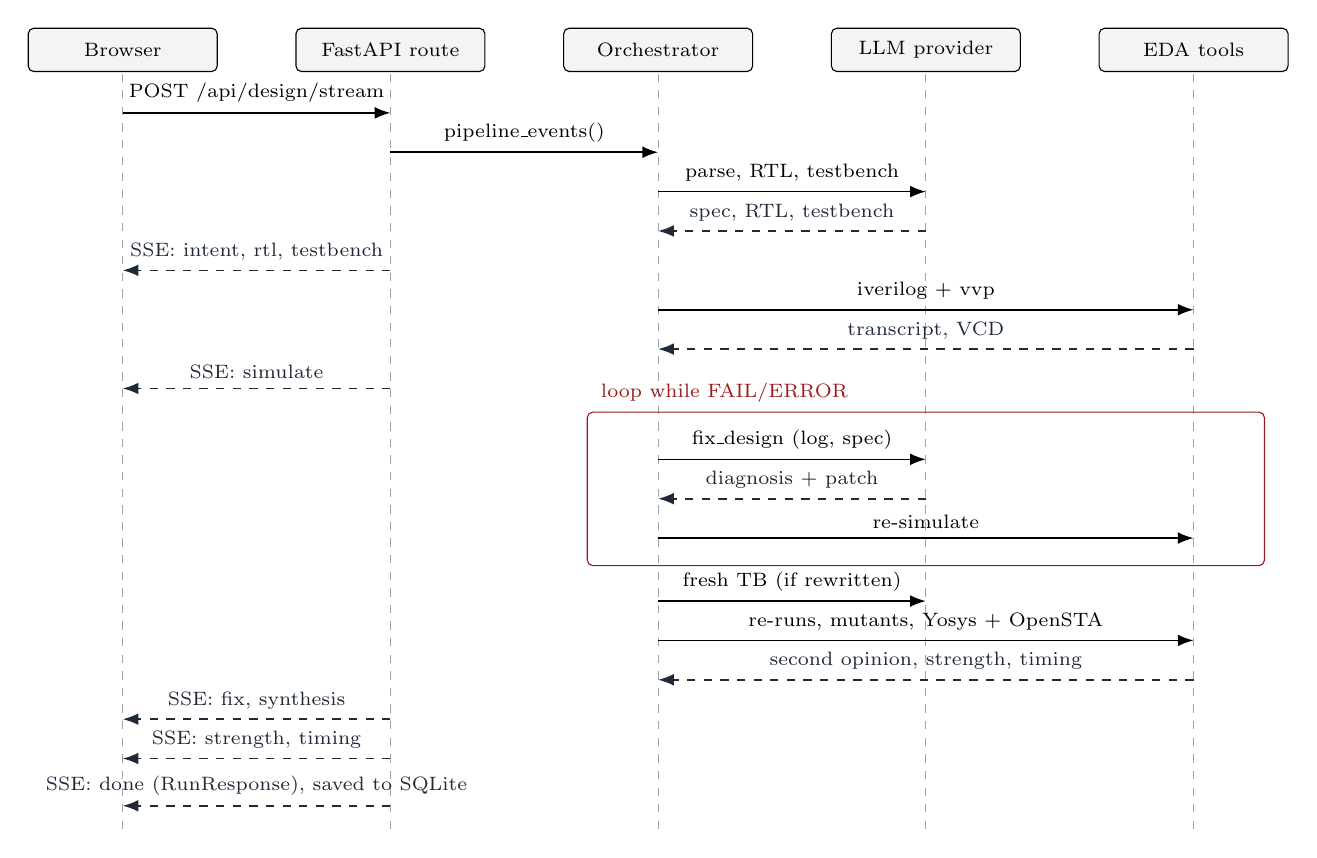
\begin{tikzpicture}[font=\scriptsize,
  actor/.style={draw=ink,fill=softgrey,rounded corners=2pt,minimum width=2.4cm,minimum height=0.55cm,align=center},
  msg/.style={-{Latex[length=2mm]},line width=0.6pt},
  ret/.style={-{Latex[length=2mm]},line width=0.6pt,dashed,color=inkdark}]
\foreach \x/\n in {0/Browser,3.4/FastAPI route,6.8/Orchestrator,10.2/LLM provider,13.6/EDA tools}{
  \node[actor] at (\x,0) {\n};
  \draw[dashed,color=midgrey] (\x,-0.3) -- (\x,-9.9);}
\draw[msg] (0,-0.8) -- node[above]{POST /api/design/stream} (3.4,-0.8);
\draw[msg] (3.4,-1.3) -- node[above]{pipeline\_events()} (6.8,-1.3);
\draw[msg] (6.8,-1.8) -- node[above]{parse, RTL, testbench} (10.2,-1.8);
\draw[ret] (10.2,-2.3) -- node[above]{spec, RTL, testbench} (6.8,-2.3);
\draw[ret] (3.4,-2.8) -- node[above]{SSE: intent, rtl, testbench} (0,-2.8);
\draw[msg] (6.8,-3.3) -- node[above]{iverilog + vvp} (13.6,-3.3);
\draw[ret] (13.6,-3.8) -- node[above]{transcript, VCD} (6.8,-3.8);
\draw[ret] (3.4,-4.3) -- node[above]{SSE: simulate} (0,-4.3);
\draw[draw=failred,rounded corners=2pt] (5.9,-4.6) rectangle (14.5,-6.55);
\node[anchor=south west,color=failred] at (5.95,-4.6) {loop while FAIL/ERROR};
\draw[msg] (6.8,-5.2) -- node[above]{fix\_design (log, spec)} (10.2,-5.2);
\draw[ret] (10.2,-5.7) -- node[above]{diagnosis + patch} (6.8,-5.7);
\draw[msg] (6.8,-6.2) -- node[above]{re-simulate} (13.6,-6.2);
\draw[msg] (6.8,-7.0) -- node[above]{fresh TB (if rewritten)} (10.2,-7.0);
\draw[msg] (6.8,-7.5) -- node[above]{re-runs, mutants, Yosys + OpenSTA} (13.6,-7.5);
\draw[ret] (13.6,-8.0) -- node[above]{second opinion, strength, timing} (6.8,-8.0);
\draw[ret] (3.4,-8.5) -- node[above]{SSE: fix, synthesis} (0,-8.5);
\draw[ret] (3.4,-9.0) -- node[above]{SSE: strength, timing} (0,-9.0);
\draw[ret] (3.4,-9.6) -- node[above]{SSE: done (RunResponse), saved to SQLite} (0,-9.6);
\end{tikzpicture}
\caption{Sequence of one streamed run. Guards inside the loop can stop it early (Figure~\ref{fig:loop}). The checks after the loop run only after a PASS; the fresh testbench is requested only when a repair rewrote the testbench.}
\label{fig:seq}
\end{figure}

\section{Timing and Area Stage}
\label{sec:timingarch}
After a PASS, and only when Yosys, OpenSTA and the cell library are installed,
\code{timing.py} gives an early estimate of whether the logic is near the target
clock. When a tool is missing the result simply has no timing section; nothing is
estimated. The flow has two steps:

\begin{enumerate}[label=\textbf{\arabic*.}]
\item \textbf{Mapping.} Yosys 0.71 (the yowasp WebAssembly build) flattens the
hierarchy and maps the design to \code{sky130_fd_sc_hd} standard cells at the
typical corner (25\,\textdegree C, 1.8\,V). Parameters that the testbench overrides
are applied first, so the circuit timed is the circuit simulated.
\item \textbf{Timing.} OpenSTA 3.2.0 (built from source) reads the mapped netlist and
the liberty file. Clocks are read from the netlist (the nets the flip-flops are
really wired to), so any port name and several clocks are handled.
\end{enumerate}

For a clocked design the report gives the worst setup slack at the target clock and
the minimum clock period (maximum frequency). A design with no clock is reported by
its longest input-to-output path, never as a clock rate. Every report also gives the
critical path, the mapped area in \textmu m$^2$, the cell count and the number of
flip-flops. The limits are stated in the app: one typical corner, no placement or
routing (so no wire delay), an ideal clock, zero input/output delays and setup
analysis only. It is not sign-off, and power is not reported. Instead of printing
a number it cannot justify, the stage refuses with a reason for tri-states (Yosys
would silently turn them into wires), latches, combinational loops, derived or gated
clocks and designs with no logic cells. The same stage is available on its own
through \code{/api/timing/run}. How its numbers were checked is described in
Section~\ref{sec:gatelevel}.

\section{Second-Opinion and Independent-Testbench Flow}
\label{sec:secondarch}
Both paths below give a second reading of the specification, because a testbench
written by the same model as the design can share its misreading.

\textbf{Independent testbench.} When \code{testbench_model} names a different model
(it may be from another provider), the testbench stage, and any second opinion, is
routed to that model. In the repair loop the design model may still change the RTL,
but it may not rewrite a testbench that compiled and ran: a failing check is
reported, never rewritten away. Only a testbench that does not compile or hangs may
be repaired. If the run ends in FAIL, the result names both models and says that
either the design or the testbench misreads the specification; the tool does not
decide automatically which side is wrong.

\textbf{Second opinion.} A PASS that came only after a repair rewrote the testbench is
the weakest kind of PASS. Two extra checks then run on the final design. First, the
\emph{original} testbench is re-run; if it still fails, a warning is attached.
Second, a fresh testbench is generated from the same specification, validated (it
must instantiate the design and contain checks) and simulated. The outcome is shown
as ``agrees'' (PASS), ``disagrees'' (FAIL, which puts a warning on the PASS) or
``unavailable'' (the fresh testbench could not be generated or did not run cleanly).
A failure inside these extra checks never breaks a run that has already been verified.

\section{Persistence Schema}
Projects are stored in one SQLite table with columns \code{id}, \code{prompt}, \code{module_name}, \code{rtl_spec}, \code{rtl_code}, \code{testbench_code}, \code{explanation}, \code{status}, \code{pass_count}, \code{fail_count}, \code{iterations}, \code{created_at}, \code{waveform_truncated} and a JSON \code{data} column holding the full response. Every call opens its own connection, so the thread-pooled routes do not share connection state.

\section{Security Design}
\label{sec:security}
\begin{itemize}
\item \textbf{Input limits:} prompt 2000 characters, RTL/testbench 50\,000 characters, 200\,KB per written file, timeouts 1--120\,s, iterations 0--10, identifiers validated by regular expression.
\item \textbf{Path safety:} design IDs match \code{^[a-zA-Z0-9_-]\{1,32\}$}; every path is resolved and checked to stay inside the workspace, including through symbolic links.
\item \textbf{Execution:} compile timeout 30\,s, simulation timeout, sandbox policy (system tasks on an allow-list), scrubbed environment, CPU, file-size and memory limits (the memory limit is enforced on Linux only), and at most two simulations at once (Section~\ref{sec:sandbox}).
\item \textbf{Abuse control:} per-IP sliding-window rate limit (by the socket peer unless proxy headers are trusted on purpose); admin cleanup requires a token compared in constant time.
\item \textbf{Model identifiers:} validated against a strict pattern before they reach a subprocess or a URL (Section~\ref{sec:routing}).
\item \textbf{Information hygiene:} internal errors return a generic message; API keys are read only from \code{backend/.env}, stay server-side and are never written to git, the frontend bundle or the logs (checked by a scan); the API accepts browser calls from this machine only (CORS limited to localhost origins), and further exact origins must be added on purpose through \code{CORS_ALLOW_ORIGINS}, with no wildcard.
\end{itemize}

    \chapter{Methodology}
\label{sec:method}

\section{Specification Parsing}
The first live call converts the prompt into an \code{RTLDesignSpec}: module name,
parameters, ports (name, direction, width, description), behavioural rules, and
constraints. The parser prompt requires the specification to pin down every
observable behaviour, including reset polarity, opcode tables, priority order, and
the value of all outputs for all input combinations. This is essential because the
RTL and testbench generators never see each other's output.

\subsection{Specification Review}
\label{sec:specreview}
The specification is itself written by a model, so it can misread the prompt, and a
testbench derived from a wrong specification would agree with a wrong design. The
optional ``Review the specification before generating'' setting therefore stops after
parsing (\code{/api/spec/parse}) and shows the module name, ports, behaviour and
constraints (Figure~\ref{fig:specreview}). The user can edit the behaviour and the
constraints, and the run then uses exactly that specification: the parsing step is
skipped. A user specification is treated as untrusted input: its names end up in file
names, patterns and prompts, so they must be plain identifiers, and its text is
bounded in size. The specification that was used is
shown read-only with the results.


\section{Independent, Specification-Derived Testbenches}
\label{sec:tb}
The testbench generator receives only the parsed specification; the RTL body is
withheld. This breaks the circular verification of the earlier progress report, in
which the same model could write a DUT and a testbench that were consistently wrong
together. The prompt requires:

\begin{itemize}
\item a top module named \code{testbench}, with explicit named port connections;
\item clock/reset generation for sequential DUTs;
\item directed corner cases \emph{and} at least 100 randomized vectors;
\item expected values computed from the specification, compared with \code{===};
\item integer \code{pass_count}/\code{fail_count} and exact summary lines;
\item \code{\$dumpfile}/\code{\$dumpvars} for the waveform;
\item Verilog-2001/Icarus compatibility: module-scope declarations only, no
\code{break}, \code{continue}, or \code{disable} of a function; a first-match
\code{if/else-if} chain or a \code{found} flag for priority logic; width-correct
comparisons.
\end{itemize}

These rules were not written speculatively. Each one corresponds to a real failure
observed in a live run (Section~\ref{sec:discussion}). The testbench also prints one
machine-readable \code{CHK|...} line per comparison (result, category, name, time,
expected and actual value), which the Test cases tab lists. If the user chose a
separate testbench model, this stage runs on that model (Section~\ref{sec:secondarch}).

\section{Execution}
The orchestrator writes \code{design.sv} and \code{testbench.sv} into the workspace,
compiles with \code{iverilog -g2012 -Wall -o testbench.vvp}, and runs
\code{vvp} under a configurable wall-clock timeout. Compilation diagnostics are
parsed into structured errors. PASS/FAIL is decided by this execution, never by
model text, using the rules below.

\section{Verdict Integrity}
\label{sec:verdict}
The testbench prints its own summary, so the parser must not trust the first or the
loosest match. Earlier versions did, and a review reproduced three problems: a
mid-run phase line could decide the verdict, an uninitialised \code{Failed: x} was
read as zero, and \code{ALL TESTS PASSED} overrode printed errors. The rules are now:

\begin{itemize}
\item the \code{Passed:} and \code{Failed:} summary lines must each occupy a whole
line, the last pair wins, and both counts must be numbers, otherwise the run is
ERROR;
\item any \code{FAIL}, \code{ERROR} or \code{FATAL} line contradicts \code{Failed: 0}
and makes the run FAIL;
\item at least one check must have executed: \code{Passed: 0} is ERROR, never PASS;
\item a simulator exit code other than zero (for example killed by a resource limit)
is ERROR;
\item the design under test may not print the summary lines or end the simulation
(\code{$finish}, \code{$stop}, \code{$fatal} are refused in the RTL), so it cannot
write its own verdict;
\item a testbench whose watchdog stops the run before the summary is printed has no
valid summary, so the run is ERROR.
\end{itemize}

The \code{CHK|...} rows are display data: they are size-capped and cross-checked
against the summary, but they never decide the verdict. The watchdog rule was seen
live: a Cloudflare model wrote a correct counter but a testbench whose watchdog was
shorter than its own test, and the run was reported as ERROR with zero checks
instead of PASS. A PASS is still evidence, not proof, which is why the measurements
in Section~\ref{sec:evidence} exist.

\section{Execution Sandbox Policy}
\label{sec:sandbox}
Generated or user-edited Verilog is executed by \code{vvp} with the server's privileges, so it is untrusted input. The final-review probe (Section~\ref{sec:review}) showed that Verilog file-I/O system tasks (\code{$fopen}, \code{$fgets}, \code{$fwrite}, \code{$readmemh} and related tasks) could read or write any path the process could reach, and that the contents came back in the API response. Three independent controls now apply to every simulation, and the static policy also runs before lint, synthesis and timing:

\begin{enumerate}[label=\textbf{\arabic*.}]
\item \textbf{Static policy.} Before anything is compiled, the RTL and testbench are scanned. System tasks are an allow-list: anything not on it, including \code{$system}, file I/O and \code{$readmemh}, is refused, as are the include directive, macro token pasting, and a \code{$dumpfile} argument that is not a plain file name. The scan deliberately does not strip comments: a naive comment stripper can be fooled by a double slash inside a string literal into hiding a forbidden call.
\item \textbf{Scrubbed environment.} The compiler and simulator run with a minimal environment (path, locale and temporary directory only), so API keys held by the server never reach them.
\item \textbf{Resource limits.} The simulator runs under file-size, CPU-time and memory limits (the memory limit is enforced on Linux, not on macOS), so a runaway \code{$display} loop cannot fill the disk before the wall-clock timeout; at most two simulations run at once.
\end{enumerate}

This is defence in depth, not a security boundary: a static scan of a language as flexible as Verilog can never be airtight. For multi-user deployment the simulator must run inside a container or jail (Section~\ref{sec:scale}).

\section{Structured Diagnosis and Repair}
\label{sec:loop}
When the result is FAIL or ERROR, the fixer receives the RTL, the testbench, the
specification, and the simulator log. It must answer in explicit sections:

\begin{lstlisting}[language=,basicstyle=\ttfamily\scriptsize]
<diagnosis>
symptom: <what the log shows, with the first failing vector>
root_cause: <the hardware reason, not a restatement of the symptom>
fix_location: <file / module / line / signal>
confidence: high|medium|low
</diagnosis>
<rtl> ... complete corrected RTL ... </rtl>
<testbench> ... complete testbench ... </testbench>
<summary> ... one sentence ... </summary>
\end{lstlisting}

The section format replaced a fragile JSON response after a live run produced
malformed JSON with unescaped Verilog newlines and quotes. A tolerant JSON path and
a field-salvage path remain for older models, but compliant models use the section
format.

The fixer is explicitly instructed to check the \emph{testbench oracle} against the
specification: if the RTL matches the spec but the expected-value logic does not,
the bug is in the testbench. This is a real failure mode: one generated testbench
concatenated a 32-bit integer with a 3-bit code, making a 35-bit comparison that
could never equal the 4-bit DUT output.

Figure~\ref{fig:loop} shows the control flow. A patch is rejected if it removes
self-checks from a testbench that already compiled and ran. The loop also tracks a
comment/whitespace-normalised hash of \emph{both} RTL and testbench; an unchanged
state is a no-op, and a repeated state is oscillation. Both terminate the loop
instead of burning tokens. The loop runs for at most five iterations by default.
When a separate model wrote the testbench, the design model may not change a
testbench that compiled and ran at all; it may only repair one that does not compile
or hangs. After a repair that changed the testbench, the original testbench is
re-run on the final design and a second-opinion testbench is requested
(Section~\ref{sec:secondarch}).


\section{Deterministic Compiler Repairs}
Some failures are not design decisions and should not be delegated to a model:

\begin{itemize}
\item \textbf{wire$\rightarrow$reg.} Icarus reports
\code{X is not a valid l-value} when a net is assigned from a procedural block. The
repair is scoped to the file named in the diagnostic, changes only that declaration,
and is recorded as \code{fix_type="compiler_repair"} with a real diagnosis.
\item \textbf{disable$\rightarrow$return.} Icarus rejects \code{disable <function>}
inside a function but accepts \code{return <function>}. The repair preserves the
first-match semantics of the oracle.
\end{itemize}

Neither repair touches the testbench's checks; both are labelled as compiler
repairs in the UI and in \code{iteration_history}.

\section{Honest Degraded Mode}
\label{sec:fallback}
The offline curated designs remain available for demonstrations and for the
automated suite, but the policy is explicit:

\begin{itemize}
\item If the provider is unreachable \emph{before any live artifact exists}, the
pipeline may fall back to a curated design and attaches a visible
\code{fallback_notice}. The UI shows a degraded-mode banner.
\item Once a live call has succeeded, a later outage raises an error. The run does
not silently swap the user's design mid-flight.
\item Scripted offline fixes return \code{diagnosis=None} and
\code{fix_type="offline_scripted"}. They never fabricate a root cause.
\item The offline fallback applies only to the configured default model. A model the
user picked on purpose (or a separate testbench model) that fails is reported in
plain words and the user picks another; it is never replaced by the demo.
\end{itemize}

For demonstrations the fallback ladder is therefore: the live model, then the
labelled offline scripted demo, then saved results of earlier live runs.

This policy was added after an early live run silently switched to a curated design
when the provider failed, producing a PASS that did not correspond to the prompt.

\begin{figure}[H]
\centering
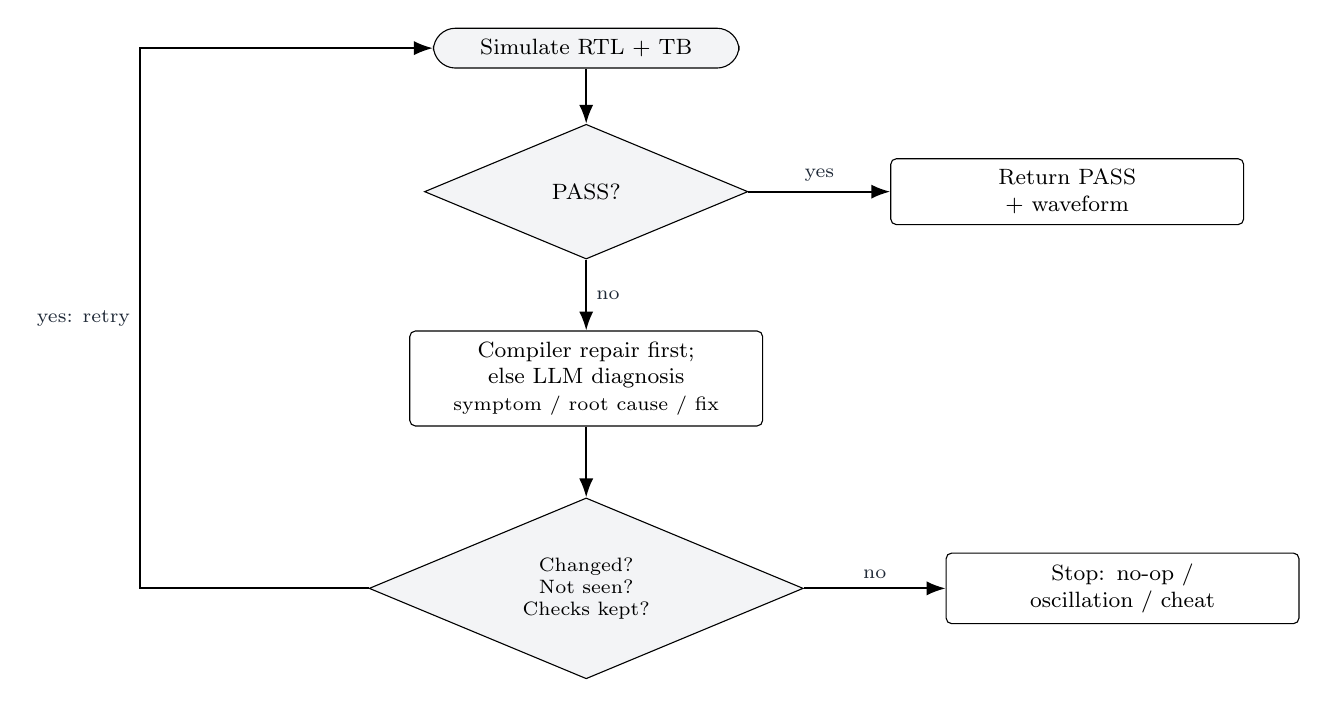
\begin{tikzpicture}[
    font=\footnotesize,
    start/.style={draw=ink,rounded corners=8pt,fill=softgrey,text width=3.6cm,align=center,inner sep=4pt},
    proc/.style={draw=ink,rounded corners=2pt,fill=white,text width=4.2cm,align=center,inner sep=4pt},
    dec/.style={draw=ink,diamond,aspect=2.4,fill=softgrey,text width=3.4cm,align=center,inner sep=1pt},
    arr/.style={-{Latex[length=2.4mm]},line width=0.7pt},
    lbl/.style={font=\scriptsize,color=inkdark}
  ]
  \node[start] (sim) {Simulate RTL + TB};
  \node[dec,below=7mm of sim] (ok) {PASS?};
  \node[proc,below=9mm of ok] (diag) {Compiler repair first;\\else LLM diagnosis\\
    \scriptsize symptom / root cause / fix};
  \node[dec,below=9mm of diag,font=\scriptsize] (guard) {Changed?\\Not seen?\\Checks kept?};
  \node[proc,right=18mm of ok] (done) {Return PASS\\+ waveform};
  \node[proc,right=18mm of guard] (stop) {Stop: no-op /\\oscillation / cheat};
  \draw[arr] (sim) -- (ok);
  \draw[arr] (ok) -- node[lbl,above]{yes} (done);
  \draw[arr] (ok) -- node[lbl,right]{no} (diag);
  \draw[arr] (diag) -- (guard);
  \draw[arr] (guard) -- node[lbl,above]{no} (stop);
  \draw[arr] (guard.west) -- ++(-2.9,0) |- node[lbl,left,pos=0.25]{yes: retry} (sim.west);
\end{tikzpicture}
\caption{Diagnosis and repair loop. Mechanical compiler repairs run before the LLM;
the simulator is the only oracle. A patch that removes testbench checks, changes
nothing, or repeats a previous state terminates the loop.}
\label{fig:loop}
\end{figure}


\section{Orchestration Algorithm}
\begin{lstlisting}[language=,basicstyle=\ttfamily\scriptsize,caption={Self-correction loop as implemented in orchestrator.py (simplified).},label={lst:algo}]
spec   = parse_intent(prompt)            # offline fallback only before any live call
rtl    = generate_rtl(spec)              # must contain a complete module; one retry
tb     = generate_testbench(spec)        # RTL withheld; must instantiate DUT and self-check
result = simulate(rtl, tb); seen = {hash(rtl, tb)}
for i in 1..max_iterations while result in {FAIL, ERROR}:   # default 5
    if result == ERROR and compiler_repair applies:      # wire->reg, disable->return
        apply repair; result = simulate(rtl, tb); continue
    fix = fix_design(rtl, tb, log, spec)                  # diagnosis + full patched files
    if result != ERROR and checks(fix.tb) < checks(tb):   # anti-cheat
        fix.tb = tb
    if separate_tb_model and result != ERROR:             # a failing check is reported,
        fix.tb = tb                                       # never rewritten away
    h = hash(fix.rtl, fix.tb)                             # whitespace/comment-insensitive
    if h == hash(rtl, tb): stop("no-op")
    if h in seen:          stop("oscillation")
    seen.add(h); rtl, tb = fix.rtl, fix.tb; result = simulate(rtl, tb)
if PASS and tb != original_tb:                            # testbench was rewritten
    rerun(original_tb); second = simulate(rtl, generate_testbench(spec))
if PASS: strength = mutants(rtl, tb); timing = yosys_opensta(rtl)  # + equivalence proof
return result, history, waveform, schematic, synthesis, strength, timing, second
\end{lstlisting}

\section{Measuring the Evidence behind a PASS}
\label{sec:evidence}
A PASS only says that the testbench found nothing wrong. The checks in this section
ask how much that is worth. None of them can change a verdict; they add
information and warnings to it.

\subsection{Testbench Strength by Mutation}
\label{sec:strength}
After a PASS, \code{mutation.py} applies mutation testing~\cite{demillo} to the
design: it makes up to 12 one-token changes (\code{+} to \code{-}, \code{&} to
\code{|}, \code{==} to \code{!=}, a flipped constant or case label, a negated
\code{if}, and similar) and runs the \emph{same} testbench against each changed copy.
Comments, strings, directives, parameters, bit ranges and loop headers are not mutated. The score
is bugs caught divided by bugs run; a mutant that does not compile is not counted.
The whole check has a time budget of 40\,s and each mutant 6\,s, so a hanging mutant
cannot block the run. When at least five mutants ran and fewer than half were caught,
the PASS is flagged as weak evidence. A surviving mutant may be \emph{equivalent}
(the changed design behaves identically), so a survivor means ``not detected'', not
``proven missed''.

\subsection{Measured Toggle Coverage}
Toggle coverage is read from the simulator's own VCD file. A bit counts as covered
only when it is seen going directly from 0 to 1 and from 1 to 0 (a change through
\code{x} or \code{z} does not count), and only nets inside the instantiated design
are counted, so testbench bookkeeping cannot raise the number. Signals that never
toggled are listed bit by bit. Line and branch coverage are \emph{not} measured.
Verilator~\cite{verilator} was tried for them and rejected: only 3 of 12 designs built
with its pip-installed release, and the testbenches of two evaluated designs (c3, c4)
hit an ``unsupported tristate construct'' error. Any other coverage number that a
testbench prints about itself is shown as self-reported.

\subsection{Gate-Level Check of the Mapped Netlist}
\label{sec:gatelevel}
The timing and area numbers of Section~\ref{sec:timingarch} are only useful if the
mapped netlist is the same circuit as the RTL. The script
\code{tools/verify_mapping.py} checks this three ways, none of which reads the number
it checks from the same place:

\begin{enumerate}[label=\textbf{\arabic*.}]
\item \textbf{Gate-level simulation.} Yosys writes behavioural models of the sky130
cells from the liberty file; the mapped netlist is simulated in Icarus with the
\emph{same} testbench as the RTL and must give identical pass and fail counts.
\item \textbf{Area recount.} Area and cell count are recomputed from the written
netlist and the liberty file and must equal what Yosys reported.
\item \textbf{Timing sanity.} The design is timed at a second target clock; the
implied minimum period (period minus slack) must not change.
\end{enumerate}

A design that the stage refuses on purpose (latch, tri-state, derived clock) is
reported as such and is not a failure. The checker was itself tested on sabotaged
netlists, which it caught. On the final code all 19 checked designs (the built-in
designs and the saved evaluation designs) gave the same results at gate level. This is a
simulation-based check with the project's testbenches, so it is only as complete as
those testbenches. The formal check below does not depend on a testbench.

\subsection{Formal Equivalence of the Mapped Netlist}
\label{sec:equiv}
After mapping, \code{equivalence.py} tries to prove that the sky130 netlist and the
RTL are the same circuit. It uses only Yosys' built-in SAT (Boolean satisfiability)
solver, so no external solver is installed. The netlist cells are read from the
liberty file's own logic functions, so the proof is about the real cells and not
about a hand-written model of them, and the RTL gets the same testbench parameter
overrides that were used for the mapping.

\begin{itemize}
\item \textbf{Combinational designs.} The RTL (``gold'') and the netlist (``gate'')
are placed side by side in a \emph{miter}: both get the same inputs and their outputs
are compared. The SAT solver is then asked for any input value that makes an output
differ. If none exists the design is proven equivalent over every defined input
value. Inputs are restricted to 0 and 1, because \code{x} is not a real hardware
input; with \code{x} allowed, SAT reported a false mismatch on a correct ALU
(Table~\ref{tab:review3}). If SAT finds such a value, the result is ``different''.
\item \textbf{Sequential designs.} The registers of the two designs are paired by
name (\code{equiv_make}) and each pair is proven equal by temporal
induction~\cite{sheeran} (\code{equiv_simple} and \code{equiv_induct}): if all
pairs are equal in one cycle, they stay equal in the next. The design is proven only
when every register and output point is proven.
\item \textbf{Undecided cases.} When synthesis re-encodes the state of an FSM, the
registers no longer pair up by name and induction cannot decide. The result is then
``not proven'', never a pass and never a failure. The gate-level simulation check
of Section~\ref{sec:gatelevel} still applies.
\end{itemize}

What the proof shows is narrow: the netlist that the timing and area numbers describe
computes the same function as the RTL that was simulated. It says nothing about
whether the RTL itself does what the prompt asked; that question is answered only by
the testbench, the strength score and the independent reference testbenches.

\subsection{Critical Path Report}
\label{sec:critpath}
The timing section also lists the worst path from OpenSTA's \code{report_checks}
output pin by pin: the pin, the sky130 cell, rise or fall, the incremental delay and
the arrival time (\code{critical_path_rows} in \code{timing.py}). Only the data path
up to the data arrival time is kept, so clock-tree pins are not mixed into it. The
table shows where the time goes, for example a ripple-carry chain
(Section~\ref{sec:equivres}).

\subsection{Independent Reference Testbenches}
\label{sec:reftb}
Strength measures the model's testbench, not the design. To check the designs
themselves, a reference testbench was written by hand (not by a model) for every
evaluated design (kept in \texttt{evaluation/\allowbreak independent/}). Each one compares the design with
a reference model and reports a mismatch count; a design is CORRECT only with zero
mismatches. The references were measured in turn: every one-token mutant that the
app's generator can make (not just a sample of 12) was run against them, and each
survivor was reviewed by hand.

\section{Evaluation Protocol}
\label{sec:evalprotocol}
The live evaluation uses a fixed set of 15 prompts (Table~\ref{tab:evalprompts}),
easy to moderate, spread over 7 combinational, 6 sequential and 2 FSM designs. Each
prompt was run once through the real pipeline by \code{tools/evaluate_live.py}, with
the free DeepSeek V4.1 Flash model through the OpenCode app writing both the design
and the testbench. The rules were fixed before the runs:

\begin{itemize}
\item one JSON record per finished prompt is written immediately, and a re-run
resumes, so a free-tier cut-off loses nothing;
\item a provider outage or quota error stops the run and is not recorded as a design
failure;
\item a run that fell back to the offline demo is recorded as a fallback and is not
counted;
\item a prompt that never completes is reported as ``no result'', never as a pass or
a failure;
\item for each completed prompt the record keeps the verdict, the number of repairs,
the check counts, the strength score, the measured toggle coverage, the timing and
area estimate and the run time;
\item every passing design is then checked against its independent reference
testbench (Section~\ref{sec:reftb}), which answers whether a PASS was a false PASS.
\end{itemize}

The evaluation calls the pipeline directly, so it does not write to the projects
database. The results are reported in Section~\ref{sec:eval}.


    \chapter{Implementation and Testing}
\label{sec:impl}

\begin{table}[H]
\centering
\caption{Principal implementation modules (all paths under \texttt{backend/} or
\texttt{frontend/src/}).}
\label{tab:modules}
\footnotesize
\begin{tabularx}{\textwidth}{@{}p{4.0cm}p{6.6cm}X@{}}
\toprule
\textbf{Module} & \textbf{Responsibility} & \textbf{Key idea} \\
\midrule
\code{main.py} & FastAPI routes, SSE streaming, rate limiting, CORS & one event stream per design \\
\code{orchestrator.py} & pipeline, repair loop, guards, fallback policy, second opinion & simulator decides; anti-cheat \\
\code{llm_service.py} & provider config, prompts, fix parser, per-stage model routing & spec-only TB; section protocol \\
\code{model_catalog.py} & model menu: OpenCode, Cloudflare Workers AI, NVIDIA NIM & catalogues read live; ids validated \\
\code{simulator.py} & workspace, iverilog/vvp, log parsing, sandbox policy & isolated, timed, policy-screened execution \\
\code{vcd_parser.py} & VCD $\rightarrow$ JSON waveform; toggle coverage & bounded size; design signals only \\
\code{mutation.py} & testbench strength by mutation testing & up to 12 one-token bugs per PASS \\
\code{timing.py} & Yosys mapping to sky130 cells, OpenSTA timing, area, critical path & pre-layout estimate; refuses what it cannot time \\
\code{equivalence.py} & formal equivalence of the mapped netlist and the RTL & Yosys SAT; ``not proven'' is never a pass \\
\code{linter.py} & Verilator $\rightarrow$ Icarus $\rightarrow$ regex & graceful degradation \\
\code{synthesis.py}, \code{schematic.py} & Yosys wrapper (generic cell counts), netlists for the schematic views & optional; honest unavailable state \\
\code{db.py} & SQLite persistence, project retrieval & zero-dependency storage \\
\code{uvm_templates.py} & 16-file UVM 1.2 bundle & export-only, CI file-count check \\
\code{tools/} & mutation sweep, mapping check, preflight, live evaluation & reproducible evidence \\
\code{App.tsx} & SSE client, project state, export & live timeline, fallback banner \\
\code{ModelPicker.tsx} and others & model menu, ``Testbench written by'', specification review & per-run choice, remembered \\
\code{ResultsPanel.tsx} & PASS/FAIL, metrics, strength, coverage, timing, second opinion, tabs & iteration history, expand to full window \\
\code{TestCasesView.tsx} & per-test-case table & test types, filters, bit-level diff, jump to waveform \\
\code{WaveformViewer.tsx} & SVG waveform & role groups, value at cursor, two cursors, radix, failed-check flags \\
\code{SchematicView.tsx} & block, RTL-cell and gate-level schematic & netlistsvg in the browser; at most 400 cells drawn \\
\bottomrule
\end{tabularx}
\end{table}

The backend is Python 3.14 with FastAPI, Pydantic, and the OpenAI Python client
pointed at an OpenAI-compatible base URL; the OpenCode app is driven through its
command-line interface. The frontend is React 18, TypeScript, Vite, and CodeMirror.
Icarus Verilog 12.0 is the simulator. Yosys~\cite{yosys} and OpenSTA~\cite{opensta}
are used for the timing and area estimate; if either tool or the cell library is
missing, the API reports the estimate as not available instead of inventing numbers.

\section{Test Strategy}
The backend suite has 589 tests in 35 files: data models and validation, linter behaviour,
simulator and VCD parsing, toggle coverage, API edge cases, orchestrator
repair/fallback/guard paths, LLM response parsing (XML sections, malformed JSON
salvage, literal newlines), verdict integrity, the sandbox policy, mutation testing,
the timing and area stage, the formal equivalence check and the critical path, the model catalogue and model switching, the separate
testbench model, the specification review and the verification tools themselves. The
suite runs against a throw-away workspace and never touches the developer's
database. The frontend suite has 259 Vitest tests in 18 files, including an automated
accessibility audit with axe-core. The mutation tests are the important ones: they take a
curated design, inject a semantic bug (wrong increment, missing reset, wrong mux
select, wrong ALU opcode), and assert that the testbench reports FAIL. A testbench
that cannot fail is not evidence. The newest components were also checked the other
way round: each behaviour was broken on purpose and the tests had to fail. Beyond
the unit and integration tests, scripts check the tool's own measurements
(Section~\ref{sec:trustimpl}), and live runs against real models validate the whole
pipeline (Chapter~\ref{sec:results}).

\section{Technology Stack}
\begin{table}[H]
\centering
\caption{Technology stack on the validation machine (Apple M4, macOS).}
\label{tab:stack}
\footnotesize
\begin{tabularx}{\textwidth}{@{}p{2.4cm}X@{}}
\toprule
\textbf{Layer} & \textbf{Components} \\
\midrule
Backend & Python 3.14.2, FastAPI, Uvicorn, Pydantic 2, OpenAI Python client (pinned in \code{requirements.txt}; the machine ran FastAPI 0.141.1, Pydantic 2.13.5) \\
Frontend & React 18.3, TypeScript 5.7, Vite 6, CodeMirror 6, Vitest 4 with Testing Library, jsdom and axe-core \\
EDA & Icarus Verilog 12.0~\cite{icarus}; Yosys 0.71 (YoWASP WebAssembly build); OpenSTA 3.2.0 built from source; SkyWater SKY130 \code{sky130_fd_sc_hd} typical-corner liberty~\cite{sky130}; Verilator optional for lint (not installed on this machine) \\
Model sources & OpenCode app (v2.3.2 on this machine), Cloudflare Workers AI, NVIDIA NIM; any other OpenAI-compatible endpoint through environment variables \\
Operations & Docker multi-stage image, Docker Compose, GitHub Actions CI, Vercel (frontend) and Render (backend) free tiers \\
\bottomrule
\end{tabularx}
\end{table}

\section{Implementation of the Measurement and Trust Stages}
\label{sec:trustimpl}
The design of the newer stages is described in Chapters~\ref{sec:arch}
and~\ref{sec:method}: model routing (Section~\ref{sec:routing}), timing and area
(Section~\ref{sec:timingarch}) with its equivalence proof (Section~\ref{sec:equiv}), the separate testbench model and the second opinion
(Section~\ref{sec:secondarch}), and the evidence measures (Section~\ref{sec:evidence}).
Table~\ref{tab:trustimpl} records where each one lives in the code and the
implementation details that matter. Every stage after the verdict follows the same
rule: a failure inside it never breaks a verified run; it reports ``not available''
with a reason instead.

\begin{table}[H]
\centering
\caption{Where the newer stages are implemented, and the details that matter.}
\label{tab:trustimpl}
\footnotesize
\begin{tabularx}{\textwidth}{@{}p{2.5cm}p{2.9cm}X@{}}
\toprule
\textbf{Stage} & \textbf{Code} & \textbf{Implementation details} \\
\midrule
Testbench strength & \code{mutation.py} & up to 12 one-token mutants (\code{STRENGTH_MAX_MUTANTS}), each run in the same sandboxed simulator as the design; fewer than half caught (with at least five run) gives a weak-evidence warning \\
Toggle coverage & \code{vcd_parser.py} & reads the bounded VCD; only nets inside the instantiated design; direct 0$\rightarrow$1 and 1$\rightarrow$0 transitions only; untoggled bits listed \\
Timing and area & \code{timing.py} & Yosys script \code{proc; tribuf; synth -flatten; dfflibmap; abc} against the sky130 liberty (\code{tribuf} first, so a tri-state survives as an unmappable buffer and is refused); statistics written to a file because the WebAssembly build cuts its console output short; OpenSTA runs \code{report_checks -path_delay max}, \code{report_worst_slack} and \code{report_disabled_edges} (to detect loops); a design with no clock is timed against a virtual clock with zero I/O delays; several clocks are separate asynchronous groups \\
Separate testbench model, second opinion & \code{orchestrator.py} & \code{testbench_model} routes testbench generation and the second opinion; a \code{SecondOpinion} record (agrees, disagrees, unavailable, with the model name) is stored with the result; not run in offline mode \\
Specification review & \code{models.py}, \code{SpecReview.tsx} & route \code{/api/spec/parse}; a user spec skips parsing; 1 to 64 ports, at most 16 parameters, behaviour up to 4000 characters, at most 30 constraints, plain identifiers only \\
Model menu & \code{model_catalog.py}, \code{ModelPicker.tsx} & \code{opencode models} for the OpenCode list (free ones by name first); Cloudflare Workers AI and NVIDIA NIM through their OpenAI-compatible endpoints (NIM ids get a \code{nim/} prefix); catalogues cached; keys only from \code{backend/.env}; every id checked against one strict pattern \\
CORS & \code{main.py} & fixed \code{localhost}/\code{127.0.0.1} origins plus exact origins from \code{CORS_ALLOW_ORIGINS} (wildcards dropped); credentials off; methods limited to GET, POST, DELETE, OPTIONS \\
Formal equivalence & \code{equivalence.py}, called from \code{timing.py} & one Yosys script per run; gold design through \code{proc; flatten; memory; opt} (so arrays and lookup tables become logic, as in synthesis); netlist cells from \code{read_liberty}; combinational: \code{miter -equiv} and \code{sat -prove-asserts -set-def-inputs}; sequential (any sky130 flip-flop in the netlist): \code{equiv_make}, \code{equiv_simple -seq 5}, \code{equiv_induct -seq 5}, \code{equiv_status}; skipped above 600 mapped cells and stopped after 20\,s, so a large design cannot stall a run; a skip, a timeout or a Yosys error is shown as ``not formally checked'' with the reason, never ``proven'' \\
Critical path & \code{timing.py} & \code{critical_path_rows} parses the worst OpenSTA path block into pin, cell, edge, incremental delay and arrival (at most 60 rows) \\
Schematic views & \code{schematic.py}, \code{SchematicView.tsx} & Yosys writes a JSON netlist after \code{proc; opt} (RTL cells) and after \code{synth} (gate level); \code{netlist_for_view} reduces each to ports and cells with short neutral ids, dropping attributes, source locations and net names, so no server path reaches the browser; drawn with netlistsvg; over 400 cells shows a message instead \\
Verification tools & \code{tools/}, \code{evaluation/} & \code{mutation_sweep.py} (27 hand-picked bugs), \code{verify_mapping.py} (gate-level simulation, area recount, timing sanity), \code{run.py} and \code{strength.py} (hand-written references and their strength), \code{preflight.py} (demo readiness, fallback ladder) \\
\bottomrule
\end{tabularx}
\end{table}

\section{Testing and Quality Assurance}
\label{sec:testing}

\subsection{Test inventory}
\begin{table}[H]
\centering
\caption{Automated tests (589 backend in 35 files, 259 frontend in 18 files), all passing in the final check of 19 November 2026.}
\label{tab:tests}
\footnotesize
\begin{tabularx}{\textwidth}{@{}p{3.2cm}r X@{}}
\toprule
\textbf{Area} & \textbf{Tests} & \textbf{Files (tests)} \\
\midrule
Verdict and sandbox & 123 & \code{test_verdict_integrity} (61), \code{test_check_parser} (39), \code{test_sandbox} (19), \code{test_run_isolation} (4) \\
Repair loop and trust & 112 & \code{test_independent_testbench} (24), \code{test_spec_review} (19), \code{test_mutation} (19), \code{test_verification_quality} (17), \code{test_orchestrator} (17), \code{test_trust_signals} (16) \\
Timing, equivalence, coverage & 111 & \code{test_timing} (53), \code{test_equivalence} (29), \code{test_toggle_coverage} (12), \code{test_verify_mapping} (8), \code{test_synthesis_metrics} (6), \code{test_yosys_warnings} (3) \\
Models and providers & 128 & \code{test_model_catalog} (39), \code{test_model_switching} (32), \code{test_llm_parsing} (23), \code{test_error_messages} (18), \code{test_opencode_provider} (8), \code{test_model_routing} (8) \\
Parsing and data & 62 & \code{test_models} (14), \code{test_linter} (14), \code{test_uvm_export} (12), \code{test_simulator} (10), \code{test_vcd_parser} (6), \code{test_vcd_roles} (6) \\
API and tooling & 53 & \code{test_api_guards} (15), \code{test_edge_cases} (13), \code{test_evaluate_live} (12), \code{test_api} (6), \code{test_preflight} (5), \code{test_stream_persistence} (1), \code{test_disconnect} (1) \\
\midrule
Frontend (Vitest) & 259 & App (four files), stream client, error boundary, AgentChat, ModelPicker, PromptPanel, ResultsPanel, SchematicView, SpecReview, SpecSummary, TestbenchModelSelect, TestCasesView, WaveformViewer, waveform helpers, accessibility audit \\
\bottomrule
\end{tabularx}
\end{table}

\subsection{Verdict rules under test}
The simulator verdict is deterministic and does not trust the first or the loosest match. The summary must occupy whole lines (\code{Passed: N}, \code{Failed: M}) and the last pair wins; a missing or non-numeric count gives ERROR so the loop can react; any \code{Failed: M} with $M>0$ gives FAIL; a \code{FAIL}/\code{ERROR} line contradicting \code{Failed: 0} gives FAIL; a PASS needs \code{Passed: N} with $N>0$ and \code{Failed: 0}, so zero executed checks is never a PASS (ERROR); a testbench whose watchdog fires before its summary gives ERROR; a simulator exit code other than zero (killed by a resource limit) is not a PASS; and a run exceeding its timeout gives TIMEOUT. Compile failures are parsed into file/line errors and returned as ERROR. The design under test may not print the summary lines or end the simulation, so it cannot write its own verdict. The per-check \code{CHK|...} rows are display data, cross-checked against the summary; they do not decide the verdict on their own.

\subsection{Continuous integration}
Every push runs three jobs: the backend job installs Icarus and Yosys, runs Ruff lint, the test suite, a UVM bundle check and an end-to-end smoke run; the frontend job type-checks, runs Vitest and builds; and a Docker job builds the image. OpenSTA and the sky130 library are not installed in CI, so the timing tests that need them are skipped there and run on the development machine.

\subsection{Pipeline performance}
\label{sec:perf}
Table~\ref{tab:perf} gives medians measured on the validation machine (Apple M4) in offline mode on 6 November 2026, so they exclude model latency. The pipeline rows were measured before the strength, coverage and timing stages were added; those stages now add their own time after a PASS. Live runs add the provider's response time for each model call, which dominates end-to-end time (a median of 360~s per run in the live evaluation of Section~\ref{sec:eval}).

\begin{table}[H]
\centering
\caption{Measured local performance (median; 7 runs for simulation, 5 for the pipeline; 6 November 2026).}
\label{tab:perf}
\small
\begin{tabular}{@{}l r l r@{}}
\toprule
\textbf{Design} & \textbf{Checks} & \textbf{Operation} & \textbf{Median} \\
\midrule
full adder & 8 & compile + simulate & 23 ms \\
4:1 mux & 152 & compile + simulate & 34 ms \\
counter & 57 & compile + simulate & 24 ms \\
4-bit / 8-bit ALU & 2122 / 1222 & compile + simulate & 59 / 57 ms \\
counter / ALU / mux & -- & offline pipeline (before new stages) & 52 / 140 / 69 ms \\
buggy counter & 57 & pipeline with one repair (before new stages) & 114 ms \\
\bottomrule
\end{tabular}
\end{table}

    \chapter{Results}
\label{sec:results}

This chapter first reports how the tool itself was checked, then the live evaluation
on fifteen prompts, the timing and area estimate, and live runs that show the trust
features at work. The older live runs from the first version of the system follow;
they are kept because they are still true records of what happened.

\section{Verification of the Tool}
\label{sec:verifymatrix}
\begin{table}[H]
\centering
\caption{Final verification status on the development machine (macOS, 19 November 2026).}
\label{tab:verify}
\footnotesize
\begin{tabularx}{\textwidth}{@{}p{3.0cm}p{4.9cm}X l@{}}
\toprule
\textbf{Check} & \textbf{Command} & \textbf{Result} & \textbf{Status} \\
\midrule
Backend suite & \code{python3 -m pytest} & 591 passed (35 files) & \textcolor{passgreen}{\textbf{PASS}} \\
Frontend unit tests & \code{npx vitest run} & 267 passed (18 files) & \textcolor{passgreen}{\textbf{PASS}} \\
TypeScript and build & \code{npx tsc -b}, \code{npm run build} & 0 errors; build succeeds & \textcolor{passgreen}{\textbf{PASS}} \\
Mutation sweep & \code{python3 tools/mutation_sweep.py} & 27 of 27 injected bugs caught & \textcolor{passgreen}{\textbf{PASS}} \\
Gate-level mapping & \code{python3 tools/verify_mapping.py} & 19 of 19 designs give the same results in gate-level simulation & \textcolor{passgreen}{\textbf{PASS}} \\
Formal equivalence & \code{equivalence.py} in the timing stage & 16 of 18 designs proven; 2 not proven (FSM state re-encoded); 0 different & see Table~\ref{tab:equiv} \\
Independent references & \code{python3 evaluation/independent/run.py} & 14 of 14 evaluated designs correct & \textcolor{passgreen}{\textbf{PASS}} \\
Accessibility & automated axe-core audit & 0 violations (both themes, passing and failing runs, every tab) & \textcolor{passgreen}{\textbf{PASS}} \\
Demo readiness & \code{python3 tools/preflight.py --live} & 0 failures, 0 warnings; all three fallback rungs ready & \textcolor{passgreen}{\textbf{PASS}} \\
Tools & \code{iverilog -V}, \code{yosys -V}, \code{sta -version} & Icarus 12.0, Yosys 0.71, OpenSTA 3.2.0 & available \\
\bottomrule
\end{tabularx}
\end{table}

The backend suite runs with Icarus, Yosys, OpenSTA and the sky130 library on
\code{PATH}, so no simulator or timing tests are skipped on this machine. The tests
that exercise the repair loop use real \code{iverilog}/\code{vvp} execution in
temporary workspaces. The newest components (separate testbench model, second
opinion, specification review, model menu) were also sabotaged on purpose, one
behaviour at a time, and the tests had to fail.

The independent reference testbenches (Section~\ref{sec:reftb}) check the evaluation
and not only the code. They were themselves measured with every one-token mutant the
generator can make (\code{evaluation/independent/strength.py}); every mutant they
missed is an equivalent change, unreachable code, or behaviour that the prompt does
not define.

\section{Live Evaluation on Fifteen Prompts}
\label{sec:eval}
Fifteen fixed prompts (7 combinational, 6 sequential, 2 FSM) were run through the
real pipeline with one free model, DeepSeek V4.1 Flash through the OpenCode app,
under the protocol of Section~\ref{sec:evalprotocol}. Table~\ref{tab:eval} gives the
results and Table~\ref{tab:evalprompts} the prompts.

\begin{table}[H]
\centering
\caption[Live evaluation on fourteen completed prompts]{Live evaluation, DeepSeek V4.1 Flash (free) through the OpenCode app. Strength = injected bugs caught / run. Toggle = measured toggle coverage of design signals. Timing = longest input-to-output path for designs with no clock, minimum clock period for clocked designs. Area is the pre-layout sky130 estimate.}
\label{tab:eval}
\footnotesize
\begin{tabular}{@{}l l l c r r r l r@{}}
\toprule
\textbf{ID} & \textbf{Type} & \textbf{Verdict} & \textbf{Repairs} & \textbf{Checks} & \textbf{Strength} & \textbf{Toggle} & \textbf{Timing} & \textbf{Area (\textmu m$^2$)} \\
\midrule
c1 & comb. & \textcolor{passgreen}{PASS} & 1 & 823/823 & 10/12 & 100\% & path 0.36 ns & 58.806 \\
c2 & comb. & \textcolor{passgreen}{PASS} & 1 & 308/308 & 1/1 & 100\% & path 0.12 ns & 26.275 \\
c3 & comb. & \textcolor{passgreen}{PASS} & 0 & 747/747 & 12/12 & 100\% & path 1.48 ns & 110.106 \\
c4 & comb. & \textcolor{passgreen}{PASS} & 0 & 907/907 & 6/6 & 100\% & path 0.63 ns & 205.197 \\
c5 & comb. & \textcolor{passgreen}{PASS} & 0 & 484/484 & 12/12 & 100\% & path 0.18 ns & 77.574 \\
c6 & comb. & \textcolor{passgreen}{PASS} & 1 & 2216/2216 & 3/3 & 100\% & path 0.44 ns & 95.091 \\
c7 & comb. & \textcolor{passgreen}{PASS} & 0 & 6909/6909 & 9/12 & 100\% & path 1.22 ns & 336.573 \\
s2 & seq. & \textcolor{passgreen}{PASS} & 0 & 2427/2427 & 9/9 & 100\% & min period 2.00 ns & 490.47 \\
s3 & seq. & \textcolor{passgreen}{PASS} & 0 & 2313/2313 & 5/5 & 100\% & min period 0.75 ns & 212.704 \\
s4 & seq. & \textcolor{passgreen}{PASS} & 1 & 2518/2518 & 3/3 & 100\% & min period 0.49 ns & 210.202 \\
s5 & seq. & \textcolor{passgreen}{PASS} & 0 & 275/275 & 7/7 & 100\% & min period 0.64 ns & 62.56 \\
s6 & seq. & \textcolor{passgreen}{PASS} & 0 & 2610/2610 & 12/12 & 100\% & min period 1.84 ns & 1830.51 \\
f1 & FSM & \textcolor{passgreen}{PASS} & 1 & 1287/1287 & 6/6 & 100\% & min period 0.74 ns & 163.907 \\
f2 & FSM & \textcolor{passgreen}{PASS} & 1 & 3797/3797 & 7/11 & 85\% & min period 1.25 ns & 466.698 \\
\midrule
s1 & seq. & \multicolumn{7}{l}{no result: testbench generation timed out three times (360 s, 600 s, 600 s)} \\
\bottomrule
\end{tabular}
\end{table}

\begin{table}[H]
\centering
\caption{The fifteen evaluation prompts (shortened).}
\label{tab:evalprompts}
\footnotesize
\begin{tabularx}{\textwidth}{@{}l X l X@{}}
\toprule
\textbf{ID} & \textbf{Prompt} & \textbf{ID} & \textbf{Prompt} \\
\midrule
c1 & 8-to-3 priority encoder with valid & s2 & 8-bit loadable up/down counter, synchronous reset \\
c2 & 4-bit binary to Gray code & s3 & 4-bit universal shift register \\
c3 & 4-bit ripple-carry adder & s4 & 8-bit SIPO shift register, synchronous reset \\
c4 & 4:1 multiplexer, 8-bit & s5 & clock divide-by-4, asynchronous reset \\
c5 & 3-to-8 decoder with enable & s6 & synchronous FIFO, 8-bit $\times$ 4, full/empty \\
c6 & 4-bit magnitude comparator & f1 & Moore 1011 detector (overlapping) \\
c7 & 4-bit ALU (add, sub, and, or, xor, overflow) & f2 & traffic light controller, synchronous reset \\
s1 & 4-bit up-counter (async reset, enable) & & \\
\bottomrule
\end{tabularx}
\end{table}

\paragraph{Summary.} Fourteen of the fifteen prompts completed, none through the
offline fallback. Eight passed on the first attempt, six passed after one self-repair
and none ended without a PASS. The median time per run was 360~s (3 to 13 minutes),
almost all of it model latency on the free tier. The strength score caught 102 of 111
injected bugs (92\%); eleven designs caught all of theirs, and the three that missed
some were c1 (10 of 12), c7 (9 of 12) and f2 (7 of 11). Toggle coverage was 100\%
except for f2 (85\%).

\paragraph{The missing prompt.} The fifteenth prompt, s1 (4-bit counter), did not
complete: testbench generation timed out on three separate attempts while the other
prompts finished. It is reported as ``no result'', never as a pass or as a design
failure. The same prompt passed on another free model
(\code{opencode/hy4-flash-free}, 173 of 173 checks), but that run used a different
model and is not counted in Table~\ref{tab:eval}.

\paragraph{Is a PASS here a correct design?} Each of the six repaired runs changed its
testbench during repair, which is the weakest kind of PASS. The strength score is
about the testbench, not the verdict, so every one of the 14 passing designs was also
run against the hand-written reference testbench described in
Section~\ref{sec:verifymatrix}. All 14 are correct: there was no false PASS in this
evaluation. The limits are that each prompt was run once, with one model, on small
blocks.

\section{Timing and Area Estimate}
\label{sec:timingres}
Table~\ref{tab:timing} gives the estimate for two built-in designs and the largest
evaluated design. A design with no clock is reported as its longest input-to-output
path, never as a clock rate. Figure~\ref{fig:timing} shows how the results panel
presents the estimate with its limits.

\begin{table}[H]
\centering
\caption{Pre-layout timing and area on \texttt{sky130\_fd\_sc\_hd} (typical corner, 25\,\textdegree C, 1.8\,V; no wire delay, ideal clock, setup only).}
\label{tab:timing}
\small
\begin{tabular}{@{}l r r l@{}}
\toprule
\textbf{Design} & \textbf{Cells} & \textbf{Area (\textmu m$^2$)} & \textbf{Timing} \\
\midrule
built-in 4-bit counter & 11 & 150.144 & min period 0.727 ns; meets 100 MHz with +9.27 ns slack \\
built-in 8-bit ALU & 109 & 636.861 & combinational: longest path 2.69 ns \\
FIFO (s6) & 120 & 1830.51 & min period 1.845 ns \\
\bottomrule
\end{tabular}
\end{table}

The numbers were checked, not assumed. \code{tools/verify_mapping.py} ran on 19
designs (the built-in designs and every saved evaluation design): for all 19, the
mapped gate netlist simulated with the same testbench gave the same pass counts as
the RTL; area and cell counts recomputed from the netlist and the liberty file matched
the reported values; and the implied minimum period did not change with the target
clock. The checker was also given sabotaged netlists and caught them. These checks
show that the estimate times the right circuit; it is still a pre-layout estimate, not sign-off.

\begin{figure}[htbp]
\centering
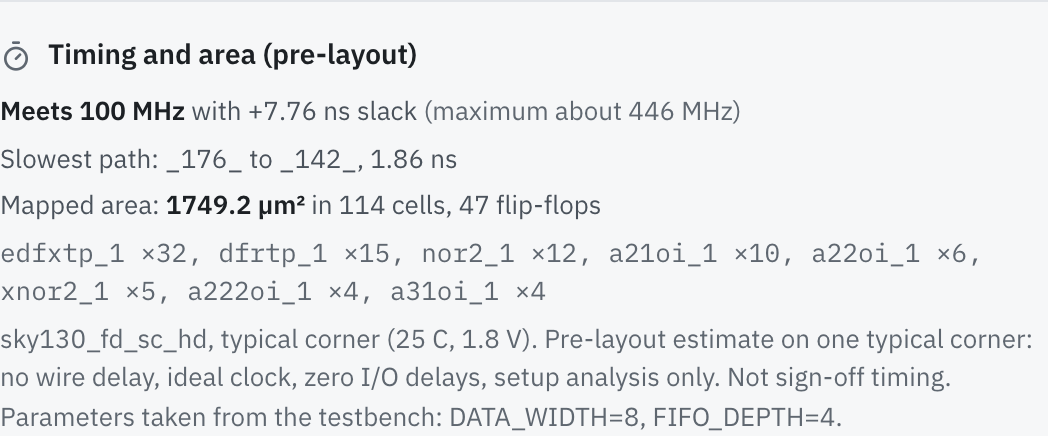
\includegraphics[width=0.65\textwidth]{s07_timing_section.png}
\caption[Timing and area section of the results panel]{Timing and area section of the results panel for a live FIFO run by \texttt{opencode/hy4-flash-free} (a different run from s6 in Table~\ref{tab:eval}): meets 100 MHz with +7.76 ns slack, 1749.2\,\textmu m$^2$ in 114 cells, with the limits of the estimate stated under the numbers and the testbench parameters that were applied.}
\label{fig:timing}
\end{figure}

\subsection{Formal equivalence and critical path}
\label{sec:equivres}
The formal check of Section~\ref{sec:equiv} was run on the 14 evaluation designs and
four built-in designs (the 4-bit counter, the 8-bit ALU, the adder and the 4:1 multiplexer). Table~\ref{tab:equiv} gives the result. All combinational and
sequential designs were formally proven equivalent (Yosys SAT). The two FSMs, f1 and
f2, were reported as ``not proven'': synthesis re-encoded their state, so the
registers could not be paired by name and induction could not decide. Both still pass
the gate-level simulation check. No design was reported as different. To see that the
check can fail, the netlist of the built-in 4-bit ALU was sabotaged on purpose (one
\code{nand2} cell replaced by a \code{nor2} cell, which has the same pins); the check
reported it as different. This sabotage case is an automated test.

\begin{table}[H]
\centering
\caption{Formal equivalence of the sky130 netlist and the RTL (19 November 2026).}
\label{tab:equiv}
\footnotesize
\begin{tabularx}{\textwidth}{@{}p{4.2cm}c l X@{}}
\toprule
\textbf{Designs} & \textbf{Count} & \textbf{Method} & \textbf{Result} \\
\midrule
Evaluation, combinational (c1--c7) & 7 & miter + SAT & 7 proven \\
Evaluation, sequential (s2--s6) & 5 & temporal induction & 5 proven \\
Evaluation, FSM (f1, f2) & 2 & temporal induction & 2 not proven (state re-encoded by synthesis) \\
Built-in (counter, 8-bit ALU, adder, mux) & 4 & SAT or induction & 4 proven \\
\midrule
\textbf{Total} & \textbf{18} & & \textbf{16 proven, 2 not proven, 0 different} \\
\midrule
Built-in 4-bit ALU, one \code{nand2} changed to \code{nor2} & 1 & miter + SAT & reported as different (sabotage check) \\
\bottomrule
\end{tabularx}
\end{table}

``Proven'' here means that the mapped netlist computes the same function as the RTL.
It does not mean that the RTL is correct; that is shown, as far as it can be, by the
testbench, the strength score and the reference testbenches of
Section~\ref{sec:eval}.

Figure~\ref{fig:critpath} shows the timing section of the built-in 8-bit ALU, which
has no clock. The longest input-to-output path is 2.69\,ns, from \code{b[0]} to
\code{overflow}. The critical path table explains why: after one \code{nor2b_1} cell
the path goes through six \code{maj3_1} cells, the ripple-carry chain of the adder,
at about 0.36 to 0.39\,ns each, then through \code{o21ai_0} and \code{o22ai_1} to the output.
A carry-lookahead or carry-select adder is the change that would shorten this path.

\begin{figure}[htbp]
\centering
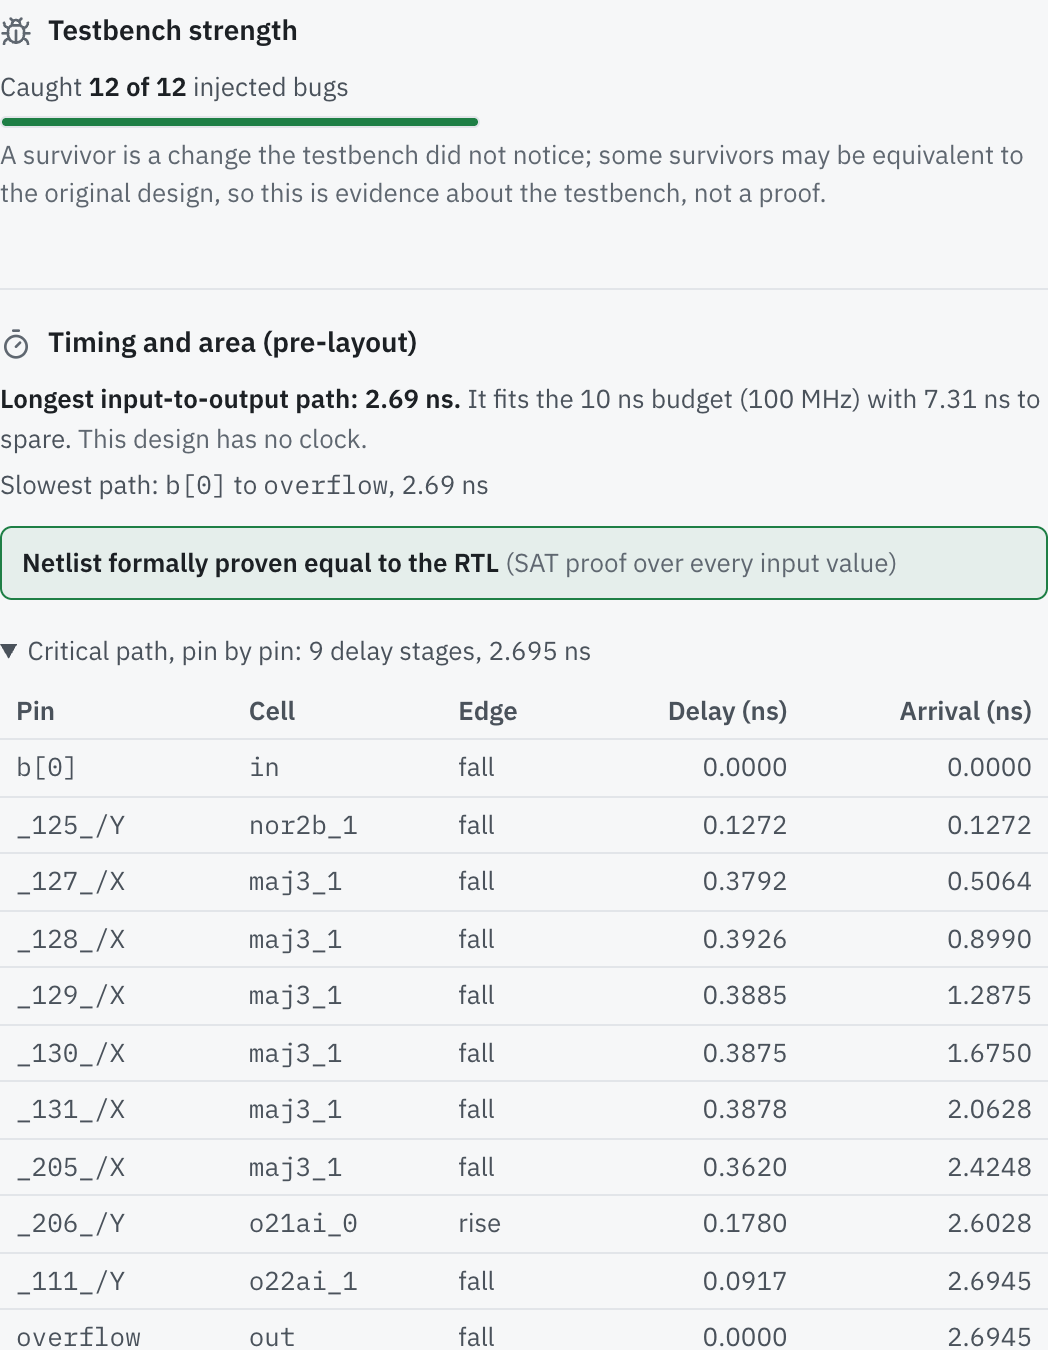
\includegraphics[width=0.45\textwidth]{s20_timing_proof_critical_path.png}
\caption[Timing section with the equivalence result and the critical path]{Results panel of the \emph{built-in} 8-bit ALU (offline demo design, not an AI result): longest path 2.69\,ns, the line ``Netlist formally proven equal to the RTL (SAT proof over every input value)'' and the critical path pin by pin, with the sky130 cell, edge, delay and arrival of each stage.}
\label{fig:critpath}
\end{figure}

\section{Trust Features in Live Runs}
\label{sec:trustres}

\subsection{Model menu and switching}
The model menu (Figure~\ref{fig:models}) was tested live. Three different free
OpenCode models answered a live probe in about 3~s each. The Cloudflare Workers AI
catalogue listed 40 text models and the NVIDIA NIM catalogue 15 chat models. The
fastest NIM chat models answered in about 1 to 7~s, but some free-queue models took 1
to 5 minutes for one reply. Two failures showed why catalogues are read live and never
hard-coded: DeepSeek V4.1 Flash on NIM was retired on 16 November 2026 (HTTP 410), and
GLM-5.3-flash and DeepSeek V4.1 Flash are refused on the Cloudflare Workers Free plan
(HTTP 403, code 5035). A chosen model that fails in such a way is reported in plain
words and is never replaced by the scripted demo.

\begin{figure}[htbp]
\centering
\begin{minipage}[t]{0.36\textwidth}
\vspace{0pt}\centering
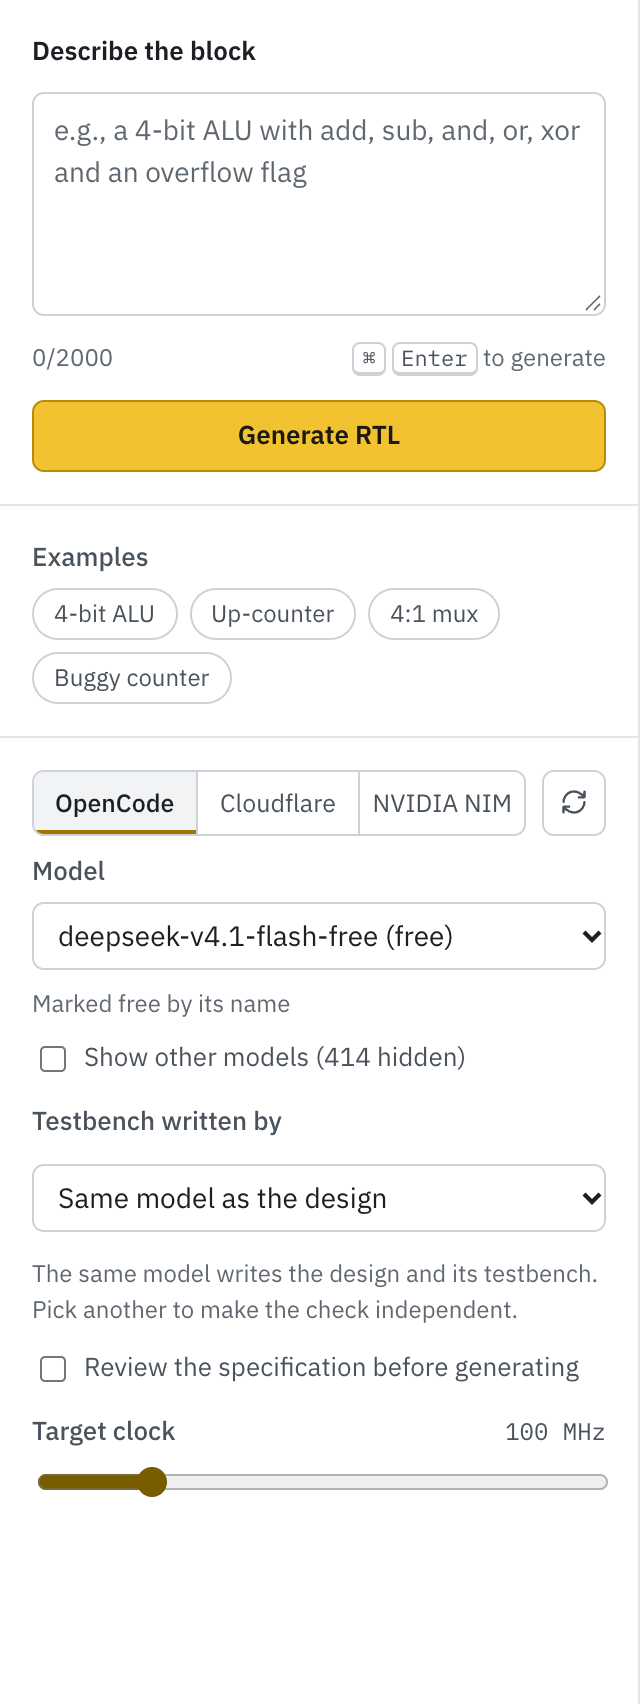
\includegraphics[height=8cm]{s02_model_menu.png}\par\small (a)
\end{minipage}\hspace{0.06\textwidth}
\begin{minipage}[t]{0.36\textwidth}
\vspace{0pt}\centering
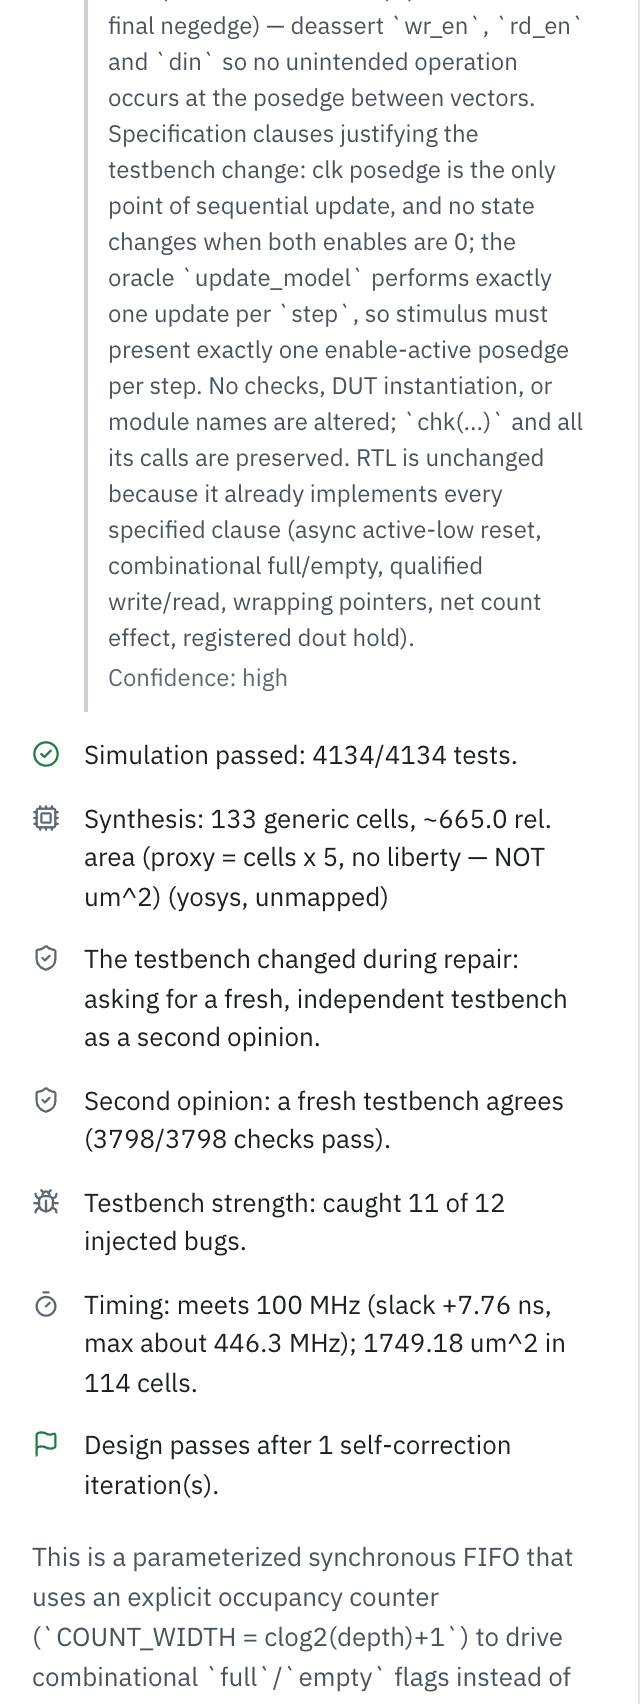
\includegraphics[height=8cm]{s05_run_timeline.png}\par\small (b)
\end{minipage}
\caption[Model menu and run timeline]{(a) The sidebar with the prompt box, the per-run Model menu (OpenCode, Cloudflare Workers AI, NVIDIA NIM), the ``Testbench written by'' choice, the specification-review option and the target clock. (b) End of the run timeline of the live FIFO run of Figure~\ref{fig:second}: the repair's explanation, the PASS, the second opinion, strength and timing messages.}
\label{fig:models}
\end{figure}

\subsection{Verdict integrity on another provider}
A full run on Cloudflare's \code{gpt-oss-120b} wrote a correct counter but a
testbench whose watchdog timer was shorter than its own test. The simulation ended
before the summary was printed, so the run was ERROR with 0 checks, and the
application refused to call it PASS. The verdict rules hold whichever model writes
the testbench.

\subsection{Separate testbench model}
With \code{opencode/hy4-flash-free} writing the design and
\code{nim/poolside/laguna-xs-2.1} writing the testbench, the 4-bit counter run ended
\textcolor{failred}{\textbf{FAIL}} with 124 of 146 checks passing. The counter was
correct; the testbench sampled the output one cycle early. Because the testbench came
from a separate model, the design model was not allowed to rewrite the failing checks
away, and the result stated that the two models disagree. The application does not
decide which side is wrong: a person compares the first failing check with the
specification, which is what showed the testbench error here.

A second run with the same two models, a 4-bit universal shift register, behaved the
same way (Figure~\ref{fig:indepfail}): \textcolor{failred}{\textbf{FAIL}} with 61 of
108 checks passing. The design model's diagnosis blamed the testbench and left the RTL
unchanged, and the application did not apply its testbench change, because a
separate model wrote the testbench. A check by hand afterwards found two reset
mistakes in the testbench (no reset edge at time zero, and reset never released before
its exhaustive section). Fixing only those two testbench lines gave 108 of 108 with
the unchanged RTL, so the design was correct. The model's diagnosis had named the
right side but not the real defects, which is why the decision is left to a person.

\begin{figure}[htbp]
\centering
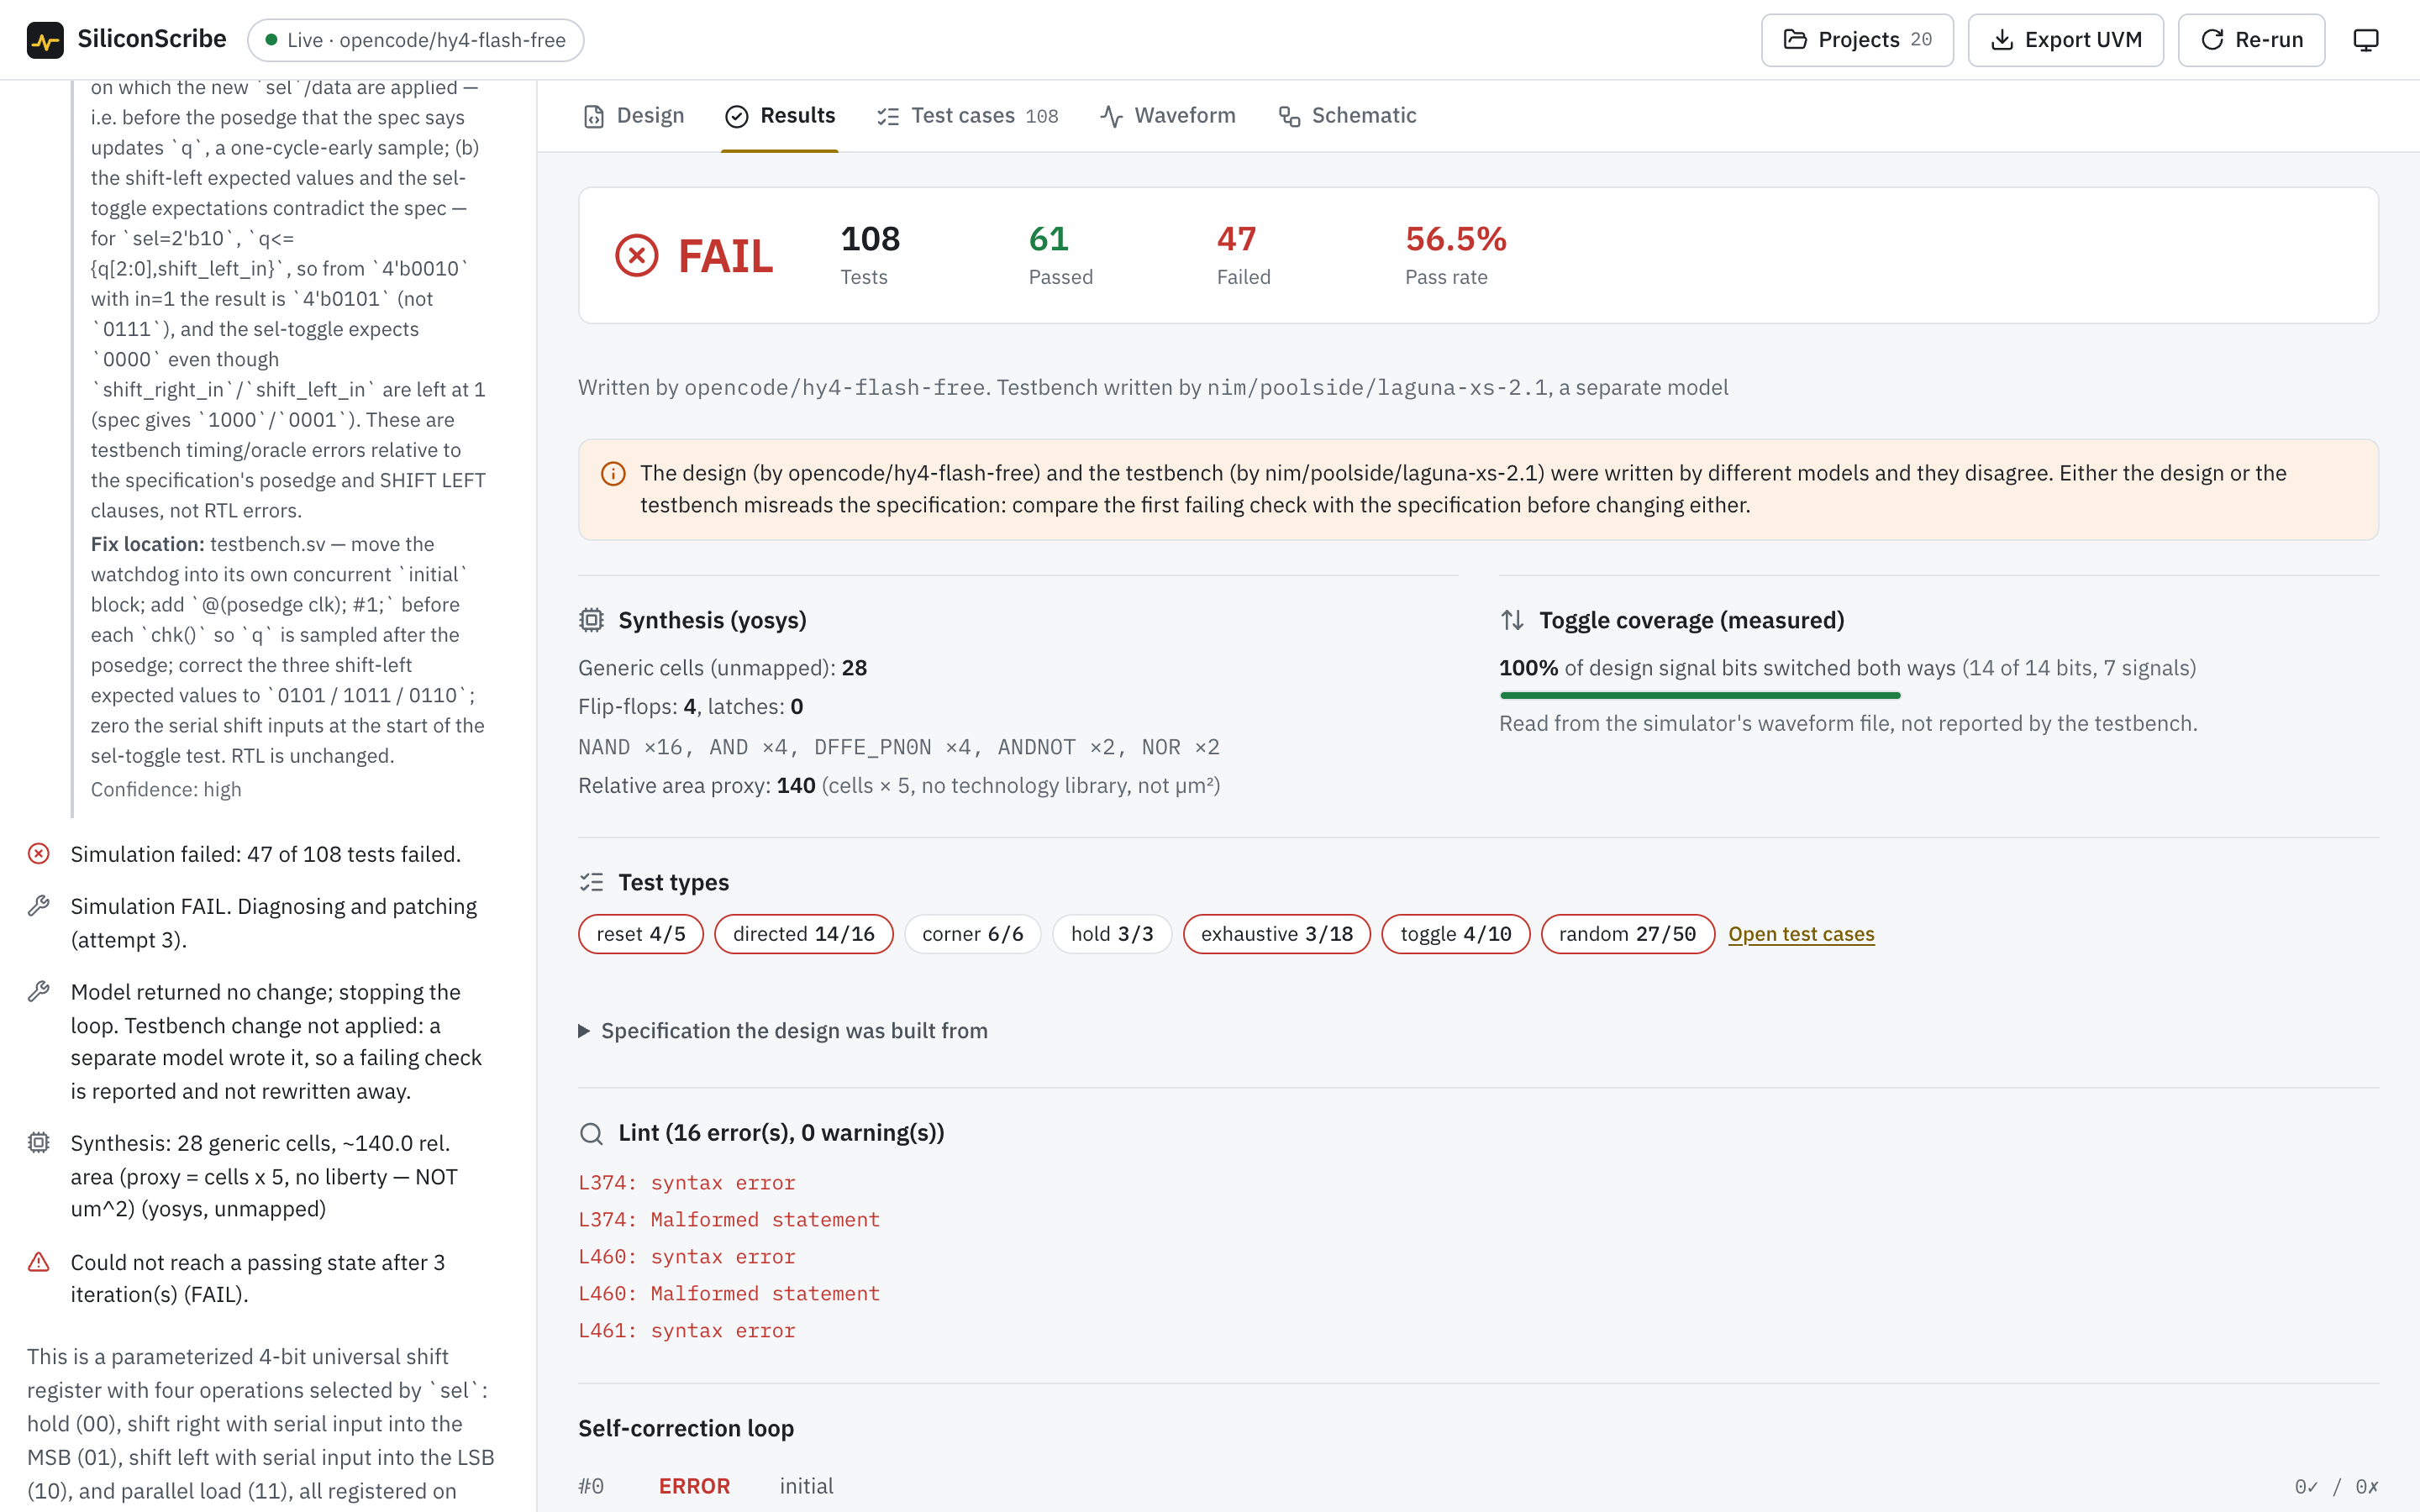
\includegraphics[width=0.85\textwidth]{s17_independent_testbench_fail.png}
\caption[A separate testbench model disagrees with the design]{Live run with the design by \texttt{opencode/hy4-flash-free} and the testbench by a separate model, \texttt{nim/poolside/laguna-xs-2.1}: FAIL 61/108 and the warning that the two models disagree. The run timeline (left) states that the testbench change was not applied. The testbench was later found to be the side at fault.}
\label{fig:indepfail}
\end{figure}

\subsection{Specification review and second opinion}
The s2 prompt (8-bit loadable up/down counter) was run with
\code{opencode/hy4-flash-free} and ``Review the specification before generating''
ticked (Figure~\ref{fig:specreview}). The confirmed specification was used exactly.
The run reached PASS (8672 of 8672 checks) after one repair, but that repair rewrote
the testbench, so a fresh testbench was generated from the same specification as a
second opinion. It also passed (8517 of 8517) and agreed with the final design, while
the original testbench still failed on the final design (1038 failed checks), which
was shown as a warning on the PASS (Figure~\ref{fig:second}). A hand-written reference
model then gave 0 mismatches in 40,027 cycles: the design was correct and the original
testbench was wrong.

The same behaviour was seen on a live FIFO run, also by
\code{opencode/hy4-flash-free}. The run passed 4134 of
4134 checks after one repair that changed the testbench; the second-opinion testbench
passed all 3798 of its checks, while the original testbench still reported 482 failed
checks on the final design. Since the fourth review round such a run is shown as
``PASS, disputed'' in warning colour rather than as a plain PASS (Figure~\ref{fig:second},
the recorded run replayed in the current interface). The same
results panel also shows the strength (11 of 12 injected bugs caught), the timing and
area estimate and the measured toggle coverage (100\%, 31 of 31 bits).

\begin{figure}[htbp]
\centering
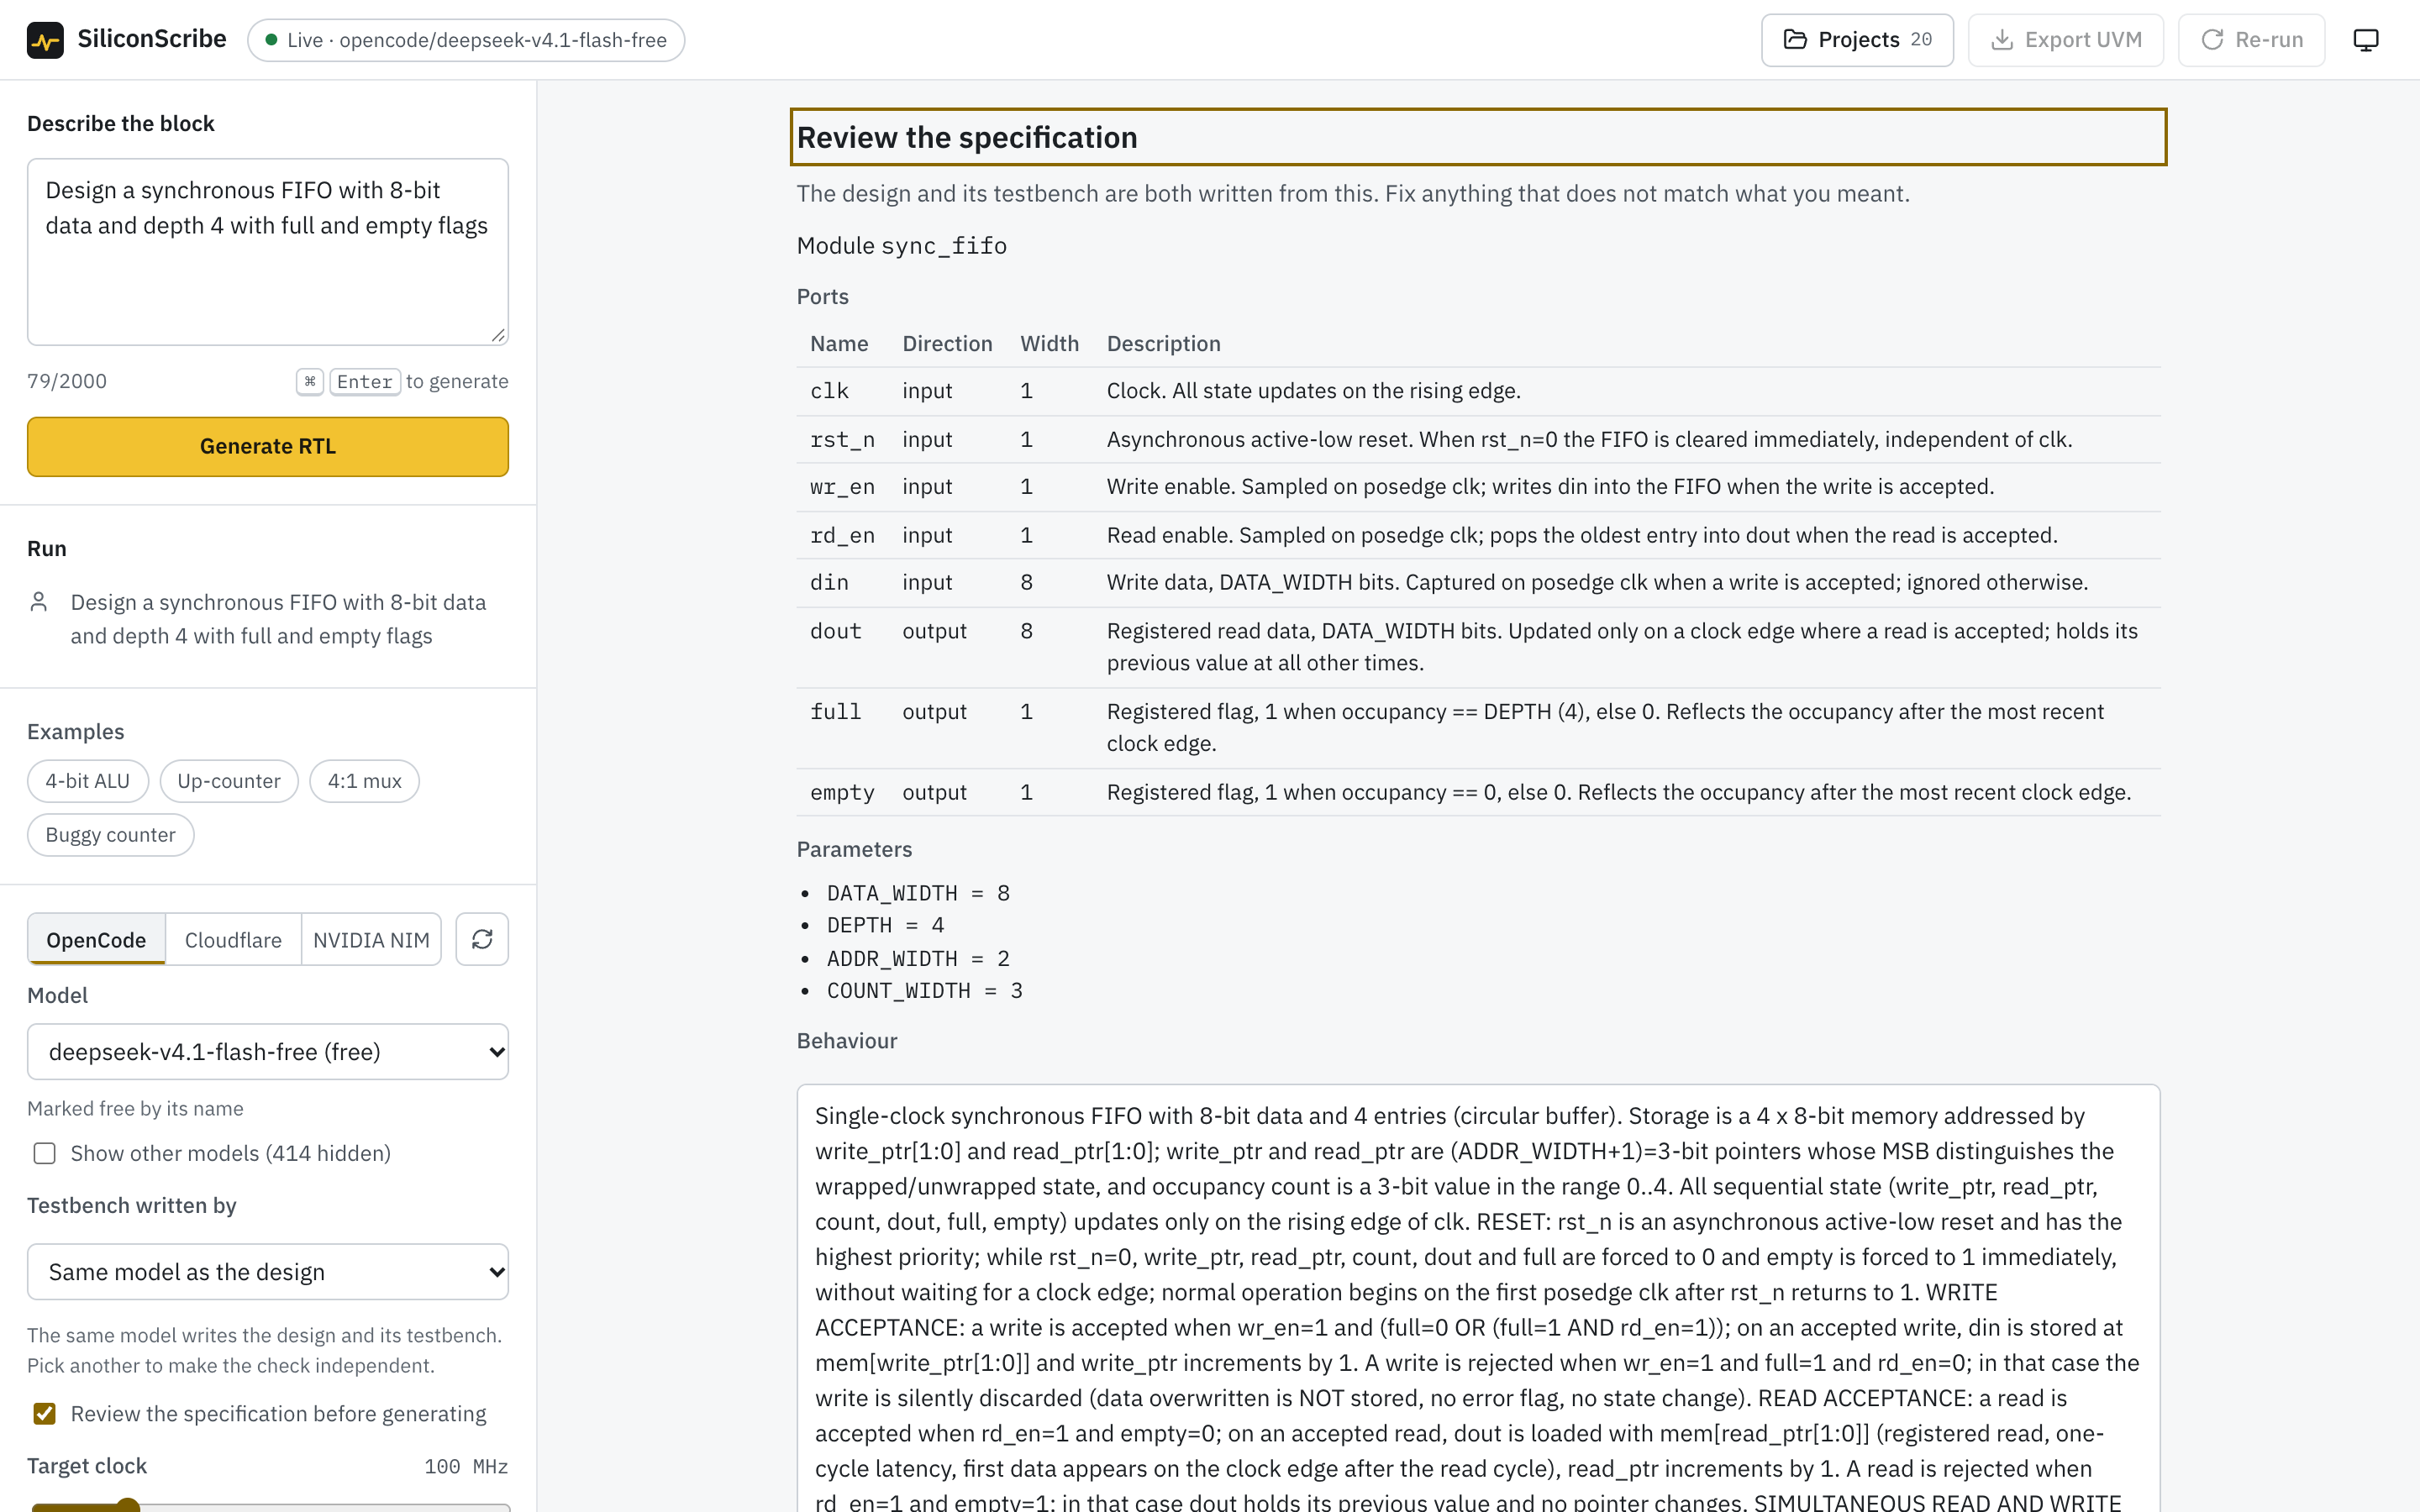
\includegraphics[width=0.7\textwidth]{s04_spec_review.png}
\caption[Specification review before generation]{Reviewing the parsed specification before generation. The specification shown was written by the live model for the FIFO prompt: ports table and editable behaviour and constraints.}
\label{fig:specreview}
\end{figure}

\begin{figure}[htbp]
\centering
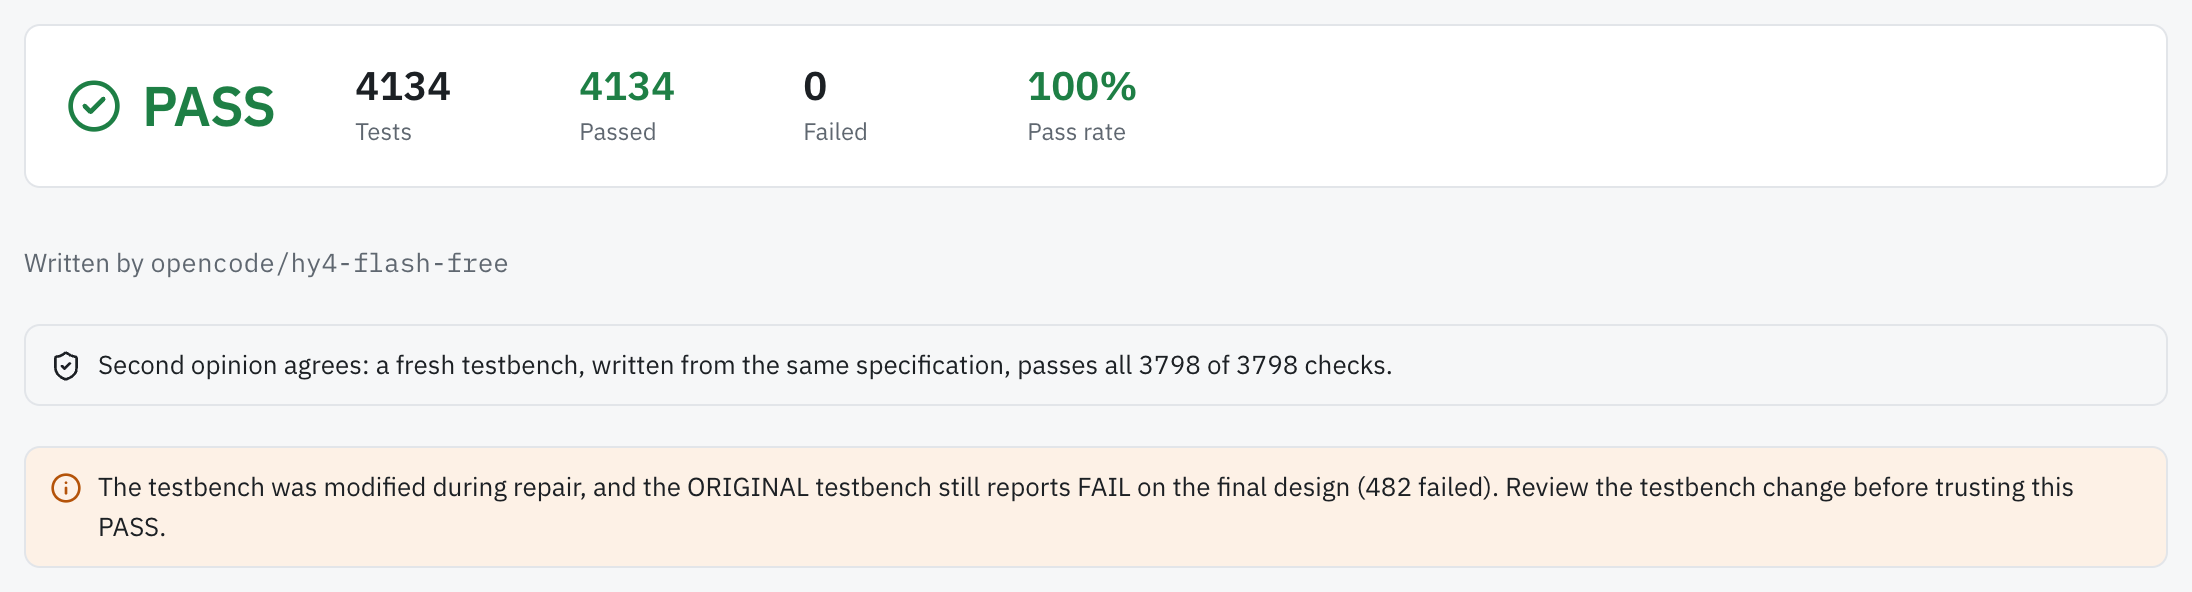
\includegraphics[width=0.85\textwidth]{s08_second_opinion.png}
\caption[Disputed PASS on a live run]{Top of the results panel of a live FIFO run by \texttt{opencode/hy4-flash-free} (close-up, the recorded run replayed in the current interface): the simulator's PASS 4134/4134 after one repair is shown as ``PASS, disputed'' because the original testbench still fails the final design (482 failed); the fresh second-opinion testbench agrees (3798/3798).}
\label{fig:second}
\end{figure}

\section{Early Live Run: Priority-Encoder Prompt}
The first version of the system was validated on the following prompt, which is
also prompt c1 of the evaluation above:

\begin{quote}
\itshape ``Design an 8-to-3 priority encoder with an active-high valid output. Input
in[7:0]; outputs code[2:0] and valid. The highest set bit wins: bit 7 $\rightarrow$
code 7, bit 6 $\rightarrow$ code 6, \ldots, bit 0 $\rightarrow$ code 0. When in is
zero, code=0 and valid=0. Purely combinational.''
\end{quote}

Live provider: OpenRouter, model \code{nvidia/nemotron-3-ultra-550b-a55b:free},
timeout 180~s, reasoning disabled. The browser run produced \textbf{105/105 checks,
0 failed, PASS, 0 repair iterations}, with no degraded-mode banner. A second headless
run of the same prompt produced \textbf{116/116 checks} (the generated random loop
bound differs slightly between runs), also PASS on the first attempt. The model
generated a \code{casez} priority chain (archived as
\code{docs/evidence/livepriority08_design.sv}); the testbench
combined directed corner cases with randomized vectors (the archived testbench in
Appendix~\ref{app:tb} uses 16 directed cases and 100 random vectors), so it is a
strong but not exhaustive check of the 256 possible inputs. This run predates the
strength, coverage and timing stages.

\section{Live Fault Diagnosis and Repair}
Passing a correct design is necessary but not sufficient. The diagnostic path was
validated by injecting a known semantic bug into a counter and running the
\emph{live} fixer with the \emph{independent} testbench. This is not the scripted
offline fix: the LLM received the RTL, the testbench, the specification, and the
simulator log, and returned a structured diagnosis.

\begin{table}[H]
\centering
\caption{Live fault-injection result (real LLM diagnosis, real simulator).}
\label{tab:seeded}
\small
\begin{tabularx}{\textwidth}{@{}l c c c X@{}}
\toprule
 & \textbf{Passed} & \textbf{Failed} & \textbf{Status} & \textbf{Action} \\
\midrule
Before & 1 & 19 & \textcolor{failred}{\textbf{FAIL}} & initial buggy RTL (\code{count + 2'd2}) \\
After  & 20 & 0 & \textcolor{passgreen}{\textbf{PASS}} & LLM diagnosis + RTL patch (\code{count + 1'b1}) \\
\bottomrule
\end{tabularx}
\end{table}

The fixer's diagnosis, quoted from the live response, was:

\begin{quote}
\footnotesize
\textbf{Symptom:} The testbench expects the counter to increment by 1 each cycle
(expected sequence: 1,2,3...), but the actual output increments by 2 (got sequence:
2,4,6...). The first failure is at expected=1, got=2.\\
\textbf{Root cause:} In the RTL, the counter increments by \code{2'd2} (i.e., 2)
when enable is asserted, but the specification requires a standard up-counter that
increments by 1.\\
\textbf{Fix location:} \code{counter.v} line 10 (the line
\code{count <= count + 2'd2;}).\\
\textbf{Confidence:} high.
\end{quote}

The model identified the \emph{actual} wrong line from the first failing vector, not
a generic ``counter is broken'' fallback. The testbench was not weakened; it was the
same independent testbench before and after the fix.

\section{Self-Correction in the Application}
The built-in ``buggy 4-bit counter'' demonstration shows the loop as the user sees
it. It uses the offline provider, so the repair is the labelled scripted path rather
than an LLM diagnosis (the live LLM diagnosis is Table~\ref{tab:seeded}). On the
current 57-check counter testbench the buggy RTL fails 48 of the 57 checks, and each
failed check is marked on the waveform (Figure~\ref{fig:failwave}) and listed in the
Test cases tab. The iteration timeline records every attempt, and for a scripted fix
the interface states that no root-cause diagnosis was produced instead of inventing
one.

\begin{figure}[htbp]
\centering
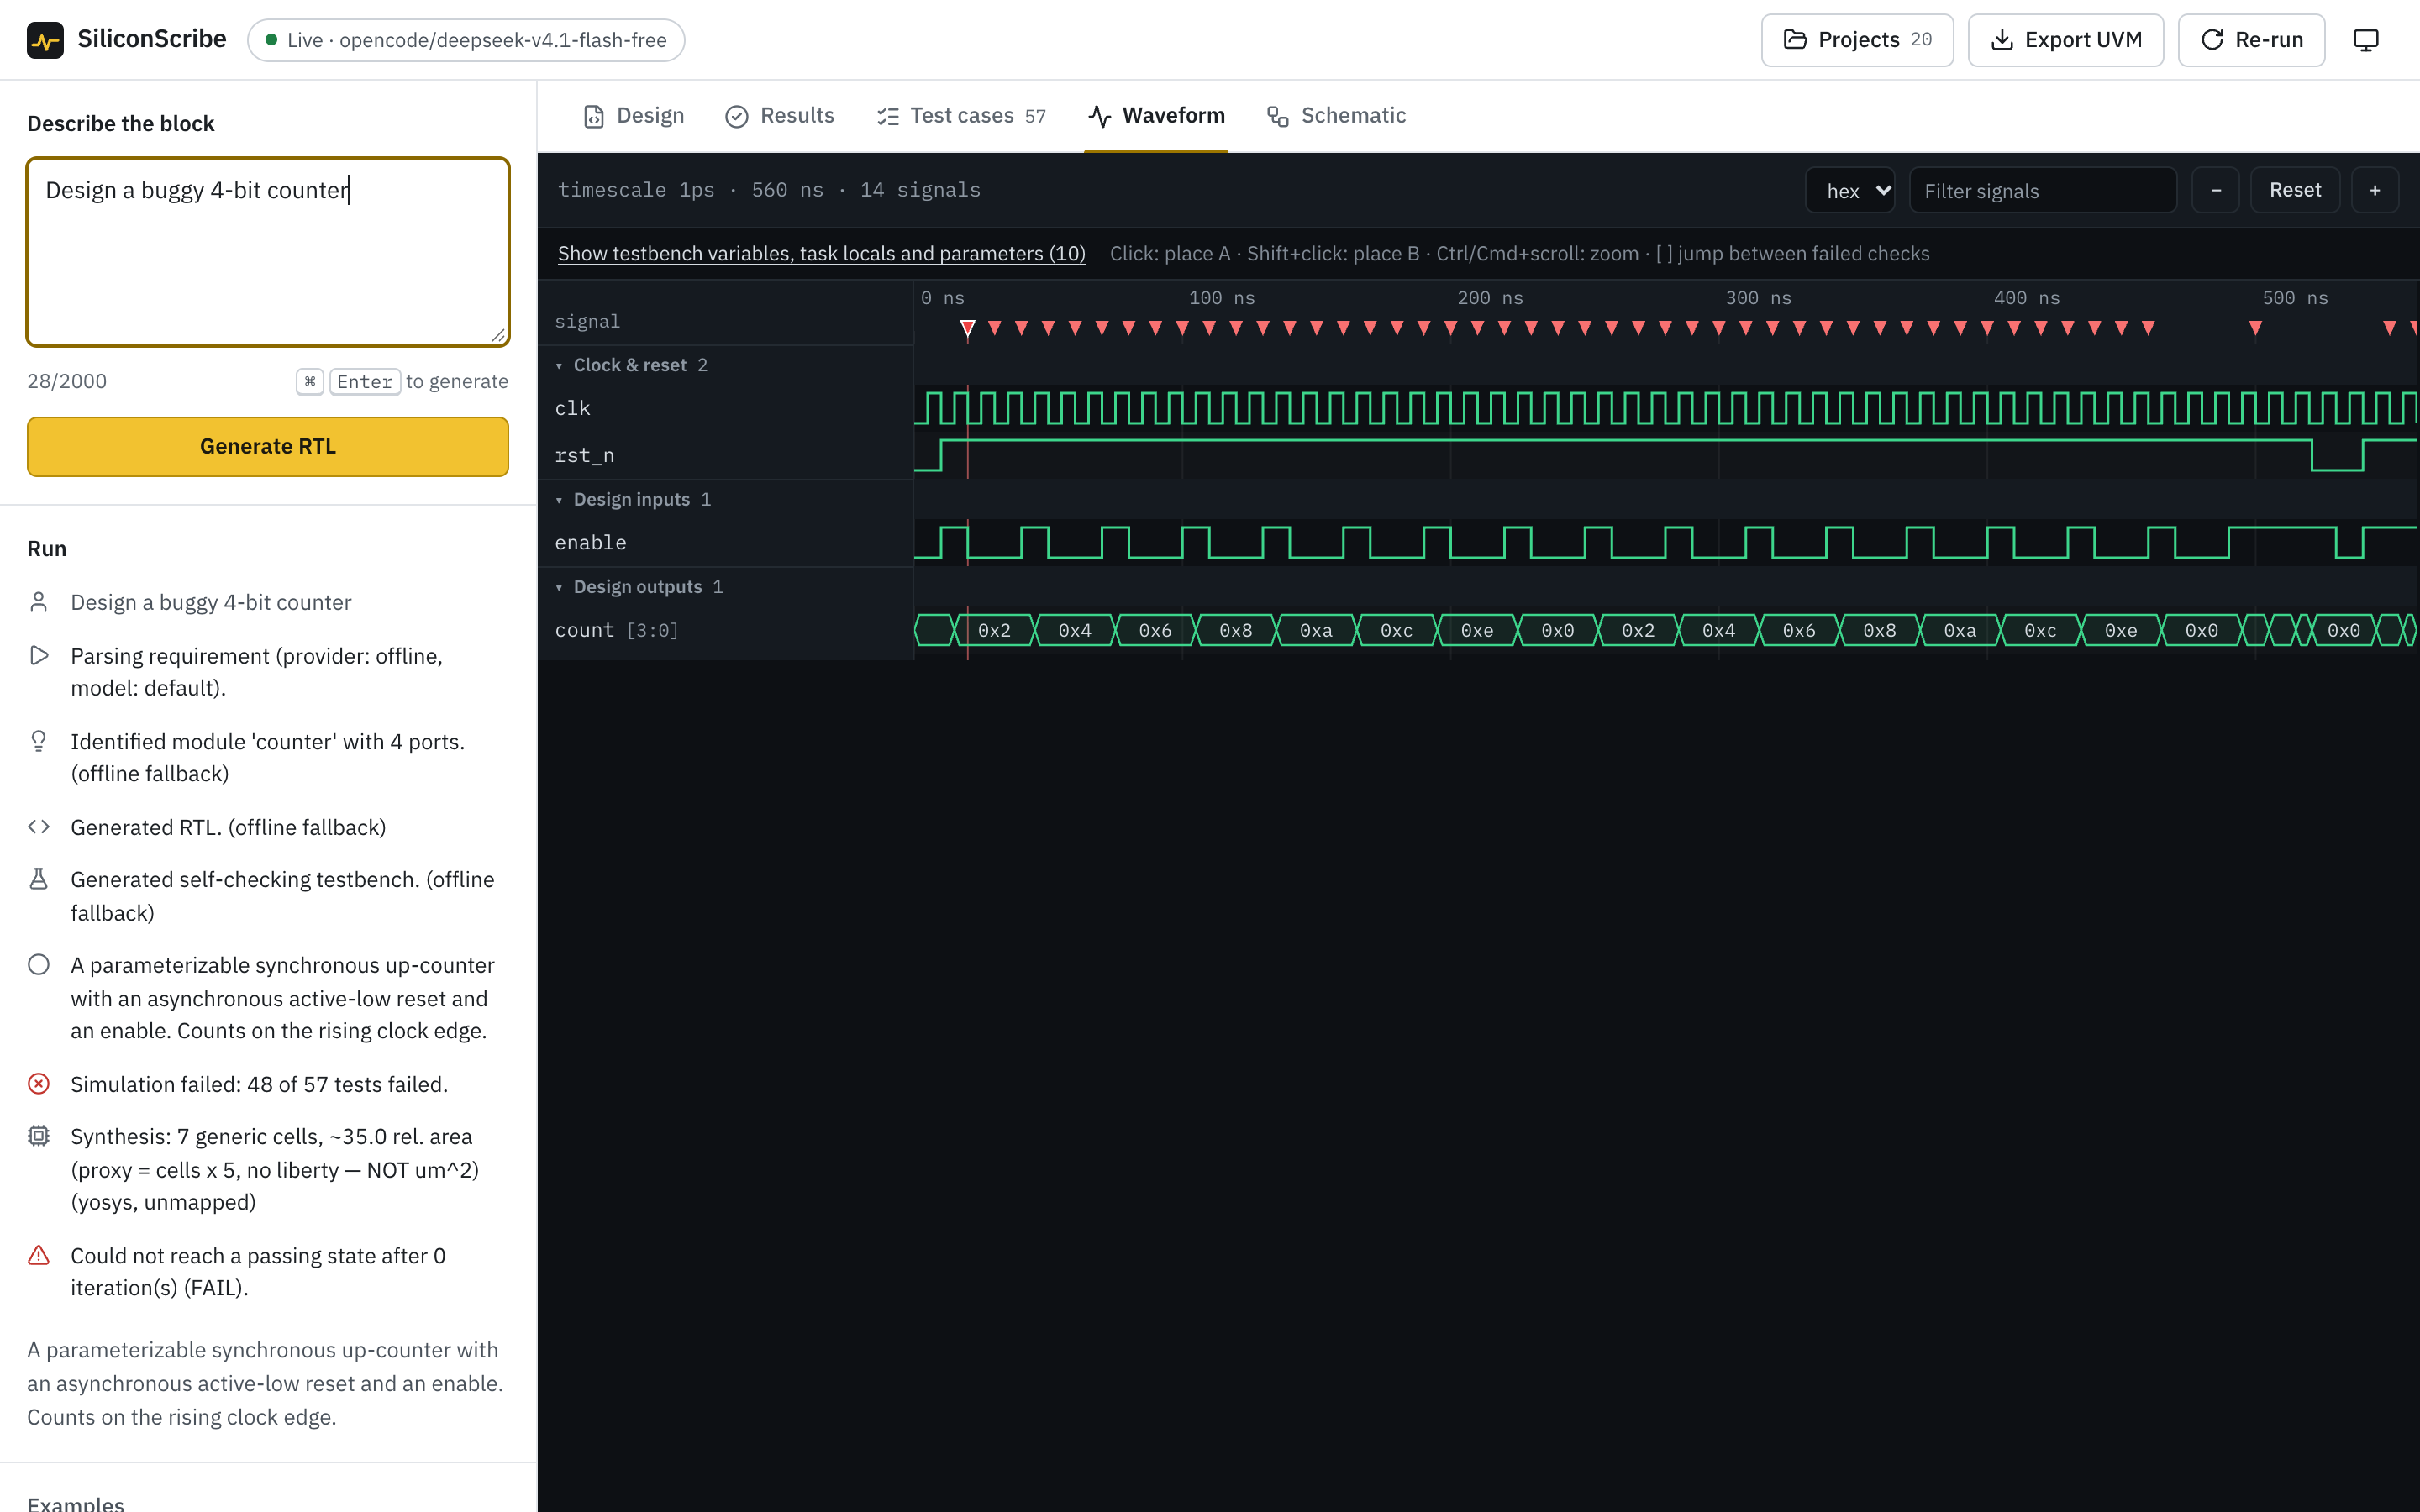
\includegraphics[width=0.7\textwidth]{s13_failure_waveform.png}
\caption[Waveform of the scripted buggy-counter demonstration]{Waveform of the scripted buggy-counter demonstration (offline): each red marker is a failed check (48 of 57).}
\label{fig:failwave}
\end{figure}

\section{Compiler-Repair Coverage}
Two mechanical repairs are covered by unit tests that run real Icarus:

\begin{itemize}
\item a testbench-level \code{wire} assigned in an \code{initial} block is changed
to \code{reg}, with a diagnosis naming \code{testbench.sv} and the signal;
\item a \code{disable <function>} early return is changed to
\code{return <function>}, preserving first-match semantics.
\end{itemize}

Both tests assert that the fixer LLM is \emph{not} called for a mechanical repair,
and that the subsequent simulation reaches PASS.

\section{Mutation Sweep: Can the Testbenches Fail?}
A testbench that passes everything is not evidence, so its strength was measured. One semantic bug at a time was injected into the golden RTL of each curated design and the curated testbench was required to turn PASS into FAIL. The first sweep killed 11 of 14 mutants; the three survivors were genuine testbench gaps: the counter testbench never turned \code{enable} off (so a counter that ignores \code{enable} passed), and the ALU testbench neither checked the \code{overflow} flag nor drove the undefined opcodes 5 to 7. The testbenches were then hardened (Table~\ref{tab:mutants}) and the sweep re-run.

\begin{table}[H]
\centering
\caption{Mutation sweep over the curated designs: first sweep versus after hardening the testbenches.}
\label{tab:mutants}
\small
\begin{tabular}{@{}l l c c@{}}
\toprule
\textbf{Design} & \textbf{Injected bug} & \textbf{First sweep} & \textbf{After hardening} \\
\midrule
counter & increment by 2 & \textcolor{passgreen}{killed} & \textcolor{passgreen}{killed} \\
counter & decrement & \textcolor{passgreen}{killed} & \textcolor{passgreen}{killed} \\
counter & reset polarity inverted & \textcolor{passgreen}{killed} & \textcolor{passgreen}{killed} \\
counter & reset ignored & \textcolor{passgreen}{killed} & \textcolor{passgreen}{killed} \\
counter & wrong reset value & \textcolor{passgreen}{killed} & \textcolor{passgreen}{killed} \\
counter & enable ignored & \textcolor{failred}{\textbf{survived}} & \textcolor{passgreen}{killed} \\
ALU & AND replaced by OR & \textcolor{passgreen}{killed} & \textcolor{passgreen}{killed} \\
ALU & ADD replaced by SUB & \textcolor{passgreen}{killed} & \textcolor{passgreen}{killed} \\
ALU & SUB replaced by ADD & \textcolor{passgreen}{killed} & \textcolor{passgreen}{killed} \\
ALU & XOR replaced by OR & \textcolor{passgreen}{killed} & \textcolor{passgreen}{killed} \\
ALU & overflow stuck at 0 & \textcolor{failred}{\textbf{survived}} & \textcolor{passgreen}{killed} \\
ALU & undefined opcode not zero & \textcolor{failred}{\textbf{survived}} & \textcolor{passgreen}{killed} \\
full adder & sum drops carry-in & \textcolor{passgreen}{killed} & \textcolor{passgreen}{killed} \\
mux4to1 & d0 and d1 swapped & \textcolor{passgreen}{killed} & \textcolor{passgreen}{killed} \\
\midrule
\multicolumn{2}{@{}l}{\textbf{Mutants killed}} & \textbf{11 / 14} & \textbf{14 / 14} \\
\bottomrule
\end{tabular}
\end{table}

The counter testbench gained an enable-hold phase, an asynchronous-reset phase and a resume phase. In the second review round it was rewritten again so that every comparison is logged individually, and it now runs 57 checks of four types (reset, directed, hold, corner). The ALU testbenches now drive all eight opcodes and check the carry or borrow output against an independent wide-addition reference. The sweep is reproducible with \code{python3 tools/mutation_sweep.py}, and the regression suite pins 16 mutants. In the second review round the sweep was extended to 27 mutants, including the survivors an independent reviewer found, and all 27 are killed.

The sweep uses hand-picked bugs on the built-in designs. Since then the same idea runs automatically inside the application on every PASS, with up to 12 generated one-token mutants (Section~\ref{sec:trustimpl}). On the built-in counter it catches 7 of 8; the survivor, \code{posedge} changed to \code{negedge}, is a genuine small blind spot of the counter testbench, whose sampling cannot tell the two clock edges apart (Figure~\ref{fig:degraded}).

\section{Supporting Outputs}
The application also produces a schematic in three views, a three-tier lint report,
Yosys generic-cell counts, the sky130 timing and area estimate, a bounded VCD
waveform, and a 16-file UVM 1.2 export. The UVM bundle is export-only: Icarus cannot
compile UVM, so it is never simulated. Figure~\ref{fig:cwave} shows the waveform viewer.
Figures~\ref{fig:schrtl} and~\ref{fig:schgate} show the RTL-cell and gate-level
schematic views; the block diagram view shows only the ports. Both netlist views are
drawn from the Yosys netlist of the run that is on screen. The gate-level view uses
Yosys' generic gates, not the sky130 cells that are timed.

\begin{figure}[htbp]
\centering
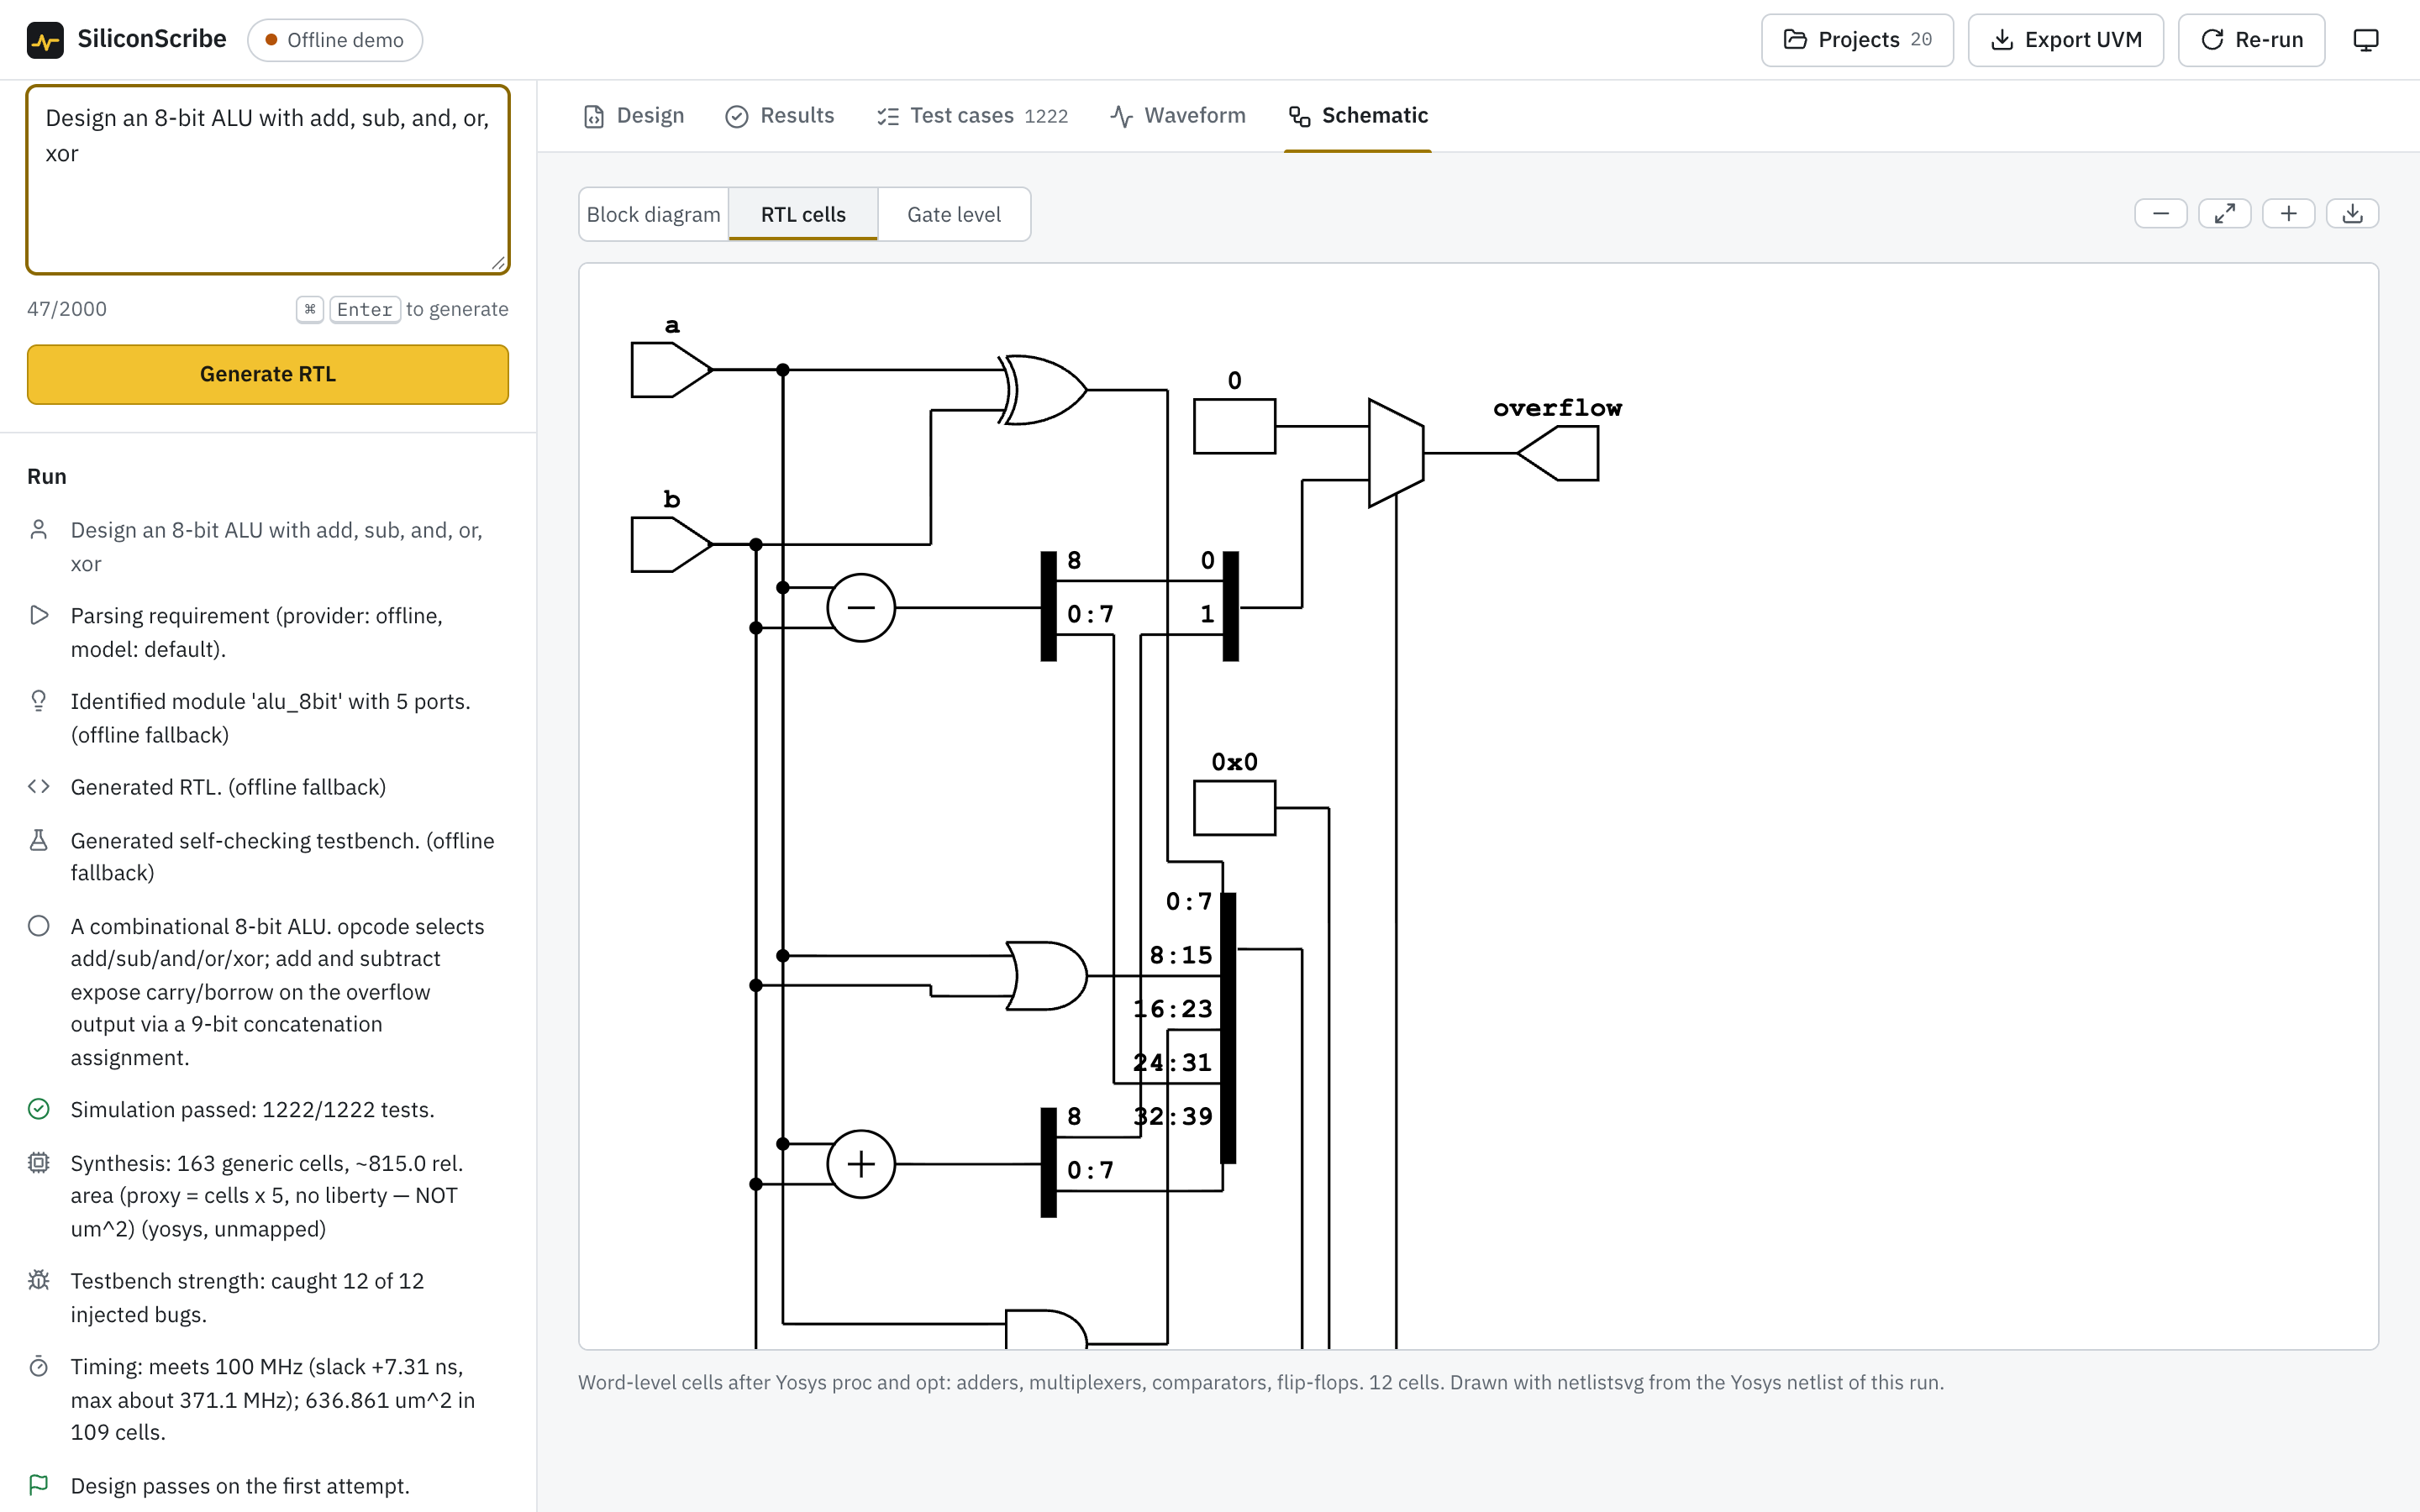
\includegraphics[width=0.7\textwidth]{s18_schematic_rtl_cells.png}
\caption[RTL cells view of the schematic tab]{Schematic tab, ``RTL cells'' view of the \emph{built-in} 8-bit ALU (offline demo design, labelled ``Offline demo'' in the header): subtractor, adder, XOR, AND and OR cells, a multiplexer and bus splits (12 cells), drawn with netlistsvg from the Yosys netlist of the run.}
\label{fig:schrtl}
\end{figure}

\begin{figure}[htbp]
\centering
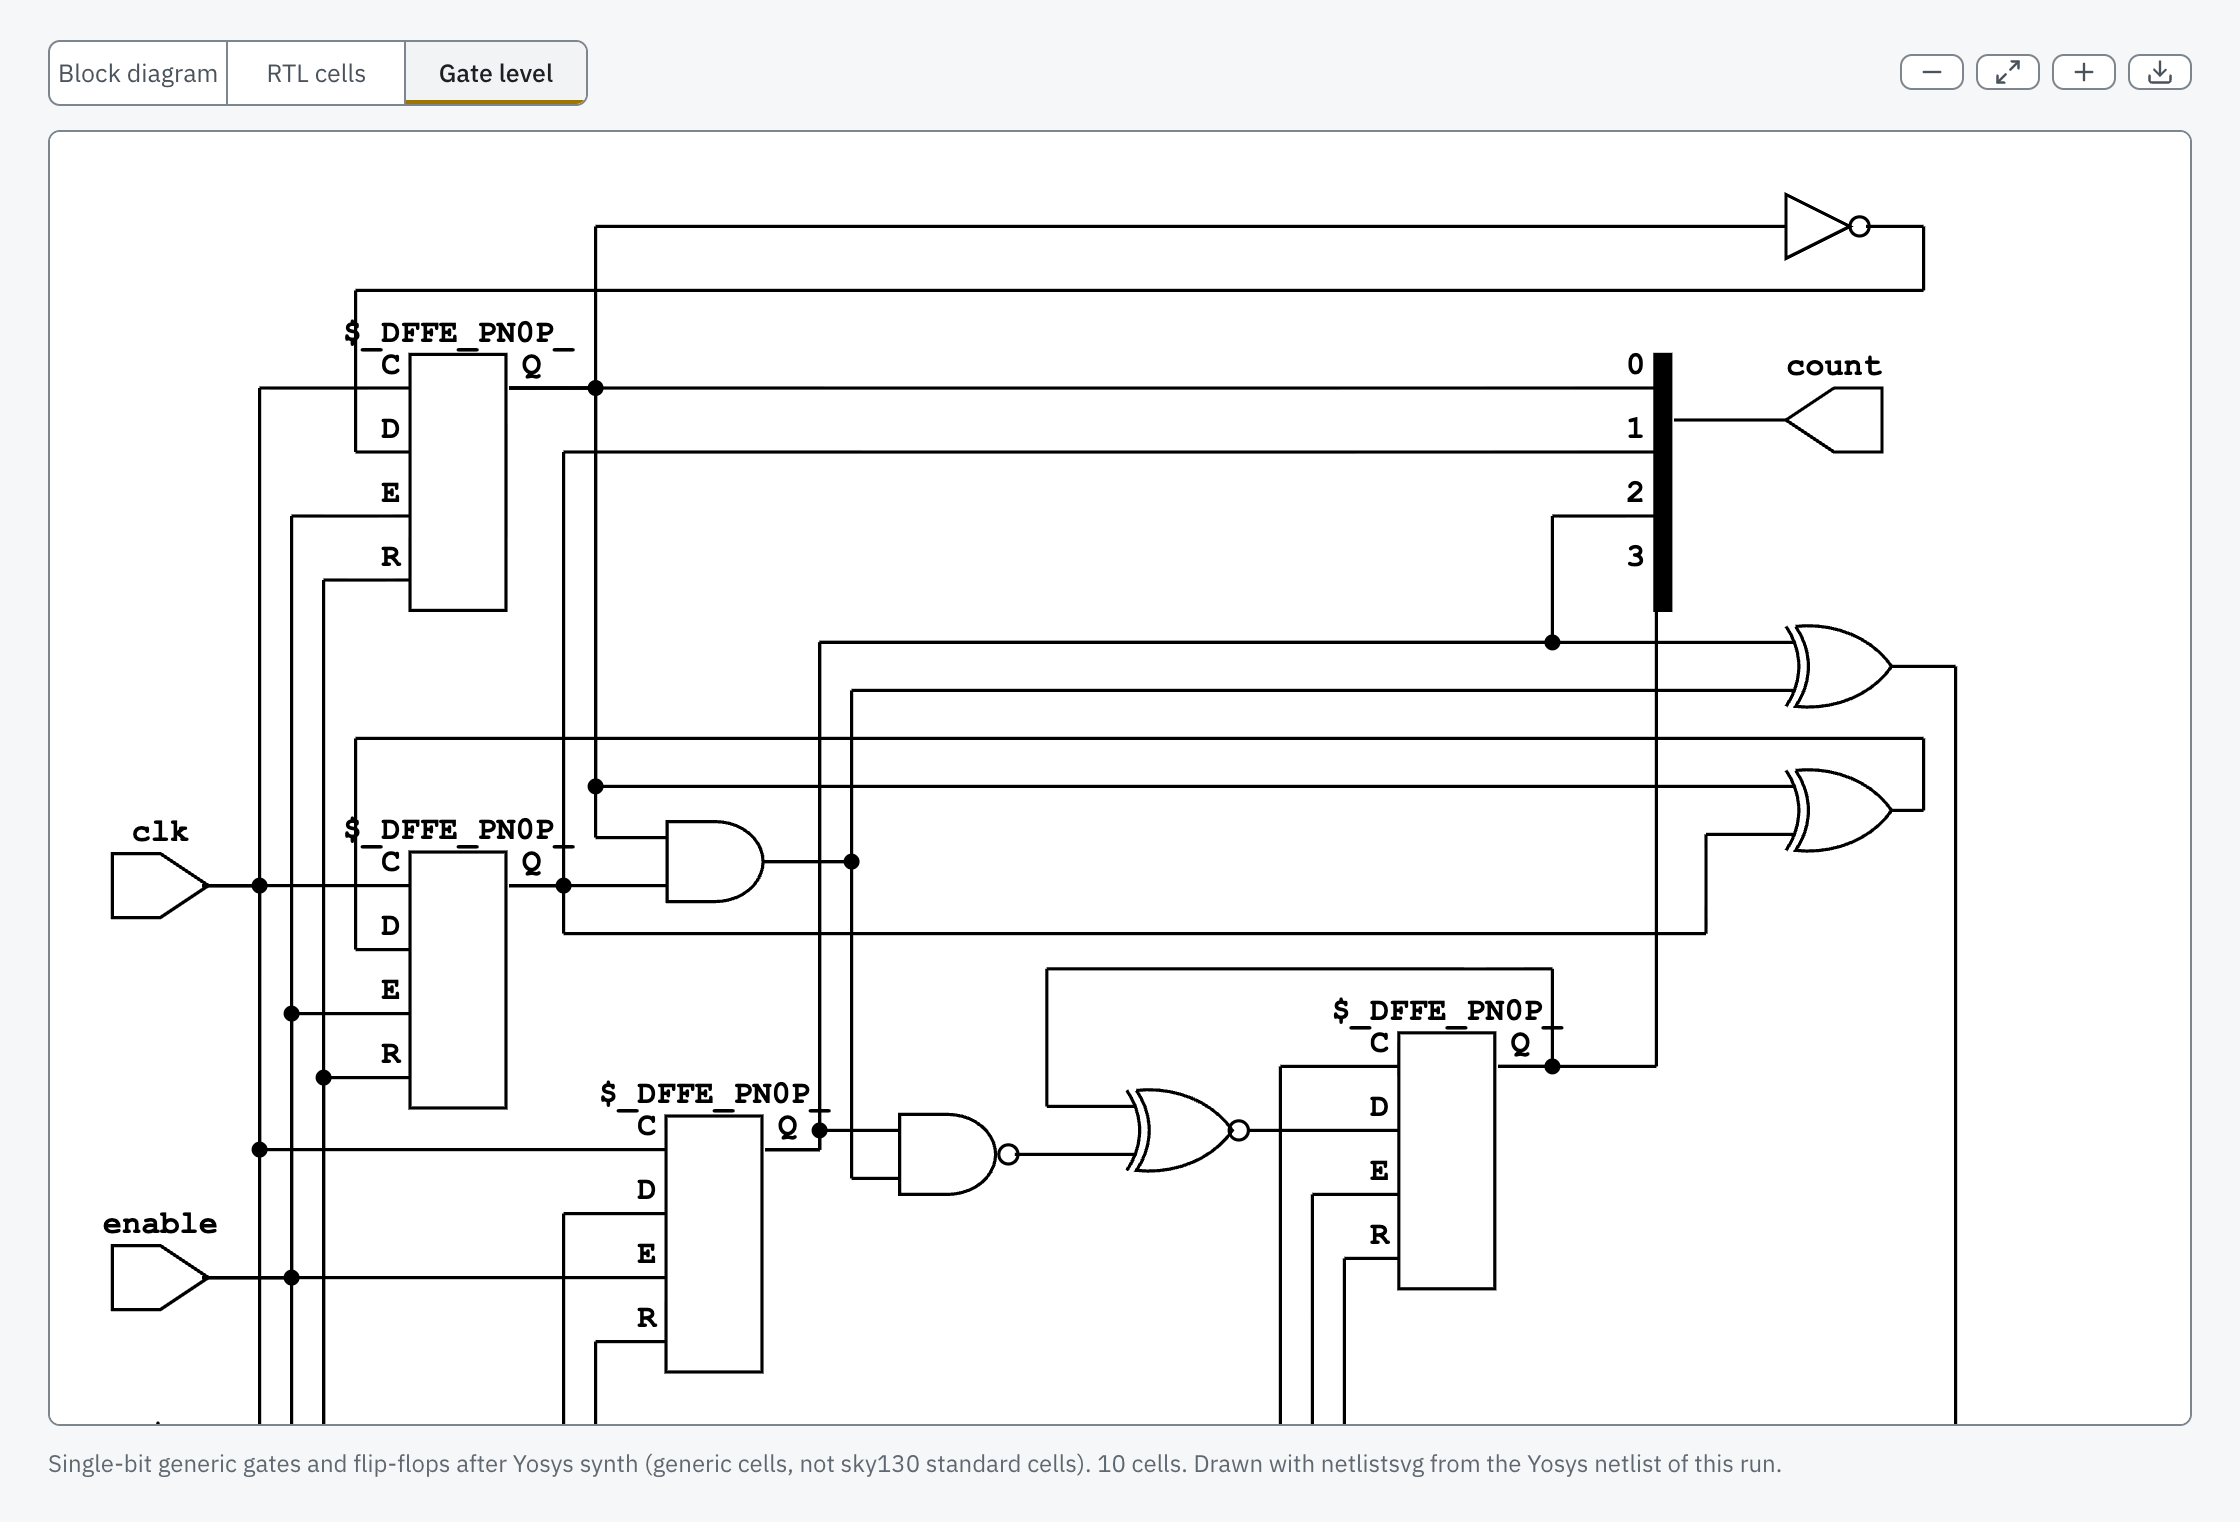
\includegraphics[width=0.7\textwidth]{s19_schematic_gate_level.png}
\caption[Gate level view of the schematic tab]{Schematic tab, ``Gate level'' view of the \emph{built-in} 4-bit counter (offline demo design): four enabled flip-flops with asynchronous reset and the XOR/NAND next-state logic. These are Yosys generic gates, not sky130 cells.}
\label{fig:schgate}
\end{figure}

\begin{figure}[htbp]
\centering
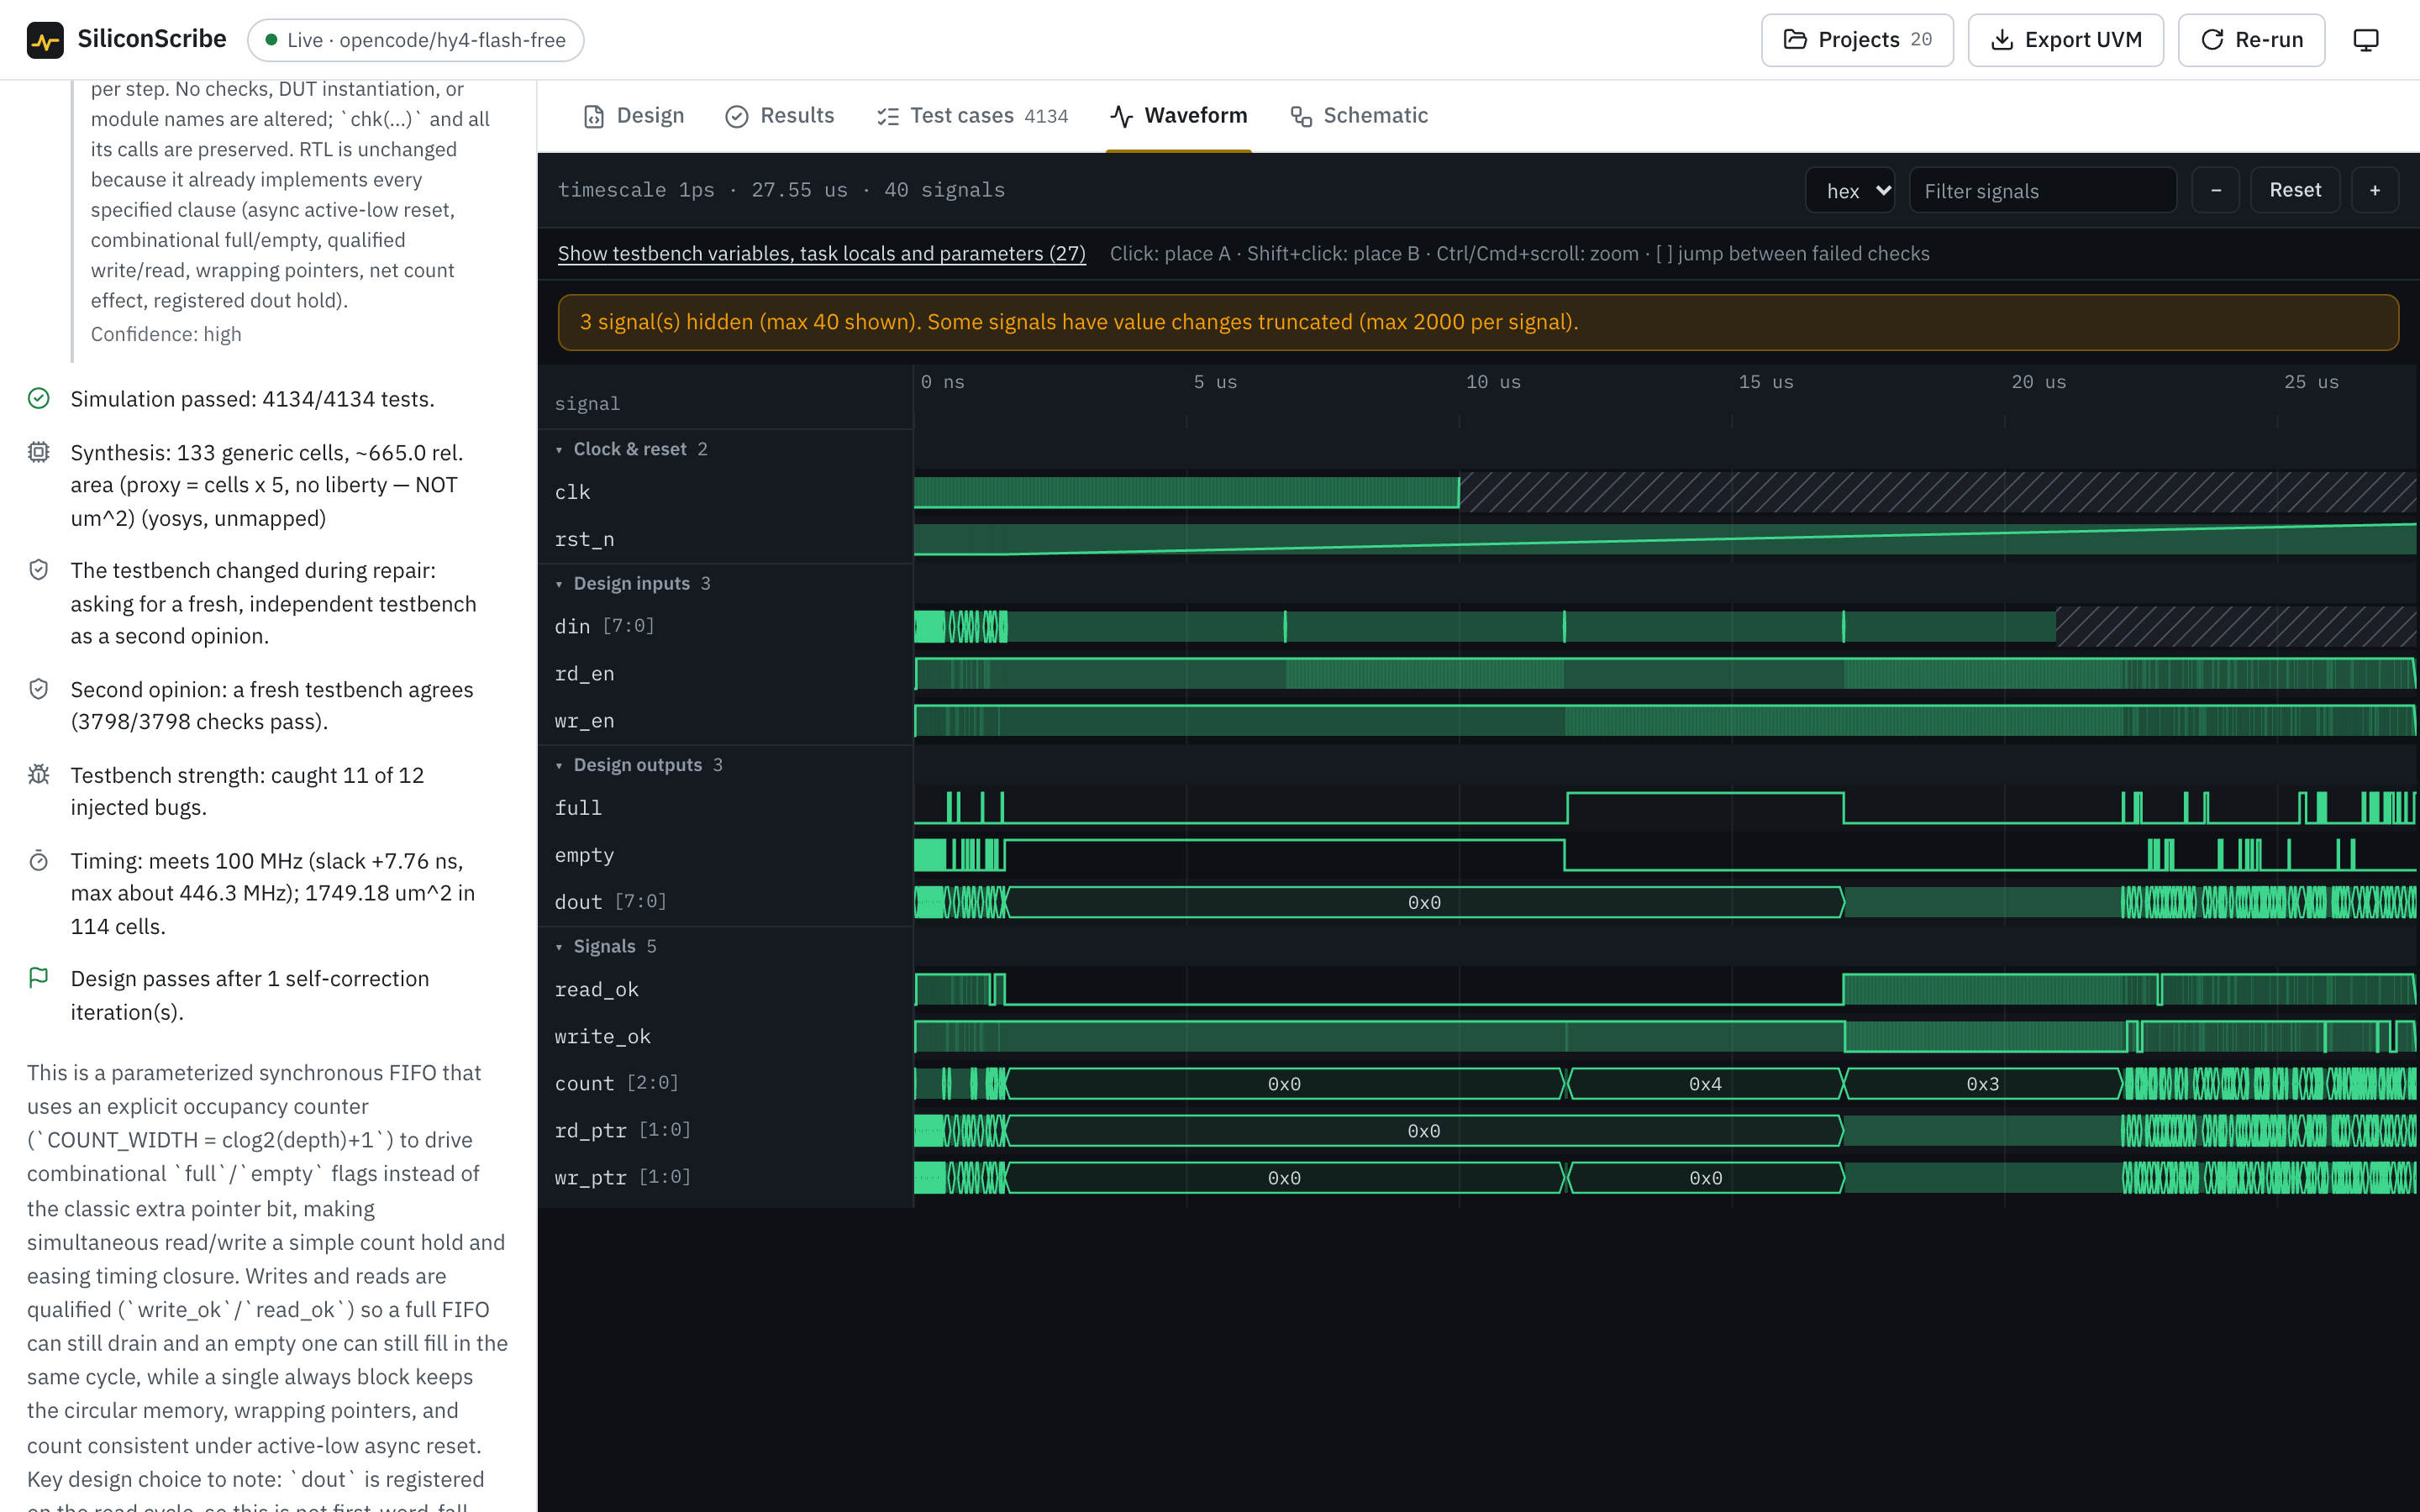
\includegraphics[width=0.7\textwidth]{s10_waveform.png}
\caption[Waveform tab of a live run]{Waveform tab of the live FIFO run, parsed from the simulator's VCD: signals grouped by role (clock and reset, design inputs, outputs, internal signals), hex radix, and a notice that some signals were hidden or truncated to keep the view bounded.}
\label{fig:cwave}
\end{figure}

\section{Project Persistence}
Finished runs are stored in SQLite and listed in the Projects menu with Load and Delete actions (Figure~\ref{fig:projects}). The first final review found that only the blocking route saved a project while the browser uses the streaming route, so nothing generated in the interface ever appeared in the list. The streaming route now persists the finished run, and a regression test pins it.

\begin{figure}[htbp]
\centering
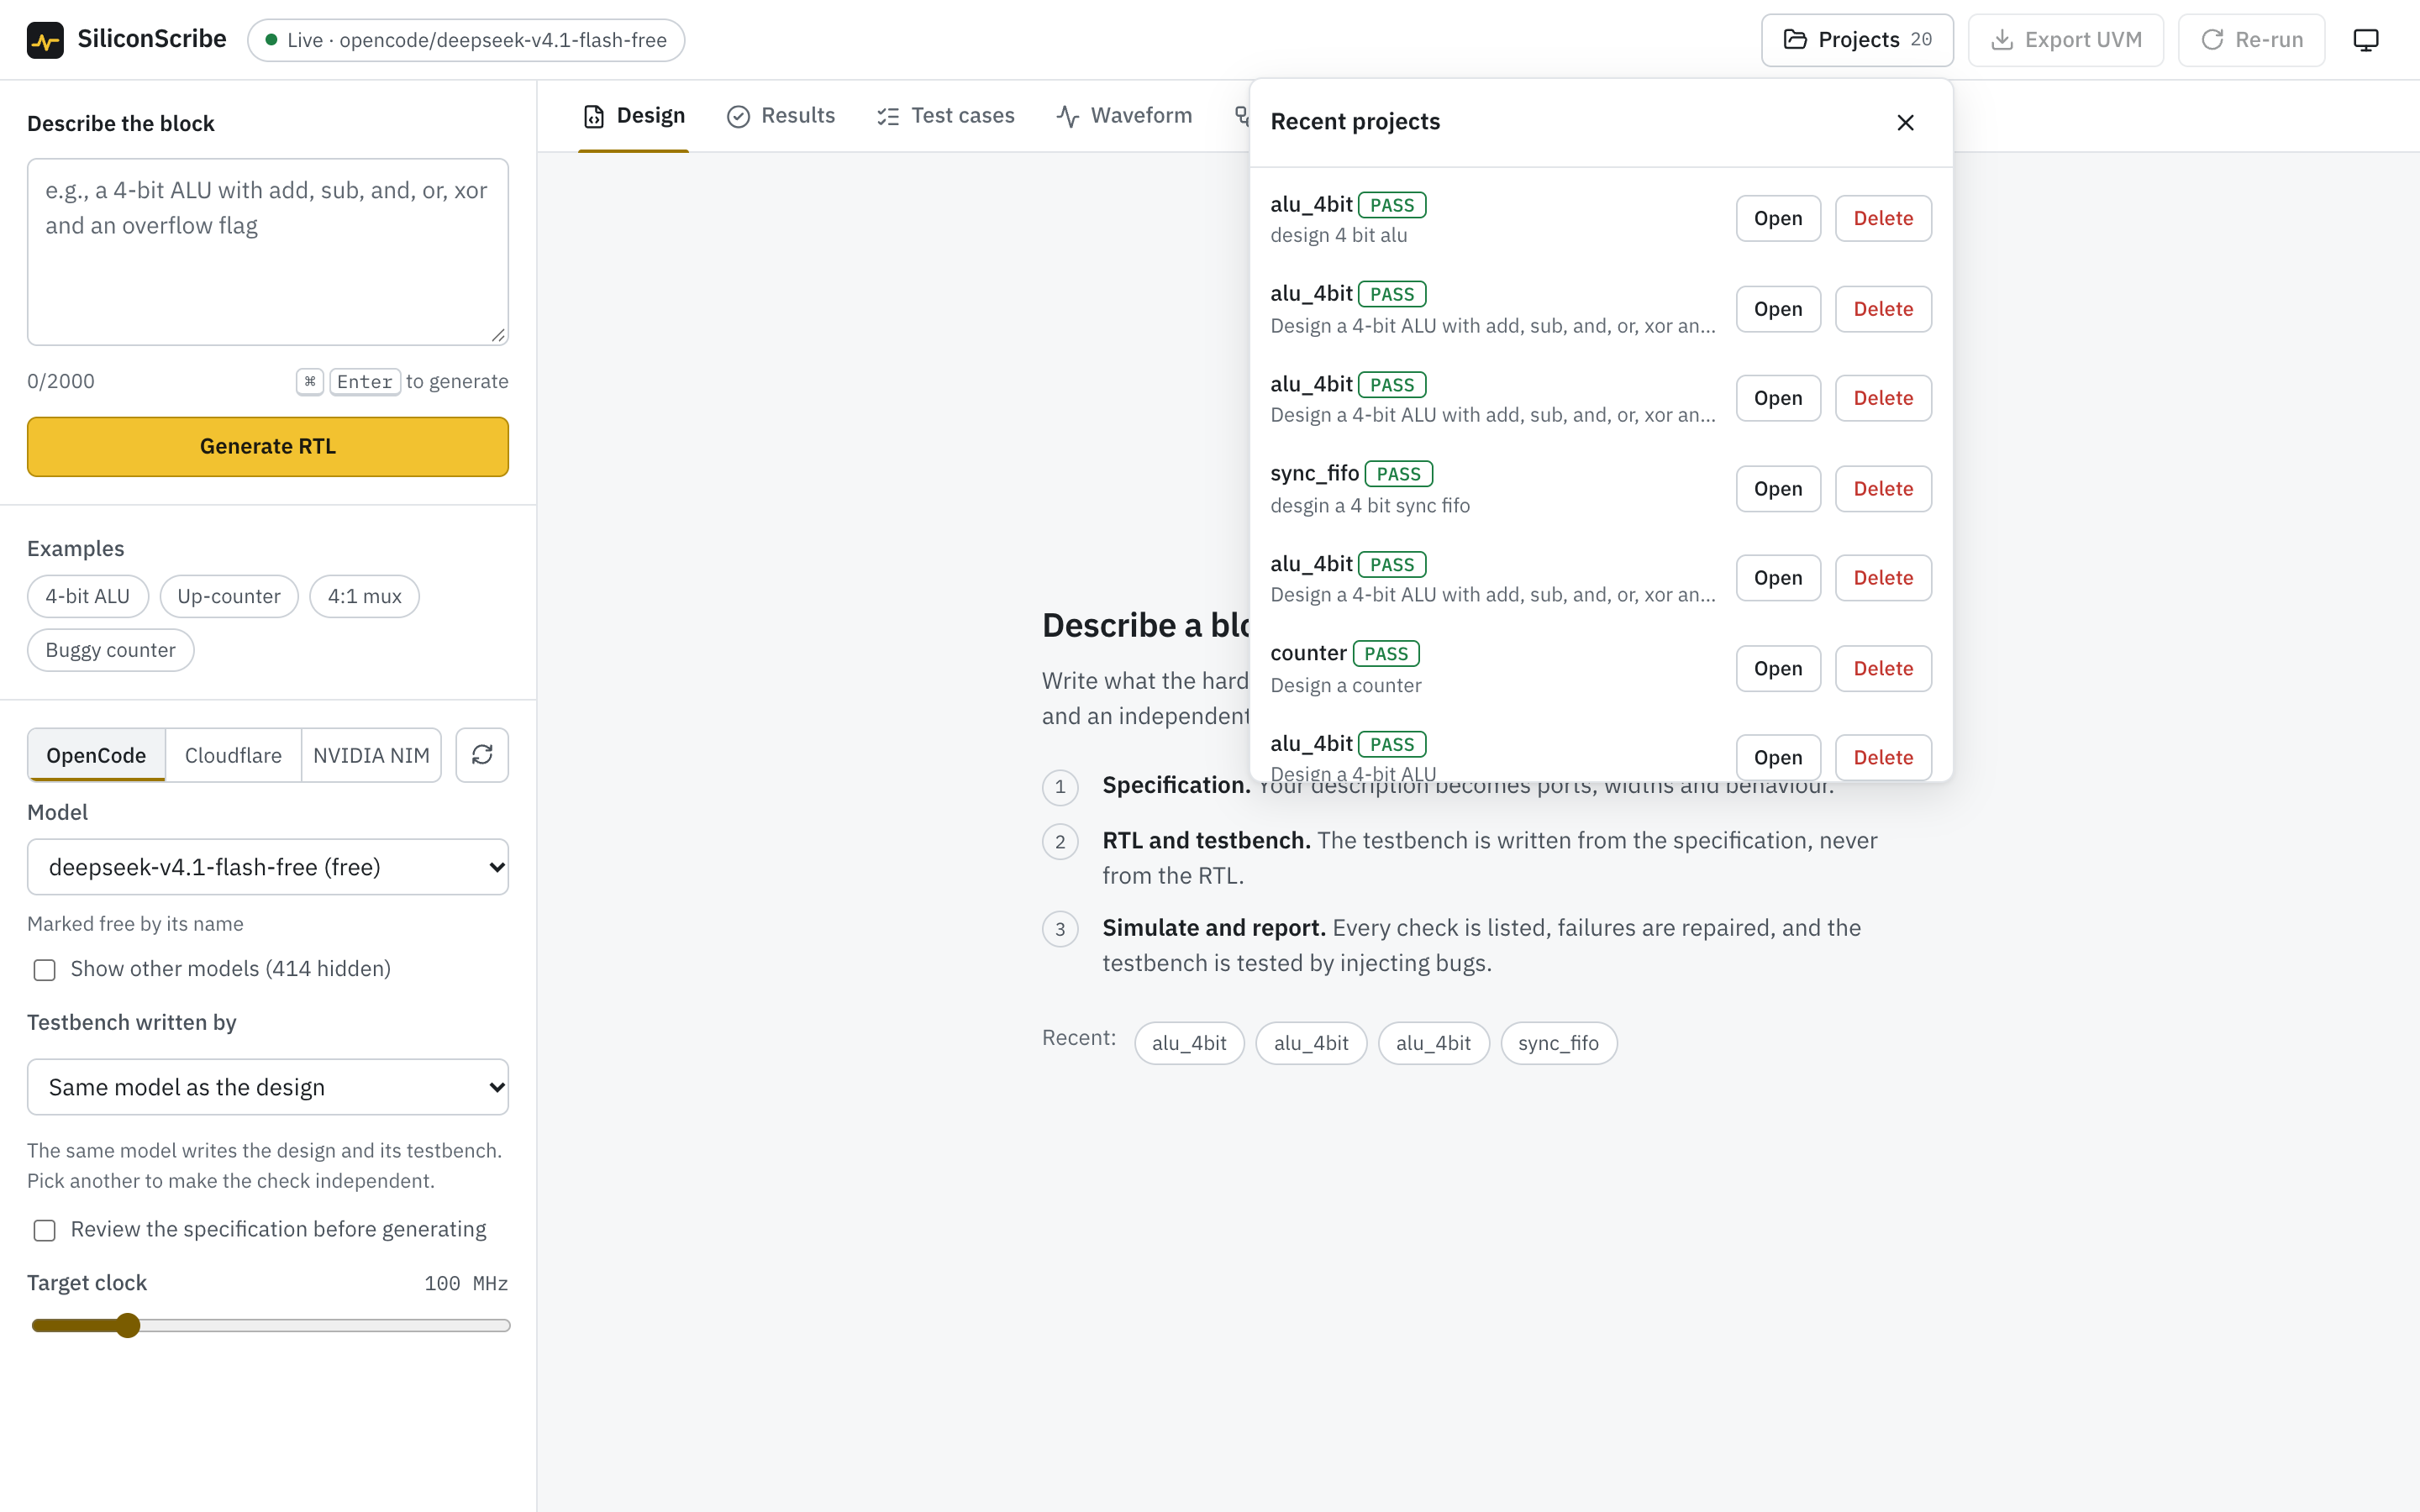
\includegraphics[width=0.5\textwidth]{s14_projects_menu.png}
\caption{The Projects menu listing saved runs.}
\label{fig:projects}
\end{figure}

\section{Degraded Mode in the Application}
When a prompt matches no curated design in offline mode, the interface shows a degraded-mode banner instead of passing a representative counter off as the requested design (Figure~\ref{fig:degraded}). In the capture a 16-bit barrel-shifter prompt, which no curated design implements, triggers it: the header says ``Demo fallback, not AI-generated'' and the results say that the built-in demo result was not generated by the AI model for the prompt. The strength, timing and toggle-coverage sections are still shown for the counter that actually ran.

\begin{figure}[htbp]
\centering
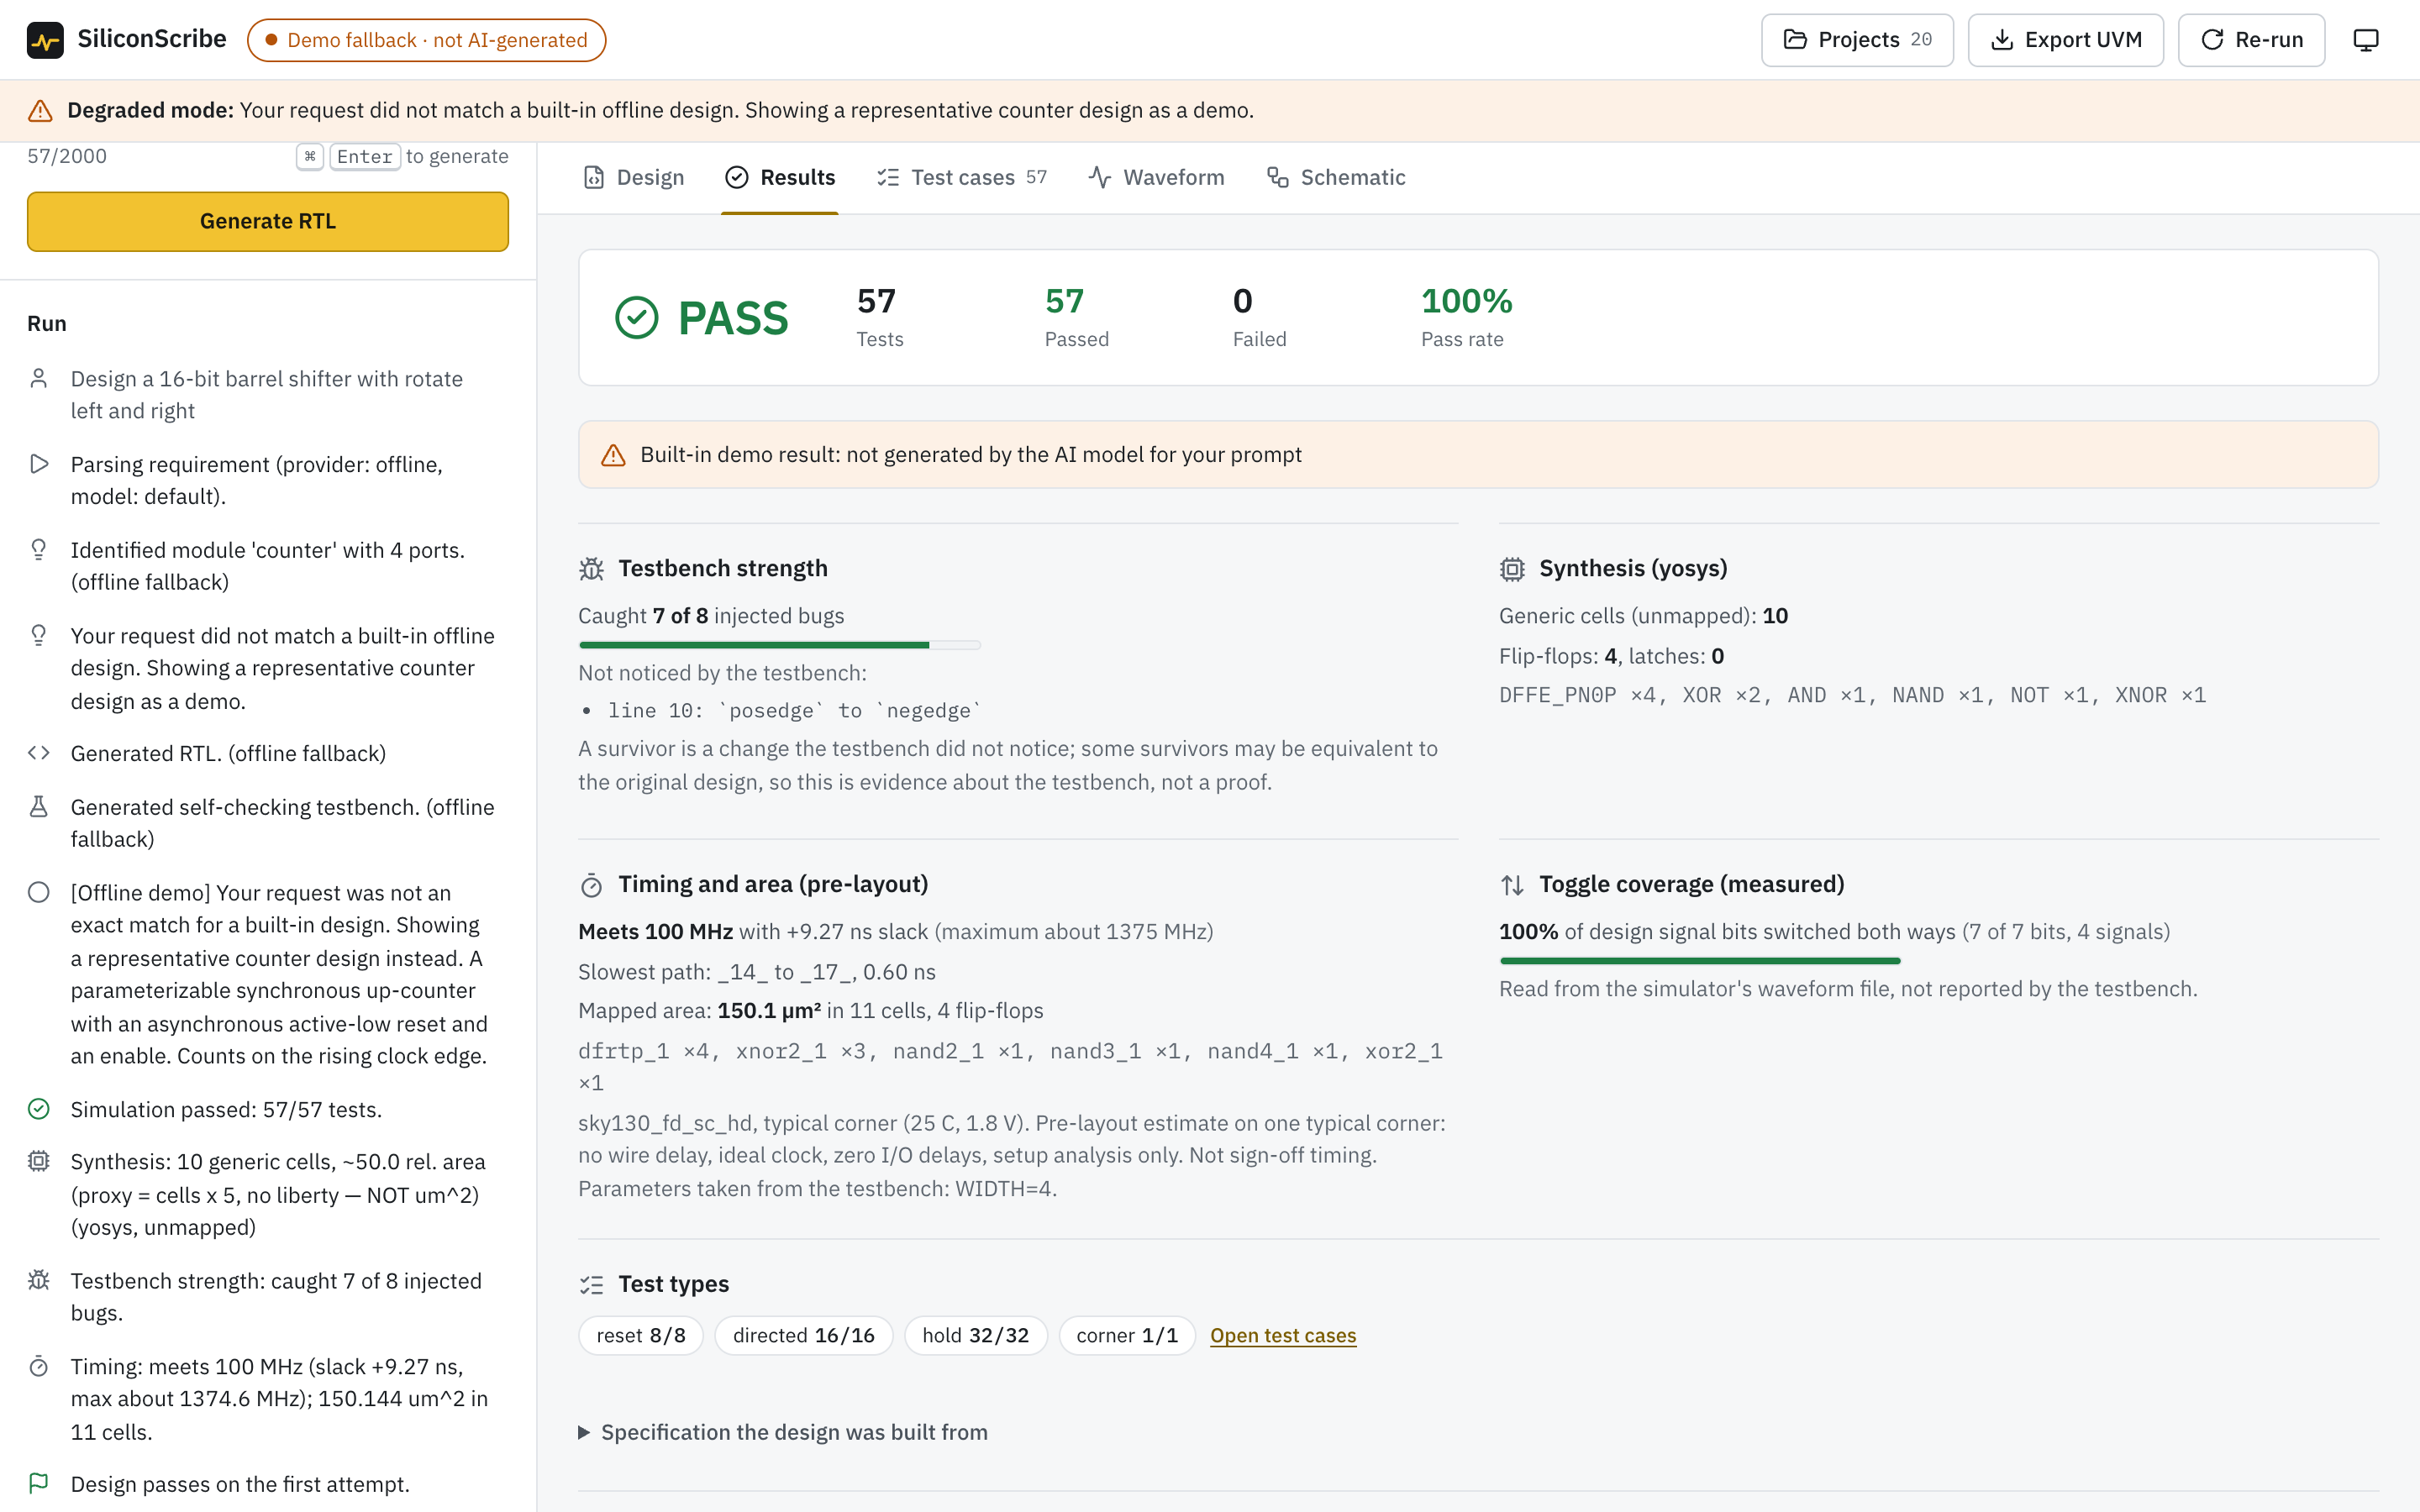
\includegraphics[width=0.65\textwidth]{s15_offline_demo.png}
\caption[Labelled fallback to the built-in demo]{A run that fell back to the built-in demo is labelled as such (degraded-mode banner and ``not generated by the AI model'' notice). The strength (7 of 8), timing (meets 100 MHz, 150.1\,\textmu m$^2$, 11 cells) and toggle-coverage sections describe the built-in counter that ran.}
\label{fig:degraded}
\end{figure}

\section{Final Security and Robustness Review}
\label{sec:review}
Before submission the system was probed the way an examiner or attacker might, using executable probes against the running API rather than code reading alone. Table~\ref{tab:review} lists the findings and their measured before/after behaviour. One suspected path was refuted: command execution through \code{$system()} does not work on Icarus Verilog 12.0, which reports the task as undefined; the sandbox policy still rejects it because other simulator builds define it.

\begin{table}[H]
\centering
\caption{Findings of the final review and their measured effect.}
\label{tab:review}
\footnotesize
\begin{tabularx}{\textwidth}{@{}p{3.1cm}p{3.7cm}p{3.2cm}X@{}}
\toprule
\textbf{Finding} & \textbf{Probe} & \textbf{Before} & \textbf{After} \\
\midrule
Testbench could read and write arbitrary files & planted secret file plus file-I/O tasks sent to the simulation endpoint & secret returned in the API response; file written outside the workspace & rejected by the sandbox policy; nothing leaked or written; 18 regression tests \\
One run froze the server & health check while an 8~s simulation runs & 6.5~s & 1~ms (blocking routes run in a thread pool; rate limiter locked) \\
Weak testbenches & 14-mutant sweep & 11 of 14 killed & 14 of 14 killed \\
Browser runs never saved & generate in the UI, open the drawer & not listed & listed; regression test \\
Tests wrote to the real database & row count before and after the suite & grew on every run & unchanged (isolated workspace) \\
Duplicated interface text & screenshots & bit range printed twice on waveform labels; degraded notice shown twice & each shown once \\
\bottomrule
\end{tabularx}
\end{table}

\subsection{Second review round}
\label{sec:review2}
After submission the whole system was reviewed again, this time by several independent reviewers (verification, security, backend design, interface and tests), and each claimed defect was reproduced before it was fixed. Table~\ref{tab:review2} lists what was found. Three results matter most for the question ``is a PASS trustworthy?'': the design under test could write its own verdict, the sandbox was a deny-list that could be sidestepped by task-name variants, and the repair loop could weaken the testbench that judges it.

\begin{table}[H]
\centering
\caption{Findings of the second review round (each reproduced, fixed and covered by a regression test).}
\label{tab:review2}
\footnotesize
\begin{tabularx}{\textwidth}{@{}p{3.2cm}p{4.0cm}p{3.0cm}X@{}}
\toprule
\textbf{Finding} & \textbf{Probe} & \textbf{Before} & \textbf{After} \\
\midrule
Forgeable verdict & wrong design whose own \code{initial} block prints \code{Passed: 200 / Failed: 0 / ALL TESTS PASSED}, optionally followed by \code{$finish} & reported PASS & design may not print the summary lines or end the run; summary must be whole lines, last pair wins; \code{FAIL}/\code{ERROR} lines contradict \code{Failed: 0}; zero checks is not a PASS \\
Sandbox deny-list gaps & file-access variants (\code{$fopena}, \code{$fputc}, \code{$ivlh_*}) & not on the deny-list & system tasks are allow-listed; anything else is rejected before compile \emph{and} before lint \\
Repair loop could weaken the oracle & fixer rewrites the testbench & accepted if it still printed PASS & minimum executed-check floor, design-instance check, original testbench re-run on the final design with an explicit warning if the oracle changed \\
Spoofable rate limit & 25 requests with a forged \code{X-Forwarded-For} & 25 of 25 accepted against 20 per minute & socket address used unless the deployment declares a trusted proxy \\
Resource limits & a testbench using about 1~GB for about 20~s & ran inside the old limits & CPU-time, file-size and memory limits plus at most two simulations at once (the memory limit is enforced on Linux, not macOS) \\
Re-run in the interface & edit the code and press Re-run & testbench checks skipped; previous waveform and warning left on screen & zero-check guard; waveform, repair timeline and warning refreshed; application-level regression test \\
Other correctness defects & a valid testbench with a one-second delay; port-width mismatches; multi-module replies; provider outages & false FAIL; hidden as warnings; truncated to the first module; recognised by digits in the message text & correct verdict; width mismatch is an error; all modules kept; typed upstream error \\
Weak curated testbenches & mutation sweep extended from 14 to 27 mutants & survivors found by the reviewers & 27 of 27 killed \\
Silently shortened test labels & a test type named \code{undefined_opcode} shown in the new Test cases tab & shown as \code{fined_opcode} (a Verilog string in a 12-character register keeps only its rightmost characters) & registers widened to 24 and 64 characters; a regression test runs a real simulation \\
\bottomrule
\end{tabularx}
\end{table}

The same review added a \emph{Test cases} tab to the results panel. It lists every executed check with its type (for example reset, directed, hold, exhaustive), its time, the expected and actual values and the result, with per-type pass ratios, filters, a bit-level difference for failures and a jump to that moment in the waveform. These rows are parsed from one \code{CHK|...} line per comparison; the verdict is decided by the validated summary, and since the fourth review round a \code{CHK|FAIL} row can only make it stricter (a FAIL), never turn it into a PASS. The waveform viewer was redesigned in the same round (signals grouped by role, value at the cursor, radix selection, two measurement cursors, flags at failed checks, fit-to-width zoom and a full-window mode).

\subsection{Third review round: timing stage and model access}
\label{sec:review3}
When the timing stage was added, it was attacked in the same way, by giving it designs chosen to break it. Table~\ref{tab:review3} lists what was found and fixed; its last two rows are defects of the later equivalence check, found when it was run on the evaluation designs, and each is now a regression test. The model menu was hardened at the same time: the API accepts browser calls from this machine only (extra exact origins are opt-in through \code{CORS_ALLOW_ORIGINS}), and every model id is validated before it can reach a subprocess or a URL (Section~\ref{sec:trustimpl}).

\begin{table}[H]
\centering
\caption{Defects found in the timing stage and its equivalence check, and their fixes.}
\label{tab:review3}
\footnotesize
\begin{tabularx}{\textwidth}{@{}p{4.0cm}p{4.6cm}X@{}}
\toprule
\textbf{Probe} & \textbf{Before} & \textbf{After} \\
\midrule
Design built from sub-modules & only the top module counted (area about 40\% too low); its clock was missed & hierarchy flattened before mapping \\
Clock not named \code{clk} & not recognised as a clock & clocks read from the mapped netlist; several clocks supported \\
Tri-state output & silently turned into a wire and reported as meeting 100 MHz & refused with a reason \\
Combinational loop & a meaningless maximum frequency & refused with a reason \\
Testbench overrides a parameter & a different circuit timed from the one simulated & numeric overrides applied before mapping \\
Equivalence check with \code{x} allowed on inputs & SAT ``disproved'' the correct ALU c7 with an input value containing \code{x} & inputs restricted to defined 0/1 values \\
Design built from an initialised array (c5) & equivalence check could not run (SAT cannot model memory initialisation) & RTL passed through Yosys \code{memory} first, as synthesis does \\
\bottomrule
\end{tabularx}
\end{table}

\subsection{Fourth review round: nine engineering roles}
\label{sec:review4}
Before the viva the whole tool (not the documents) was reviewed once more by nine reviewers, each taking one engineering role: ASIC design, design verification, backend systems, security, LLM integration, frontend, interface design, test engineering and release engineering. About 110 findings were reported; each was reproduced before it was fixed, every fix has a regression test, and each fix was checked by deliberately undoing it and confirming that a test fails. A tenth, independent reviewer then received only the findings and the change set, tried to break the fixes, and found a macro-argument sandbox bypass, a regular-expression slowdown introduced by the fixes and three regressions; those were fixed in the same way. All 123 saved runs and the 14 evaluation designs give the same verdicts with the old and the new code. Table~\ref{tab:review4} lists the findings that matter most.

\begin{table}[H]
\centering
\caption{Most important findings of the fourth review round (each reproduced, fixed and covered by a regression test).}
\label{tab:review4}
\footnotesize
\begin{tabularx}{\textwidth}{@{}p{4.2cm}p{4.4cm}X@{}}
\toprule
\textbf{Probe} & \textbf{Before} & \textbf{After} \\
\midrule
Testbench with a comment or a macro around \code{$dumpfile} / \code{$fopen} & wrote a file outside the workspace; run reported PASS & rules also applied after comment removal and to the macro-expanded source \\
Repair keeps the bug and edits the expected values & plain PASS, warnings only in text & shown as ``PASS, disputed''; the oracle may be rewritten only after a compile failure \\
Phase counters, \code{CHK|FAIL} rows, design forging the summary through \code{final} or \texttt{\%c} & PASS & FAIL, or refused before compiling \\
Port wider than 64 bits & upper bits never compared & check task widened to 256 bits; wider ports carry a warning \\
Slow one-check testbench in mutation testing & every timed-out mutant counted as caught (3 of 3) & timeouts of a slow testbench are inconclusive \\
64-bit register; slow path on a second clock & refused as ``no logic''; reported as meeting 500 MHz & timed correctly; misses timing \\
Flip-flop on the other clock edge; register with a declaration value & equivalence ``proven'' & ``not proven'' with the reason \\
Two runs of the same design at once & wrong verdict in 25 of 25 tries & one run per design folder at a time \\
Compile timeout & compiler child left at 100\% CPU & whole process group stopped; compile under CPU and memory limits \\
Quota error during a repair & whole run lost & run kept, with the reason \\
Partly unknown value shown in decimal & whole page blank & formatter never fails; error boundary around the results \\
Live run after the review: correct SR latch, testbench releases the forbidden input on both pins at once (zero-delay oscillation, simulated time stops) & TIMEOUT shown as ``0 checks, 0\%''; last output lost to \texttt{SIGKILL} & still TIMEOUT, but ``552 checks before stop'', no pass rate, and the likely cause named; \texttt{SIGTERM} first so the output is kept \\
\bottomrule
\end{tabularx}
\end{table}

\paragraph{What this does not establish.} The verdict is still only as strong as the testbench that prints it. Model-written testbenches are now measured on every PASS (strength, toggle coverage and, after a testbench-changing repair, a second opinion), but these measures are evidence, not proof: the strength score is a sample of up to 12 syntactic mutants and only toggle coverage is measured. The formal equivalence check covers only the step from RTL to netlist, not the RTL itself. The sandbox remains defence in depth on a developer machine, not a multi-tenant jail.

    \chapter{Discussion}
\label{ch:discussion}

This chapter interprets the results: the failure modes that shaped the design, how the system scales with stronger models, and how it was planned, deployed and costed.

\section{Engineering Findings}
\label{sec:discussion}

The final system is the product of several live failures. They are reported here
because they are the most transferable part of the work.

\begin{table}[H]
\centering
\caption{Live failure modes found during validation and their fixes.}
\label{tab:failures}
\footnotesize
\begin{tabularx}{\textwidth}{@{}p{3.9cm}p{5.3cm}X@{}}
\toprule
\textbf{Failure} & \textbf{Evidence} & \textbf{Fix} \\
\midrule
Reasoning tokens consumed the output budget & Empty \code{content}; the model's scratchpad was almost used as a testbench & Reasoning disabled by default; empty-content error is explicit; reasoning text is never returned as code \\
Silent mid-run offline swap & A live run failed at intent parsing and was replaced by a curated design & Disable fallback after the first successful live call; fail honestly \\
wire assigned in a procedural block & Icarus: ``not a valid l-value'' & Deterministic wire$\rightarrow$reg repair, scoped by file \\
\code{disable} inside a function & Icarus: ``cannot disable functions'' & Deterministic \code{disable}$\rightarrow$\code{return} repair \\
Testbench oracle width bug & 35-bit concatenation compared with a 4-bit output; expected and got printed identically & Prompt requires width-correct comparisons; fixer checks the oracle against the spec \\
Malformed JSON fix response & Unescaped Verilog quotes/newlines broke the parser & XML-section protocol plus tolerant JSON salvage \\
Model listing mismatch & UI offered a Zen model while OpenRouter was active; the run fell back & \code{/api/models} exposes only the configured model when it is not curated \\
TB-only fix discarded & The loop hashed only the RTL, so an oracle repair looked like a no-op & State hash covers RTL \emph{and} TB \\
Free model stalled on one prompt & s1 testbench generation timed out three times (Section~\ref{sec:eval}) & Per-run model menu; the run is reported as ``no result'', not as a failure \\
Watchdog shorter than the test & \code{gpt-oss-120b} testbench ended before printing its summary & ERROR with 0 checks; never PASS \\
Testbench sampled one cycle early & separate testbench model, FAIL 124/146 on a correct counter & failing checks not rewritten away; disagreement between the two models reported \\
\bottomrule
\end{tabularx}
\end{table}

Two conclusions follow. First, \textbf{the model is not the only source of bugs}:
the orchestrator, the prompt contract, the response parser, and the model catalog
all produced defects that looked like ``the LLM is weak.'' Second, \textbf{the
simulator is the right oracle}: every one of these defects was found by executing
the pipeline, not by reading the code.

Model choice also matters. The free Nemotron Lightning model produced plausible but
incorrect Boolean equations for the priority encoder; the larger
\code{nvidia/nemotron-3-ultra-550b-a55b:free} produced a correct \code{casez} chain
that passed the independent specification-derived testbench. The application therefore reports
the active model and does not pretend all models are equivalent.

\section{Scalability and Extensibility}
\label{sec:scale}

SiliconScribe was built model-agnostic and tool-agnostic. Every result in this report was obtained with free-tier language models because of budget, not because of an architectural limit. The model is chosen per run from the model menu (OpenCode, Cloudflare Workers AI, NVIDIA NIM), or any other OpenAI-compatible endpoint can be set through environment variables, so a stronger model is a configuration change, not a code change.

\subsection{Quality scales with the model}
The priority-encoder example of Section~\ref{sec:discussion} is a measured case: the same pipeline and simulator rejected one model's incorrect equations and passed a larger model's correct design on the first attempt. The evaluation gave a second case: the 4-bit counter prompt stalled three times on DeepSeek V4.1 Flash but passed on \code{opencode/hy4-flash-free} (Section~\ref{sec:eval}). A stronger model is expected to raise the first-attempt pass rate and reduce repairs, with the simulator still deciding PASS or FAIL.

\subsection{Per-stage model routing}
The pipeline already separates five model calls: specification parsing, RTL generation, testbench generation, explanation and diagnosis-and-repair. A deployment can route each to a different model with \code{LLM_MODEL_INTENT}, \code{LLM_MODEL_RTL}, \code{LLM_MODEL_TESTBENCH}, \code{LLM_MODEL_EXPLAIN} and \code{LLM_MODEL_FIX}. The sensible policy is to spend budget where correctness is decided, a strong model for the testbench and the diagnosis, and a cheap model for the cosmetic explanation. A model chosen explicitly per request still takes precedence, and the web interface's default selection does not disable routing. This is implemented and covered by automated tests. The interface also offers the most useful split directly: ``Testbench written by'' lets a different model, even from another provider, write the testbench (Section~\ref{sec:trustimpl}).

\subsection{Scaling dimensions}
\begin{table}[H]
\centering
\caption{What is in place today and the path to scale along each dimension.}
\label{tab:scale}
\footnotesize
\begin{tabularx}{\textwidth}{@{}p{2.5cm}XX@{}}
\toprule
\textbf{Dimension} & \textbf{In place today} & \textbf{Scaling path} \\
\midrule
Language models & Per-run model menu (OpenCode, Cloudflare Workers AI, NVIDIA NIM, read live); any OpenAI-compatible endpoint; per-request model and reasoning effort & Frontier and domain-tuned RTL models (for example VeriGen- or ChipNeMo-style) behind the same interface; automatic model selection driven by an evaluation suite \\
Stage routing & Five stage models by environment variable (implemented, tested) & Cost, latency and accuracy aware routing policy; fallback chains \\
Verification strength & Specification-only testbench; anti-cheat guard; mutation score and toggle coverage on every PASS; optional separate testbench model; second opinion; specification review & Golden reference models; SVA assertions and formal equivalence; line and branch coverage; coverage-directed stimulus \\
Machine-learning models beyond LLMs & Clear seams: spec parsing, stimulus, diagnosis & Learned stimulus and coverage-closure agents; retrieval of similar verified designs as examples; learned bug localisers that rank suspicious RTL lines from failing vectors \\
EDA toolchain & Icarus Verilog; Yosys and OpenSTA on the sky130 library for a pre-layout timing and area estimate; Verilator lint hook; OpenROAD stub & Place and route with OpenROAD for post-layout timing; more corners; line and branch coverage with a simulator that supports the generated testbenches \\
Runtime & Single FastAPI process; blocking routes in a thread pool; SQLite; in-memory rate limiter & Job queue and worker pool; container or microVM sandbox per simulation; PostgreSQL; authentication and tenancy; object storage; metrics and tracing \\
Design size & Single blocks; evaluated on blocks under about 100 lines & Hierarchical decomposition: specification to sub-blocks to integration tests \\
\bottomrule
\end{tabularx}
\end{table}

\subsection{What this does and does not claim}
Model quality is shown above to matter, and the routing seam is implemented. Scaling to many concurrent users needs the runtime items in Table~\ref{tab:scale} (the deployment today is a single node with an in-process rate limiter and a local database); these are additions around an unchanged core, not a redesign.

\section{Project Timeline, Deployment and Cost}
\label{sec:project}

\subsection{Development timeline}
\begin{table}[H]
\centering
\caption{Milestones (from the repository history and dated artefacts).}
\label{tab:timeline}
\footnotesize
\begin{tabularx}{\textwidth}{@{}p{2.6cm}X@{}}
\toprule
\textbf{Date (2026)} & \textbf{Milestone} \\
\midrule
23 July & Baseline; Docker, CI/CD, structured logging, health check, rate limiting, no-progress guard, VCD truncation metadata, frontend and backend tests \\
29 August & Zero-budget provider, hardening, lint and synthesis wrappers, SQLite projects, UVM export; QA and security audit \\
4--5 September & Vercel and Render free-tier deployment, live provider, 8-bit ALU, real reasoning-effort levels, CORS and rate-limit fixes \\
15 October & Progress report \\
September--November & Specification-only testbenches, structured diagnosis, compiler repairs, honest degraded mode, live validation \\
6 November & Live evidence captured; final review (sandbox, server freeze, testbench hardening, persistence fix, model routing); final report and presentation \\
November (after 6 Nov.) & Second review round; testbench strength by mutation, measured toggle coverage, Yosys and OpenSTA timing and area on sky130, model menu (OpenCode, Cloudflare, NVIDIA NIM), specification review, separate testbench model, second opinion, CORS hardening, live evaluation on fifteen prompts \\
19 November & Final verification of the tool (Table~\ref{tab:verify}) \\
\bottomrule
\end{tabularx}
\end{table}

\subsection{Deployment}
A multi-stage Docker image builds the frontend with Node 20 and serves it from a Python 3.12 image that also contains Icarus Verilog and Yosys, with a health check on \code{/health}. The configuration targets Vercel for the static frontend (which rewrites \code{/api} to the backend) and Render for the backend container; free tiers sleep when idle, so the interface explains cold-start delays. Docker Compose runs the whole system locally in one container. The image does not yet include OpenSTA or the sky130 library, so inside the container the timing and area estimate reports itself as not available.

\subsection{Cost}
Development and validation cost nothing beyond the laptop: open-source tools and free-tier models (free OpenCode models, the Cloudflare Workers AI free allowance of 10,000 neurons a day, and the NVIDIA NIM free queue). The price of free models is time and quota: a live run took a median of 360~s. When scaling, cost is driven by tokens per model call times calls per run, plus hosting. Per-stage routing keeps the expensive model on the testbench and diagnosis stages only, and the deterministic compiler repairs avoid model calls altogether for mechanical errors.

\subsection{Third-party components}
Icarus Verilog (GPL-2.0), Yosys (ISC), OpenSTA (GPL-3.0), the SkyWater SKY130 library (Apache-2.0), FastAPI and Pydantic (MIT), Uvicorn (BSD-3-Clause), React, Vite and CodeMirror (MIT) and SQLite (public domain). Generated designs belong to the user; no user data leaves the server except the prompt and code sent to the chosen model provider (or two providers when a separate testbench model is chosen).

    \chapter{Conclusion and Future Work}
\label{sec:conclusion}

\section{Conclusion}
SiliconScribe works as an execution-grounded RTL assistant rather than a scripted
demonstration. A plain-English prompt is parsed into a specification, which the user
can review and edit; RTL and an independent, specification-derived testbench are
generated; Icarus Verilog executes them; and failures produce a structured,
line-level diagnosis that is patched and re-simulated. The simulator decides PASS or
FAIL, never the model. Around that loop the system measures how much a PASS is worth:
testbench strength by mutation testing, measured toggle coverage, a second-opinion
testbench after a testbench-changing repair, an optional separate model for the
testbench, and a pre-layout timing and area estimate on the SkyWater 130\,nm library.

In a live evaluation with one free model, 14 of 15 prompts completed: 8 passed on the
first attempt and 6 after one self-repair, and hand-written reference testbenches
confirmed that all 14 final designs are correct. The fifteenth prompt timed out three
times and is reported as no result. The tool itself is checked by 436 backend and 211
frontend tests, a 27-of-27 mutation sweep, a gate-level equivalence check of the
timing stage on 19 designs, and an accessibility audit with no violations.

Because the pipeline is model-agnostic, its quality is expected to rise with better models (a larger model already turned an incorrect priority encoder into a first-attempt PASS), and the remaining work is mostly infrastructure and stronger verification rather than redesign (Section~\ref{sec:scale}).

The most important engineering lesson is that \emph{honesty is a feature}. The
system labels compiler repairs, refuses to delete checks, refuses to swap designs
mid-run, refuses to time circuits it cannot time honestly, reports a stalled model as
``no result'', reports when two models disagree, and distinguishes a scripted offline
fix from a live diagnosis. Those choices make the PASS meaningful. A PASS is still
evidence, not proof.

\section{Limitations}
\label{sec:limits}

\begin{enumerate}[label=\textbf{L\arabic*.},ref=L\arabic*]
\item \textbf{Residual common-mode model risk.} The testbench never sees the RTL,
but unless a separate testbench model is chosen, the same model interprets the
specification for both. If it misreads the specification identically in both, the
pair can still agree while being wrong. The specification is also written by a model
unless the user reviews it. The separate testbench model, the specification review
and the second opinion reduce this risk; they do not remove it, and the application
does not decide automatically which side of a disagreement is wrong.
\item \textbf{Strength is a sample.} The strength score uses up to 12 syntactic
one-token mutants. A survivor may be an equivalent mutant, and a high score does not
prove the testbench complete.
\item \textbf{Only toggle coverage is measured.} Line and branch coverage are not
measured; Verilator could not build most of the generated testbenches. Any other
coverage figure is what the testbench reports about itself and is labelled as such.
\item \textbf{No assertions or formal checks.} There are no SVA properties and no
formal equivalence check; the only oracle is the simulated testbench.
\item \textbf{Timing is a pre-layout estimate.} One typical corner, no placement or
routing (no wire delay), an ideal clock, zero I/O delays and setup analysis only.
Power is not reported. Designs with tri-states, latches, loops or derived clocks are
refused rather than timed. It is not sign-off.
\item \textbf{Small evaluation.} The evaluation used small blocks (under about 100
lines), one run per prompt and mainly one model, so it does not support pass-rate
comparisons with published benchmarks.
\item \textbf{Free models are slow and quota-limited.} A live run took a median of
360~s, some free-queue models took minutes per reply, Cloudflare's free allowance is
10,000 neurons a day, and models are retired without notice. GitHub Copilot through
OpenCode is available only as \code{github-copilot/auto}, which cannot name the model
it used.
\item \textbf{UVM export is not compiled.} The 16-file UVM 1.2 bundle targets a
commercial simulator; Icarus cannot compile UVM and no commercial licence was
available. It is a structural export, not a verified UVM testbench.
\item \textbf{Not a hardened sandbox.} Generated Verilog runs as a local \code{vvp} subprocess with the server's privileges. The sandbox policy (Section~\ref{sec:sandbox}), the scrubbed environment, the resource limits and the output cap reduce the attack surface (the memory limit is enforced on Linux only), but a static scan of Verilog cannot be airtight; multi-user deployment requires a container or microVM per simulation.
\item \textbf{Single-node runtime.} The rate limiter is in-process, persistence is a local SQLite file and simulations share one host; concurrency is bounded by the thread pool rather than by a queue (Section~\ref{sec:scale}).
\end{enumerate}

\section{Future Work}
\begin{enumerate}[label=\textbf{\arabic*.}]
\item \textbf{Multi-model comparison} on the fifteen evaluation prompts, with the
reference check and the strength score reported per model.
\item \textbf{Assertions and formal checks:} SVA properties as a second oracle
alongside the self-checking testbench, and formal equivalence where a reference
exists.
\item \textbf{Line and branch coverage} with a simulator that supports the generated
testbenches.
\item \textbf{Place and route with OpenROAD} for post-layout timing with real wire
delay.
\item \textbf{Gate-level visualisation} of the mapped netlist in the schematic tab.
\item \textbf{Production runtime:} container isolation per simulation and a job queue
for multi-user use, with PostgreSQL and authentication (Section~\ref{sec:scale}).
\item \textbf{Code structure:} split the pipeline function (about 500 lines) into
smaller stages that can be tested on their own.
\end{enumerate}


    % -------------------------------------------------------------------
    % Bibliography
    % -------------------------------------------------------------------
    \nocite{*}
    \bibliography{references}

    % -------------------------------------------------------------------
    % Appendices
    % -------------------------------------------------------------------
    \begin{appendices}
        \chapter{Reproduction}
\label{app:repro}

\section{Running the system}
\begin{lstlisting}[language=bash,basicstyle=\ttfamily\scriptsize]
# Tools: Icarus Verilog 12.0; for timing and area also Yosys, OpenSTA (sta)
# and the sky130 liberty file (see backend/pdk/README.md)
cd backend
export PATH="$HOME/.local/bin:$PATH"

# Offline demo (built-in designs, no model calls)
OFFLINE_MODE=1 python3 main.py

# Live backend through the OpenCode app; model keys for Cloudflare
# Workers AI and NVIDIA NIM are read only from backend/.env
env -u OFFLINE_MODE LLM_PROVIDER=opencode-app \
  LLM_MODEL=deepseek-v4.1-flash-free python3 main.py

# Any other OpenAI-compatible endpoint (example: OpenRouter)
env -u LLM_PROVIDER -u OPENCODE_API_KEY -u ZEN_API_KEY -u NVIDIA_API_KEY \
  OPENAI_API_KEY=... OPENAI_BASE_URL=https://openrouter.ai/api/v1 \
  LLM_MODEL=nvidia/nemotron-3-ultra-550b-a55b:free python3 main.py

# Frontend dev server
cd ../frontend && npm run dev -- --host 127.0.0.1
\end{lstlisting}

\section{Verifying the tool}
\label{app:verify}
These commands reproduce Table~\ref{tab:verify}. All except the last make no model
calls.
\begin{lstlisting}[language=bash,basicstyle=\ttfamily\scriptsize]
cd backend
export PATH="$HOME/.local/bin:$PATH"
OFFLINE_MODE=1 python3 -m pytest            # 453 passed
python3 tools/mutation_sweep.py             # 27/27 injected bugs caught
python3 tools/verify_mapping.py             # 19/19 designs, same results at gate level
python3 evaluation/independent/run.py       # 14/14 evaluated designs correct
python3 evaluation/independent/strength.py  # strength of the reference testbenches
python3 tools/preflight.py --live           # one small model call; fallback ladder

cd ../frontend
npx tsc -b && npx vitest run && npm run build   # 222 passed
\end{lstlisting}

The live evaluation of Section~\ref{sec:eval} is re-run with
\code{python3 tools/evaluate_live.py} (it resumes and skips prompts that already
have a record); \code{--summary} only rebuilds \code{evaluation/summary.md} from the
saved records in \code{evaluation/results.jsonl}.

The live harness used for the earlier priority-encoder and seeded-bug runs calls
the same event generator as the web API (\code{pipeline_events}). The resulting RTL,
testbench, simulator transcript, and structured diagnosis are archived under
the directory \path{docs/evidence/} for audit.


\chapter{Complete Prompt Set}
\label{app:prompts}
The system prompts below are extracted from \code{backend/llm_service.py} (only the dashes are changed for typesetting). The same testbench prompt is used for a separate testbench model and for the second-opinion testbench.
\lstset{basicstyle=\ttfamily\tiny,language=,breaklines=true,frame=single}
\section{Specification parser}
\lstinputlisting{appendix/prompt_intent.txt}
\section{RTL generator}
\lstinputlisting{appendix/prompt_rtl.txt}
\section{Independent testbench generator}
\lstinputlisting{appendix/prompt_testbench.txt}
\section{Debugger (diagnosis and repair)}
\lstinputlisting{appendix/prompt_fix.txt}

\chapter{Live-Generated Testbench}
\label{app:tb}
The specification-derived testbench generated live for the priority encoder of Chapter~\ref{sec:results} (archived as \code{docs/evidence/livepriority08_testbench.sv}), followed by the simulator transcript.
\lstinputlisting[style=vlog,basicstyle=\ttfamily\tiny]{evidence/livepriority08_testbench.sv}
\lstinputlisting[language=,basicstyle=\ttfamily\tiny]{evidence/livepriority08_transcript.log}

    \end{appendices}

\end{document}
